\documentclass{report}
\usepackage[utf8]{inputenc}
\usepackage{amsmath,amsthm,amssymb,graphicx,setspace,mathrsfs,mathstyle,listings,color}
\usepackage{csvsimple,longtable}
%\topmargin 0in
%\headheight 0in
%\headsep .2in
%\textheight 220mm
%\textwidth 159mm
%\oddsidemargin 0in
%\evensidemargin 0in

\newtheorem{theorem}{Theorem}[section]
\newtheorem{lemma}[theorem]{Lemma}
\newtheorem{proposition}[theorem]{Proposition}
\newtheorem{conjecture}[theorem]{Conjecture}
\newtheorem{question}[theorem]{Question}
\newtheorem{corollary}{Corollary}[theorem]

%\theoremstyle{definition}
\newtheorem{definition}[theorem]{Definition}
\newtheorem{example}{Example}

\theoremstyle{remark}
\newtheorem{remark}{Remark}

\numberwithin{equation}{section}

\definecolor{codegreen}{rgb}{0,0.6,0}
\definecolor{codegray}{rgb}{0.5,0.5,0.5}
\definecolor{codepurple}{rgb}{0.58,0,0.82}
\definecolor{backcolour}{rgb}{0.95,0.95,0.92}
 
\lstdefinestyle{mystyle}{
    backgroundcolor=\color{backcolour},   
    commentstyle=\color{codegreen},
    keywordstyle=\color{magenta},
    numberstyle=\tiny\color{codegray},
    stringstyle=\color{codepurple},
    basicstyle=\footnotesize,
    breakatwhitespace=false,         
    breaklines=true,                 
    captionpos=b,                    
    keepspaces=true,                 
    numbers=left,                    
    numbersep=5pt,                  
    showspaces=false,                
    showstringspaces=false,
    showtabs=false,                  
    tabsize=2
}

\lstset{style=mystyle}

\title{The Ulam sequence and related phenomena}
\author{Daniel Ross}
\date{ }

\begin{document}
\maketitle

\tableofcontents

%%%%%%STARTDOC

\chapter{Introduction}

The Ulam sequence, defined by Stanislaw Ulam in \cite{ulam:siam1964},
is a sequence $a_n$ of positive integers that is given by the folowing
recursive definition: It starts with $a_1 = 1$, $a_2 = 2$, and then
for $n > 2$, $a_n$ is the integer satisfying:
\begin{enumerate}
\item It is expressible as a sum of distinct previous Ulam numbers in
  exactly one way: There is exactly one pair of $0 < i < j < n$ with
  $a_i + a_j = a_n$.
\item It is larger than the previous element of the sequence: $a_n >
  a_{n-1}$.
\item It is the smallest positive integer with the above two
  properties.
\end{enumerate}

Thus the first few terms can be computed: 

\[1, 2, 3, 4, 6, 8, 11, 13, 16, 18, 26, 28, 36, 38, 47, 48, 53, 57, 62,
69, \ldots\]

In particular, there are two ways a number could fail to be Ulam:
Either it has a representation as a sum of two distinct smaller Ulam
numbers in more than one way (such as $5 = 4+1 = 2+3$), or it has no
representations as a sum of distinct smaller Ulam numbers at all (such
as 23).

One thing that makes the sequence interesting is that it seems
historically to have been very difficult to prove anything about it.
We know, for example, that it must be infinite: given the first $n$
elements $a_1, \ldots, a_n$, we can always find at least one number
that satisfies the first two criteria above, namely
$a_{n-1} + a_{n-2}$.  Thus there must be a smallest such number, which
is therefore the next Ulam number.  However we do not know whether
this sequence has positive density in any sense.

We also know that if we use the same definition but start with
different initial values, we can get sequences that we can analyse
very easily indeed: If the ``$(u,v)$-Ulam sequence'', denoted
$\ulam{u}{v}$, is the sequence with $a_1 = u, a_2 = v$, and $a_n$ (for
$n > 3$) defined exactly as before, then by a theorem of Schmerl and
Speigel \cite{schmerl:jct1994} we know that the $(2,v)$-Ulam sequence,
in the case where $v$ is odd and at least 5, is regular in the
following sense:

\begin{definition}\label{def:regularity}
  An increasing, infinite sequence $\{a_i\}$ of positive integers is
  \textbf{regular} if the sequence $\{b_i = a_i - a_{i-1} : i > 1\}$
  is eventually periodic.
\end{definition}

Regular sequences are very easy to describe--we could specify them
(after some initial segment) by a set of congruence classes modulo
some (possibly large) $m$.  In particular, a regular sequence
$\ulam{u}{v}$ will be far easier to compute than the definition would
naively suggest.

There are other initial values that are variously known to or believed
to give rise to regular sequences, also.  See, for example,
\cite{finch:em1992}.  That said, many Ulam-type sequences appear not
to be regular, among them $\ulam{1}{2}$ and $\ulam{2}{3}$.  So we
might wonder if these exhibit some other kind of similar pattern,
though perhaps not as rigid as that for, say, $\ulam{2}{5}$.

In looking for hidden regularity, one might take a signal processing
approach to the sequence and try, for example, to Fourier transform
the indicator function of the sequence and see if the spectrum has any
interesting features.  In \cite{steinerberger:preprint}, Stefan
Steinerberger does exactly that and finds that the spectrum has a
large spike at 0 (suggesting some flavour of positive density) as well
as another at some $\alpha \in \R/\Z$ (and also, therefore, at its
harmonics $n\alpha$ for $n \in \Z, n \neq 0$), and seemingly nowhere
else.

More precisely if $A$ is a subset of the natural numbers, and by abuse
of notation we also use $A$ to denote the indicator function of the
set $A$, then we can define a ``Fourier transform'' by:
\[f_N(x) = \frac{1}{N}\sum_{t=1}^N A(t) e(tx)\] where $e(x) = e^{ix}$.
In the case of where $A = \ulam{1}{2}$, what is observed numerically
is that $f_N(0)$ approaches the density of the sequence
$\delta \approx 0.07$ as $N \to \infty$.  Looking at the definition of
$f_N$, it is clear that $f_N(x)$ cannot ever be larger than this
$\delta$.  However, for one particular value of $\alpha \in \R/2\pi\Z$
(namely $\alpha = 2.571447\ldots$), we find
$f_N(\alpha) \approx 0.8 \delta$, even as $N \to \infty$, and for
$k \in \Z$, $f_N(k \alpha)$ is also some non-zero value that shrinks
with $k$.  For example, for $N = 100000$, we compute this for a few
values of $k$ (noting that of course the values for $-k$ are just the
conjugates of these).  The output is in table
\ref{tab:intro_fourier_coeffs}.

\begin{table}[ht]
\caption{Fourier coefficients of $\ulam{1}{2}$}
\label{tab:intro_fourier_coeffs}
\centering
\begin{tabular}{ll}
  $k$ & $|f_N(k\alpha)|$\\
  0 & $\delta$
  \csvreader{datafiles/harmonics_u1_2.csv}{}
  {\\\csvcoli & \csvcolii}
\end{tabular}
\end{table}

As $N$ gets large, it appears that $f_N(\beta) \to 0$ as
$N \to \infty$ for all other $\beta \notin \alpha\Z$.

From a signal processing perspective, this might suggest that the set
$A$ has some periodicity mod
$\frac {2\pi} \alpha \approx 2.443442\ldots$.  Using $5422/2219$ as a
rational approximation to this, we can plot the distribution of the
first $10^8$ elements of $A$ modulo this number.  This is done in
figure \ref{fig:intro_dist}.

\begin{figure}
\caption{Distribution of $A$ modulo $\frac{2\pi}{\alpha}$}\label{fig:intro_dist}
\begin{center}
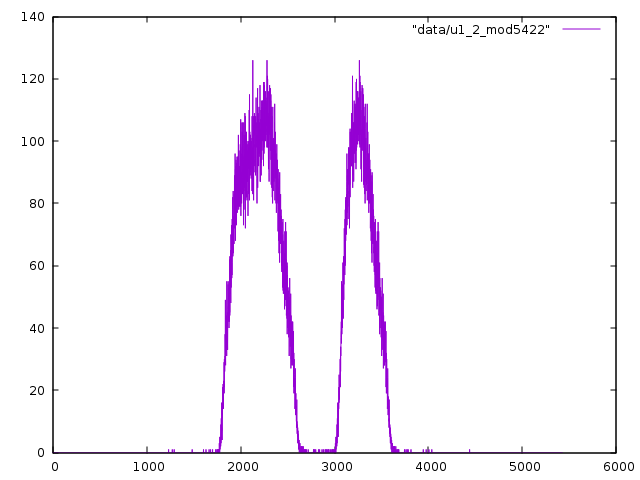
\includegraphics[scale=0.5]{../figs/u1_2_mod5422.png}
\end{center}
\end{figure}

This has some notable features: 

\begin{itemize}
\item From the value of $f_N(0)$, it looks like the Ulam
  sequence has small but nonzero density (in fact, around $0.07$).

\item As noted in \cite{steinerberger:preprint} it looks like as we increase $N$
  that this is converging to an actually continuous distribution.

\item It looks at a glance like this distribution is supported on the
  middle third of the interval $[0,\frac{2\pi}\alpha]$.  This is not
  literally the case, but in \cite{gibbs:preprint} there is a
  conjecture in this direction.
\end{itemize}

This phenomenon is actually apparent even after plotting a much
smaller number of Ulam numbers--say $10^3$, and does not appear to
weaken even after other people have computed many more Ulam numbers.

The striking nature and numerical strength of this phenomenon
naturally leads to many questions.  We will list a larger number of
these in section 3, but we give a sampling now: 

\begin{enumerate}
\item What is the $\alpha$ that appears to account for the entire
  spectrum of the Ulam numbers?  Is it irrational?  Transcendental?

\item What feature of the Ulam numbers gives rise to this
  distribution?  For example, can we write down a general class of
  sets with this behaviour?

\item What is it that causes some initial conditions to be regular and
  not others (if indeed they are not)?

\item Can we distill this phenomenon into a more general notion of
  regularity that even the irregular-looking sequences do satisfy?
\end{enumerate}

\subsection{Notation}

Before we get to our results, we provide a few pieces of notation that
we shall use throughout this document: 

\begin{itemize}
\item Denote by $[N]$ the set $\{1, \ldots, N\}$.
\item If $A \subseteq \N$, let $A_N$ denote $A \cap [N]$.  
\item If $f(N)$ is a function: 
\begin{itemize}
\item $f$ is $\O(g(N))$ if there is a constant $C > 0$ such that $f(N)
  \leq C g(N)$ for $N$ sufficiently large.
\item $f$ is $\Omega(g(N))$ if there is a constant $C > 0$ such that
  $f(N) \geq C g(N)$ for $N$ sufficiently large.
\item $f$ is $\Theta(g(N))$ if there are constants $C, C' > 0$ such
  that $C g(N) \leq f(N) \leq C' g(N)$.
\end{itemize}
\item For $x \in \R$, let $e(x)$ denote $e^{ix}$.
\end{itemize}

\section{Results}

In this document, we do not provide a complete explanation for the
phenomenon, but we do focus attention on a class of sets that all seem
to exhibit simlar behaviour, namely ``\relevant sets'': The idea is
that the set $A$ of Ulam numbers has the property that the number of
pairs $(x, y) \in A^2$ with $x + y \in A$ is unusually small.  For
example, in a randomly generated set $B$ of density $\delta$, we might
expect that $B_N$ has about $\delta N$ elements, and hence
$\delta^2 N^2$ pairs of elements.  Of these pairs, we expect $\delta$
to be the proportion of them whose sums are also in $A$.  That is, we
expect about $\delta^3 N^2$, or, generally, $\Theta(N^2)$ solutions to
$x + y = z$ with all $x, y, z \in A$.  If we have fewer of these, say
$O(N^{2-\epsilon})$ for some $\epsilon > 0$, then that would suggest
that the set cannot be purely random.  So we define:

\begin{definition}Call a set $A$ of positive integers
  \textbf{\relevant}if there is a constant $C \geq 0$ and
  $\epsilon > 0$ such that if
  $T(A_N) = |\{(x, y)\in A_N^2 : x + y \in A_N\}|$, then
  $T(A_N) \leq C N^{2-\epsilon}$ for all $N$.
\end{definition}

\begin{example}
  Any $(a,b)$-Ulam sequence is \relevant because for each Ulam number
  $x < N$, the number of representations $x$ has as a sum of other
  Ulam numbers is at most 3: The sum that qualifies it to be an Ulam
  number in the first place, that same sum with the order reversed,
  and possible $\frac{x}{2} + \frac{x}{2}$ if $\frac{x}{2}$ happens to
  also be in the sequence.  Thus such a sequence has $T(A_N) \leq 3N$,
  and thus is \relevant with $C = 3$ and $\epsilon = 1$.
\end{example}

\begin{example}
  A set $A$ is called ``sum-free'' if for every $N$, $T(A_N) = 0$.
  These sets are thus also \relevant and indeed will provide examples
  of the same phenomena that are in some ways simpler and more extreme
  than the Ulam numbers.
\end{example}

As we discussed above, these sets are defined in a way that guarantees
they behave differently from truly random sets.  One might wonder,
then, what structure this definition actually guarantees for such
sets.

We suspect that the nature of this structure is roughly ``correlation
with a periodic sum-free set''.  More precisely, that there should be
a $\lambda \in \R$ such that if $\pi : \R \to \R/\Z$ is the map
$x \mapsto \lambda x\mod{1}$, then there is an actually sum-free
subset $E \subseteq \R/\Z$ such that $A$ and $\pi\inv(E)$ are in some
sense strongly correlated.

In this document, we come to a first result in this direction: theorem
\ref{thm:regularity}, which gives such a $\lambda$ and a set
$E \subseteq \R/\lambda\Z$ that is ``more correlated than expected''
with $A$.  We also show (theorem \ref{thm:regular_sumfree}) that
regular Ulam sequences are eventually equivalent to lifts of a
sum-free subset of some $\Z/m$.

To get such results, we first prove a theorem (theorem
\ref{thm:alpha_finitary}) that \relevant sets are guaranteed (in a
certain sense) a large Fourier coefficient $\alpha$ in their spectrum.
We also show in theorem \ref{thm:hole1}, granting certain statements
about the Fourier spectrum that we could not prove, that certain
features of this distribution should follow from arguments in the vein
of the circle method.

Finally, turning our attention from the general study of \relevant
sets to the Ulam numbers in particular, we consider the combinatorial
structure of the Ulam numbers that results from their definition.  For
example, we know that every Ulam number $a$ has a unique pair of Ulam
numbers $x < y$ with $x + y = a$.  We can ask questions about the
distribution of such $x$ and $y$--for example, does every Ulam number
show up as a summand of other Ulam numbers equally often?  Further,
$x$ and $y$ are also Ulam numbers so they can be decomposed likewise
until every $(u,v)$-Ulam number is expressed as a sum of $u$s and
$v$s.  The distributions of these also makes for interesting study.
And lastly, we might ask what kind of structure would give rise to an
``irrationally regular'' sequence with the additive structure that the
Ulam numbers have.  To this end, we propose in proposition
\ref{prop:irr_1add} a construction that is not regular in the earlier
sense, but that does have some non-trivial irrational periodicity.

\chapter{Background}

We will start by giving an overview of some known results that should
lead us in the right direction.  No arguments in this section are
original.

\section{Fourier Transform}

The definition of the Fourier transform-like operator that seems
experimentally to be the one that applies is the following:

\begin{definition}\label{def:fourier}
For $A \subseteq \Z^+$ a set of positive integers, define for any
$x\in \R/2\pi\Z$: 

\[\widehat{A_N}(x) = \frac{1}{N} \sum_{t=0}^{N-1} A(x) e(tx)\]

Also define

\[\widehat{A}(x) = \lim_{N \to \infty} \widehat{A_N}(x)\]
if this limit converges.  
\end{definition}

So, for example, if $A$ is the Ulam numbers, $\widehat{A}(0)$ would be
the so-called natural density $\delta$ (which may be around $0.07$) if
it exists.  Then the observation of Steinerberger is that
$\widehat{A}(x) = 0$ unless $x \in \alpha\Z$ for the above particular
choice of $\alpha$, and
$\widehat{A}(\alpha) \approx 0.8\delta \approx 0.056$, for example.

Of course, it is not clear that this definition ever converges or what
properties it might satisfy, so we shall in this document always work
only with truncated sequences $A_N \subseteq [N] = \{1, \ldots, N\}$,
where we can view $[N]$ as $\Z/N$ and apply a more standard
definition:

\begin{definition}
  For $f : \Z/N \to \C$, let the \textbf{discrete Fourier transform}
  of $f$ be a function $\dft_N f$ defined for $k \in \Z/N$ by:
  \[(\dft_N f)(k) = \frac{1}{N} \sum_{t=0}^{N-1} f(t) e(-\frac{2\pi k t}{N})\]
\end{definition}

This definition satisfies many properties, which are standard from
Fourier analysis and additive combinatorics \cite{tao:cup2006}:

\begin{proposition}\label{prop:fourier}
If $f : \Z/N \to \C$, then: 

\begin{itemize}
\item If in fact $f$ takes values in $\R$, then
  $(\dft_N f)(-x) = \overline{(\dft_N f)(x)}$ for all $x \in \Z/N$.

\item If in fact $f$ is the indicator function of a set
  $A \subseteq \Z/N$ with $|A| = \delta N$, then
  $(\dft_N f)(0) = \delta$, and $|(\dft_N f)(x)| \leq \delta$ for all
  $x \in \Z/N$.

\item (Fourier inversion): $(\dft_N\inv f)(x) = N (\dft_N f)(-x)$ for
  all $x \in \Z/N$.

\item (Convolution formula): For two functions $f, g : \Z/N \to \C$,
  we have \[(\dft_N (f \ast g))(x) = N(\dft_N f)(x)(\dft_N g)(x)\] for all
  $x \in \Z/N$, where $(F \ast G)(x) = \sum_{t=0}^{N-1} F(t)G(x-t)$ is
  the convolution of $F$ and $G$.

\item (Cross-correlation formula): For two functions
  $f, g : \Z/N \to \C$, we have
  \[(\dft_N (f \star g))(x) = N(\dft_N f)(-x)(\dft_N g)(x)\] for all
  $x \in \Z/N$, where $(F \star G)(x) = \sum_{t=0}^{N-1} F(t)G(t+x)$
  is the cross-correlation of $F$ and $G$.

\item (Parseval's identity): For $f : \Z/N \to \C$, we
  have
  \[\sum_{t=0}^{N-1} |(\dft_N f)(t)|^2 = \frac{1}{N} \sum_{t=0}^{N-1}
    |f(t)|^2\]
\end{itemize}
\end{proposition}

\section{Known regularity results}

If we want to prove some kind of generalised regularity statement, it
might help to understand existing proofs of regularity (i.e. that
consecutive differences are eventually periodic) in cases where this
is known to hold.  We discuss two such results in this section.

\subsection{Finch's criterion for regularity}

In \cite{finch:em1992}, Finch proves:

\begin{theorem}
  If $A = U(a,b)$ is an Ulam sequence containing finitely many even
  elements, then $A$ is regular.
\end{theorem}

The idea of the proof is that if there are finitely many evens, say
$e_1 < \ldots < e_s$, then every term $n$ after the last even must be
odd.  Since it can be written as sum of two earlier terms, and it is
odd, one of its summands must be even.  And since it can be written in
such a sum in a unique way, this is saying that $n - e_i$ is in the
sequence for a unique $i$ from 1 to $s$.  This is finitely many things
to check, from which regularity should follow.

More precisely:

\begin{proof}

  If $x_n$ is the number of representations of $n$ as a sum of two
  elements of $A$ and $n$ is odd, then because an odd number that is a
  sum of two smaller elements of $A$ must have an even summand and we
  have only finitely many evens $e_1 < \ldots < e_s$, we can write a
  finite recurrence:

  \[x_n = \sum_{i=1}^s 1(x_{n-e_i})\]
  where $1(x)$ is 0 unless $x = 1$, in which case $1(x) = 1$.  In
  particular, $0 < x_n \leq s$ for all odd $n > e_s$.  Note also that
  $x_n$ depends on a finite range of earlier $x_i$'s:
  $x_{n-2}, x_{n-4}, \ldots, x_{n-e_s}$.  Call this sequence $B_n$.
  Each of the $e_s/2$ values in $B_n$ is between 1 and $s$, so there
  are finitely many possible such sequences.  Thus, for some $N$ and
  $n$, we must have $B_n = B_{n+N}$.  But since $x_n$ and $x_{n+N}$
  only depend on $B_n$ and $B_{n+N}$ respectively, this means
  $x_n = x_{n+N}$.

  And further, $x_{n+2}$ and $x_{n+N+2}$ only depend on the sequences
  $B_{n+2}$ and $B_{n+N+2}$, respectively.  But 

  \begin{eqnarray*}
    B_{n+N+2} &=& (x_{n+N}, x_{n+N-2}, \ldots, x_{n+N+2-e_s}) \text{
    by definition}\\
    &=& (x_{n+N}, x_{n-2}, \ldots, x_{n+2-e_s}) \text{ because $B_n
                                                  = B_{n+N}$}\\
    &=& (x_{n}, x_{n-2}, \ldots, x_{n+2-e_s}) \text{ as noted
                                                above}\\
              &=& B_{n+2}
  \end{eqnarray*}

  So in fact $B_{n+N+2} = B_{n+2}$ and we can proceed by induction to
  show the $B_n$ are periodic with period $N$.  Since the $x_n$ are
  determined by the $B_n$, $x_n$ is therefore also periodic with
  period $N$.
\end{proof}

Using numerical computations inspired by this criterion, Finch
conjectures \cite{finch:em1992} that the following $U(a,b)$ are
regular:

\begin{conjecture}[Finch]
  $U(a,b)$ has only finitely many even terms if and only if $(a,b)$ is
  in the following list:

\begin{itemize}
\item $(5,6)$.
\item $(2,v)$ for $v \geq 5$ and odd.
\item $(u,v)$ for $u \geq 4$ and even.
\item $(u,v)$ for $u \geq 7$ and odd if $v$ is even.
\end{itemize}
\end{conjecture}

In particular this would imply that all of these sequences are
regular, although the above may not be the complete list of regular
$U(a,b)$.

\subsection{Regularity of $U(2,2n+3)$}

Using the above criterion, Schmerl and Speigel in
\cite{schmerl:jct1994} prove:

\begin{theorem}
  The sets $U(2,v)$ for $v > 5$ and odd are regular.
\end{theorem}

Since they use Finch's criterion, this boils down to showing that each
of these sets has finitely many evens.  Specifically: 

\begin{lemma}The only even elements in the 1-additive set $U(2,v)$
  (with $v > 5$ odd) are 2 and $2v+2$.
\end{lemma}


\begin{proof}
  The proof goes by supposing that $x$ is the next even element of
  $U(2,v)$ after $2v+2$ and using an exhaustive knowledge of small
  elements of the sequence (up to about $5v$) to write $x = a+b$ for
  smaller $a, b \in U(2,v)$ in more than one way.  To do this, we have
  to understand the small elements of the sequence and the elements
  just before $x$.  

  We leave out the computation of the small elements and simply state
  the result: 

  \begin{lemma}
    The elements of $U(2,v)$ up to $5v+10$ are: 

    \begin{itemize}
      \item $2$
      \item $2v+2$
      \item All odds between $v$ and $3v$, inclusive.
      \item $3v+4i$ for $0 < i \leq \frac{v+1}{2}$ (that is, every
        other odd from $3v$ to $5v+2$ inclusive)
      \item $5v+4$
      \item $5v+10$
    \end{itemize}
  \end{lemma}

  To use these to express our supposed next even element $x$ as a sum
  of elements of $U(2,v)$ in multiple ways, we also need to understand
  the elements immediately leading up to $x$.  

  \begin{lemma}
    There is no gap of length $2v$ in the odd numbers in the sequence
    up to $x-2v$.  More precisely, if $r$ is any odd number less than
    $x-2v$, then one of $r, r+2, \ldots, r+2v$ is in $U(2,v)$.  
  \end{lemma}
  \begin{proof}
    If we take $r$ to be the minimal counterexample to this, then $r-2$
    is in $U(2,v)$, else $r-2$ would be a smaller counterexample (note
    that 1 is manifestly not a counterexample, so $r-2 > 0$).  

    But then $r+2v = (r-2)+(2v+2)$ expresses $r+2v$ as a sum of
    elements of $U(2,v)$, so the only way it can fail to be in
    $U(2,v)$ is if there is another such expression.  But $r+2v$ is
    odd, so any other expression of it as $a+b$ for $a, b \in U(2,v)$
    requires that one of $a$ and $b$ be even.  And $r+2v < x$, so the
    only choice other than $2v+2$ (which we have already used) is 2.
    So this means $r+2v = 2+(r+2v-2)$ is the other such expression.
    But for this to be such an expression, $r+2v-2$ must be in
    $U(2,v)$, and we are done.
  \end{proof}

  \begin{corollary}
    It follows from the proof that for any odd $r < x-2v$
    $r \in U(2,v)$ if and only if exactly one of $r+2v+2$ and $r+2v$
    is in $U(2,v)$.
  \end{corollary}

  This will allow us to, for example, find several elements of
  $U(2,v)$ between $x-3v$ and $x$.  We already know that we have a lot
  of elements between $v$ and $3v$, so this gives us a good chance of
  expressing $x$ as a sum of elements of $U(2,v)$ in multiple ways.  

  For example, the second lemma tells us that some odd between $x-3v$
  and $x-v$, say $x-v-2i$ (for some $0 \leq i \leq v$) is in $U(2,v)$.
  But we know everything of the form $v+2i$ with $0 \leq i \leq v$ is
  in $U(2,v)$ as well, so \[x = (x-v-2i)+(v+2i)\] is the qualifying
  expression for $x$ as a sum of smaller elements.  Since this
  expression must be unique, we also know that $x-v-2j$ for
  $0 \leq j \leq v$ and $j \neq i$ cannot be in $U(2,v)$.

  To get a second such expression (and therefore a contradiction), we
  will look also at the odd elements from $x-5v$ to $x-3v$, using our
  knowledge of the odd elements of $U(2,v)$ from $3v$ to $5v$.  

  After some casework, this will end up giving a second qualifying
  expression for $x$, thereby disqualifying it.  We refer to
  \cite{schmerl:jct1994} for the details.
  
  % We shall look at these elements by considering
  % $y_k = (x-v-2k) - (2v+2)$.  By the corollary, $y_k$ is in $U(2,v)$
  % if and only if exactly one of $y_k+2v+2 = x-v-2k$ and
  % $y_k+2v = x-v-2(k+1)$ is in.  But this only happens if $k = i$ or
  % $k+1=i$, so the only elements in $x-3v$ to $x-5v$ that are in
  % $U(2,v)$ are $x-3v-2i-2$ and $x-3v-2i$.  

  \end{proof}

\section{Sum-free sets}

The set of Ulam numbers $A$ has the property that for each $a \in A$,
there is exactly one solution to $x+y=a$ with $x < y$ in $A$.  The
condition that $x < y$ is a little hard to capture using standard
techniques, but, for example, this entails that the number of
solutions to $x + y = a$ with $x, y \in A$ is at most 3 (namely, the
unique solution $x+y = a$ above, then also $y+x = a$, and then at most
one other solution of the form $z+z = a$, since the definition of the
Ulam numbers does not consider this.  For example, 4 is Ulam, and its
unique representation is $1+3=4$, but it also happens that $2+2=4$ and
2 is also Ulam).

In particular, this implies that if $A_N$ is again the set of Ulam
numbers up to $N$, then $A_N$ has at most $3|A_N|$ solutions to $x+y =
z$ with $x, y, z \in A_N$.  

In the interest of understanding what precisely is happening with the
Ulam numbers, then, we might turn our attention to the more extreme
situation of sets with no solutions to this equation at all: So-called
``sum-free sets''.  

\begin{definition}
  A subset $A$ of an abelian group is \textbf{sum-free} if the
  equation $x+y=z$ has no solutions with $x, y, z \in A$.
\end{definition}

\begin{example}
\begin{enumerate}
\item The odd positive integers are sum-free.  
\item More generally, if $A \subset \Z/m$ is sum-free, then the set of
  integers $x$ that reduce to an element of $A$ modulo $m$ is also
  sum-free.  
\item Even more generally, for any homomorphism $\pi : \Z \to \R/\Z$,
  if $A$ is a sum-free subset of $\R/\Z$, then $\pi\inv(A)$ is a
  sum-free set of integers.
\item Any subset of a sum-free set is sum-free also.
\end{enumerate}
\end{example}

When we think about generalising the particular notion of
``regularity'' above for the purpose of the Ulam sequence or for
sum-free sets, the basic thought is that a set should be ``regular''
in a more general sense if it has some non-trivial correlation with a
set of the form in example 3.

\subsection{Decision sequences}

It turns out there is a construction that bijects sum-free sets of
positive integers with infinite binary sequences.  In words, the
construction is simple: Take the positive integers in turn starting
with 1.  For each integer, flip a coin.  If the coin shows heads,
include that integer in the set and erase all integers that are sums
of pairs of elements in the set thus far (as these cannot be in the
set if the set is to be sum-free).  If tails, do not include that
integer in the set.  Then move on to the next integer that has not
already been included, excluded by a ``tails'' result, or disqualified
by being erased.

More formally: 

\begin{definition}Define the function
  $\theta : \{0,1\}^\N \to \{f : \N \to \{0,1\}\}$ from binary
  sequences to sum-free sets of natural numbers (or, in this case,
  their indicator functions) as follows: If $s\in\{0,1\}$ is a binary
  sequence, then using $s$, we will actually define three disjoint
  sets that partition the natural numbers: The target set $A$, the
  excluded set $E$, and the disqualified set $D$.  For each
  $n \in \N$, iteratively select a set for $n$ as follows:
\[\begin{cases}
n \in A+A &\implies n \in D\\
n \notin A+A \text{ and } s_k = 1 &\implies n \in A\\
n \notin A+A \text{ and } s_k = 0 &\implies n \in E
\end{cases}\]
where, at each stage, $k = |A|+|E|+1$ is the index of the first
element of $s$ that we have yet to consult. 

If $S$ is a sequence and $A$ is a sum-free set with $\theta(S) = A$,
then $S$ is called the \textbf{decision sequence} for $A$.
\end{definition}

\begin{example}
  For example, let us compute $\theta(111111111...)$: We start with 1
  and flip a coin and get heads, so we include 1 in the set $A$.  This
  automatically disqualifies 2 as $2 = 1+1$.  The next possible
  candidate is 3, so we flip another coin and get heads, and so we
  include 3.  This automatically disqualifies 4 ($4 = 1+3$) and 6
  ($6 = 3+3$).  Continuing in this way, it is clear we will never get
  a chance to include an even number and will always include the odd
  numbers, so in the end, the result is the set of odd positive
  integers.
\end{example}

It is also possible to reverse this construction.  In words: Say we
start with $A$ a sum-free set.  We again walk through the positive
integers starting at 1.  For each $n$ there are three possibilities:
Either $n \in A$, $n \in A+A$, or neither.  If $n \in A$, then it got
there by a coin landing heads, so we write down a 1.  If $n \in A+A$,
then $n$ was disqualified from being in $A$ not by a coin flip, but by
being a sum of elements of $A$, so we write down nothing.  If $n
\notin A$ and also $n \notin A+A$ then $n$ could have been included in
$A$, but was excluded simply because of a coin flip, so we write down
a 0.  

Formally, we write down the sequence $s = \theta\inv(A)$ by writing
down first the string $s'$ whose $n$th character is: 

\[s'_n = \begin{cases}
\text{`A'}& \text{if } n \in A\\
\text{`D'}& \text{if } n \in A+A\\
\text{`E'}& \text{if } n \notin A \cup (A+A)
\end{cases}\]

(So all the `A's are elements of $A$, all the `D's are automatically
excluded from $A$ by being sums of prior elements of $A$, and all the
`E's are things that are excluded from $A$ despite the fact that their
inclusion would not violate the sum-free property.)  Then the decision
sequence $s$ of $A$ is got by starting with $s'$ and deleting all
$D$s, replacing all $A$s with 1, and replacing all $E$s with 0.

There are many questions about this construction.  For example, it is
known that if a sum-free set $A$ is regular (as defined
above--i.e. its sequence of successive differences is ultimately
periodic), then its decision sequence $\theta\inv(A)$ must also be
ultimately periodic \cite{cameron:sc1987}.  Conversely, many periodic
decision sequences give rise to provably regular sum-free sets.  For
example, say for a finite string $s$ that $\overline{s}$ denotes the
infinite string got by repeating $s$ forever.  Then all $s$ of length
five are known to have $\theta(\overline{s})$ regular except
$s = 01001$, $s = 01010$, and $s = 10010$.  For example,
$\theta(\overline{01001})$ (which we will somewhat abusively refer to
as $\theta(01001)$) starts
$\{2, 6, 9, 14, 19, 26, 29, 36, 39, 47, 54, 64, 69, 79, 84, 91, 96,
\ldots\}$ and has been computed extensively with no period being
identified to date.  Beyond the failure of brute force attempts to
find a period for it, there is other computational evidence in
\cite{calkin:int2005} that this sequence may not be periodic.
Nevertheless, there is no known example of an ultimately periodic
decision sequence for which we can actually prove its corresponding
sum-free set is non-regular.

\subsection{Density and regularity}

In the world of sum-free sets, the odd integers provide an example of
a very large sum-free set.  In fact, a theorem of Luczak that we will
discuss in this section shows that they are the largest example: Any
sum-free set that has an even number has density bounded by $\frac25$.
Before we can discuss this, however, we will dwell for a brief moment
on what we mean by ``density'':

\begin{definition}
  A subset $A \subset \Z^+$ has \textbf{density} $\delta$ if
  $\lim_{N \to \infty} \frac{|A_N|}{N}$ exists and is equal to
  $\delta$.
\end{definition}

Since this may not always exist, we might work with another quantity
that will always exist and that, in cases when the density does not
exist, provides what should be thought of as at least an upper bound:

\begin{definition}
  A subset $A \subset \Z^+$ has \textbf{upper density} $\delta$ if
  $\limsup_{N \to \infty}\frac{|A_N|}{N} = \delta$.
\end{definition}

As we have noted, then, the maximal upper density a sum-free set can
have is $\frac12$, which is realised by the example of the odd
positive integers.  Luczak has given a sort of converse to this
example, proving in \cite{luczak:jct1995} the following: 

\begin{theorem}[Luczak]
If $A$ is a sum-free set of positive integers and there is at least
one even integer in $A$, then the upper density of $A$ is bounded
above by $\frac25$.  
\end{theorem}  

The proof is short, but a
little delicate, and we shall recall a version of it in this section.

The basic idea of the proof is to find disjoint subsets of $[N]$ that
are the same size as $A_N$, or of a size related to $A_N$.  For
example, if $a \in A_N$ is any element, then because $A$ is sum-free,
$A_N$ and $A_N+a$ are disjoint in $[N+a]$, but have the same size, and
thus $2|A_N| \leq N+a$, i.e. $|A_N|/N \leq \frac12 + \frac{a}{2N}$.
Taking the limit as $N \to \infty$, we again deduce our earlier
statement about $A$ having density bounded by $\frac12$.

\begin{proof}
Note first that if $A$ is all even elements, then $\frac12 A$ is
also sum-free, and therefore with density $\leq \frac12$, and so $A$
has density $\leq \frac14$ and the result is automatic, so without
loss we may assume $A$ has at least one odd element in addition to its
at least one even element.  

With this in mind, the proof breaks up into two cases: Where $A$
contains consecutive elements and where it does not.

\textbf{Case 1: $A$ has no consecutive elements} In the case where $A$
has an even element but no two consecutive elements, let $t$ be the
minimal odd positive element of $A-A$ which does exist (using the fact
that $A$ has both odd and even elements), and is not 1 (since there
are no consecutive elements).  Also fix $x, y \in A$ with $t = x-y$.

This means that if $a \in A$, then $a+t-2$ cannot be in $A$ (else
$t-2$ would be a smaller odd positive difference than the minimal odd
difference $t$).  Put another way, if $a$ and $a+2$ are both in $A$,
then $a+t$ cannot be in $A$.  Put another way, if $B$ is the set of
$a \in A$ with $a+2$ also in $A$, then $B+t$ and $A$ are disjoint.  Of
course, we already know that finding two disjoint subsets of size even
as large as $|A|$ is already easy, however this lets us in fact find
three: Since $t=x-y$, this means $B+x-y$ and $A$ are disjoint, meaning
$B+x$ and $A+y$ are disjoint.  But both of these are contained in
$A+A$, so they are both also disjoint from $A$.  Thus we have $A$,
$A+y$, and $B+x$ all disjoint.  If we truncate $A$ to $A_N$, then
$A_N$, $A_N + y$, and $B_N + x$ are all disjoint subsets of $[N+x]$,
and so

\[2|A_N|+|B_N| \leq N+x\].

So if we can relate $|B|$ to $|A|$ (for the moment using the shorthand
$B = B_N$, $A = A_N$), then we are done.  

But by the definition of $B$, we have two cases for an element of $A$: 
\begin{itemize}
\item $a \in B$, in which case $a+1$ is not in $A$.  
\item $a \in A\setminus B$, in which case we know $a+1$ is not in $A$
  (since $A$ has no consecutive elements) and $a+2$ is not in $A$,
  (since otherwise $a$ would be in $B$).
\end{itemize}

So we have the five sets:
$B, B+1, A\setminus B, (A\setminus B) + 1, (A\setminus B) + 2$, and
these are all pairwise disjoint in $[N+2]$.  (The only one that might
not be clear is $(B+1) \cap ((A \setminus B) + 2)$, but if
$a \in A\setminus B$ and $b \in B$ with $a+2=b+1$, then $a + 1 = b$,
giving two consecutive elements of $A$ which does not happen.)

Thus $2|B_N| + 3(|A_N| - |B_N|) \leq N+2$, i.e.

\[|B_N| \geq 3|A_N| - N - 2\]

Now we have a relationship between $|B|$ and $|A|$, so we can pair
this with our earlier inequality relating the two of them to $N$ and
find:
\[2|A_N| + 3|A_N| - N - 2 \leq N+x \]
or 
\[\frac{|A_N|}{N} \leq \frac25+o(1) \]
as we wanted.

\textbf{Case 2: $A$ has consecutive elements:} In the case where $A$
has $d$ consecutive elements $a, a+1, \ldots, a+d-1$, say, the
argument is similar in flavour to the above, but the technical details
are all slightly different.  We will first need a $t$ to serve the
role of our $t$ in case 1.  But now, the minimal odd difference is
simply 1.  So we do something slightly different: This time, we let
$t$ be any positive element of $A-A$ for which $t+1, \ldots, t+d$ are
all not in $A-A$.  

\begin{lemma}Such $t$ does exist.\end{lemma}

\begin{proof}Since $a, a+1 \in A$, we know $1 \in A-A$.  Then let $t$
  be the maximum of $1, \ldots, a-1$ that is in $A-A$, so nothing from
  $t$ to $a-1$ is in $A-A$ (by definition), and nothing from $a$ to
  $a+d-1$ is in $A-A$ either (since these are all in $A$), so at least
  $d$ elements (and possibly more) immediately after $t$ are not in
  $A-A$).
\end{proof}

Again, write $t = x-y$ for some fixed $x, y \in A$.

We proceed broadly as before on the two-step plan: 

\begin{enumerate}
\item Find a set $B$ of elements that gives rise to many disjoint
  subsets of $[N]$ and deduce a bound relating $|A_N|$ and $|B_N|$ to
  $N$.
\item Upper-bound $|B_N|$ in terms of $|A_N|$ and $N$, and plug this
  into the previous bound to get a bound on $|A_N|$ in terms of $N$.
\end{enumerate}

\textbf{Step 1: }Let $B$ be the set of elements $b$ for which
$b+1, \ldots, b+d-1$ are all not in $A$.  Then certainly the sets
$A, B+1, \ldots, B+d-1$, are all disjoint.  In fact, we can get one
more than this: We can shift all these sets by $a$ and they are still
disjoint: $A+a, B+a+j$ ($j=1, \ldots, d-1$).  But now since the $a+j$
are all in $A$, these sets are all themselves disjoint from $A$ (since
they are all subsets of $A+A$).  Thus, again truncating at $N$, we
have two sets of size $|A_N|$ and $d-1$ sets of size $|B_N|$ all
disjoint and inside $[N+a+d-1]$.  Thus:

\[2|A_N|+(d-1)|B_N| \leq N+a+d-1\]

\textbf{Step 2: }So again, we need control over the size of $|B_N|$ in
terms of $|A_N|$ and we will be done.  But this time, we note that if
$z \in A$, it is possible that $z+t$ could be in $A$, but that then
because of the definition of $t$, none of $z+t+1, \ldots, z+t+(d-1)$
can be in $A$ (lest one of $t+1, \ldots, t+(d-1)$ lie in $A-A$).  Thus
elements of $A+t$ that lie in $A$ in fact must lie in $B$.  Put another
way, $A+t$ and $A \setminus B$ are disjoint.  Again, this is only two
sets, but we can use the same trick as before to make it three: Since
$t = x-y$, we can equally say $A+x$ and $(A \setminus B) + y$ are
disjoint, at which point these are also disjoint from $A$ (again,
being subsets of $A+A$).  So we have three disjoint subsets $A+x$,
$A \setminus B + y$, and $A$ of $[N+x]$, with sizes $|A_N|$, $|A_N|$,
and $|A_N|-|B_N|$, respectively.  This gives
$|A_N| + |A_N| + (|A_N| - |B_N|) \leq N+x$ or:

\[|B_N| \geq 3|A_N|-N-x\]

Dropping this into the first inequality and rearranging, we get:

\[2|A_N|+(d-1)(3|A_N|-N-x) \leq N+a+d-1\]
which simplifies to: 
\[\frac{|A_N|}{N} \leq \frac{d}{3d-1} + o(1)\]

Since $d \geq 2$ (as we are assuming we have at least two consecutive
elements), this is again bounded by $\frac25$ in the limit, so the
claimed bound follows.
\end{proof}

\subsection{Aperiodic sum-free sets}

A construction of Erdos in \cite{erdos:spm1965} supplies an example of
a sum-free set with density $\frac13$ that is provably not regular,
namely: Take $\alpha \in \R$ irrational, and let $A_\alpha$ be the set
of integers $n$ such that $n \mod{\alpha}$ lies in
$\left(\frac \alpha 3, \frac {2\alpha}{3}\right)$.  $A_\alpha$ is
clearly sum-free, since it is sum-free modulo $\alpha$, but for
irrational $\alpha$, $A_\alpha$ is also not periodic.  That is, for
every modulus $m$ and every residue class $k$, there is an element of
$A_\alpha$ congruent to $k$ mod $m$.

Indeed, equidistribution results for irrational numbers tell us that
there the integers are equidistributed modulo any irrational.  For
example, there is at least one $n$ that is equivalent to an integer in
the interval $\left(\frac{\alpha}{3m}-k,\frac{2\alpha}{3m}-k\right)$
modulo the irrational number $\frac{\alpha}{m}$.  Then it is clear
that $mn+k$ will reduce to an element of
$\left(\frac{\alpha}{3},\frac{2\alpha}{3}\right)$ mod $\alpha$,
meaning that $mn+k \in A_\alpha$ as desired.

%\section{Abelian arithmetic regularity}

% If $A$ is any set, then an easy probablistic argument shows that there
% is a sum-free subset of $A$ of size $|A|/3$.  Indeed, if for any real $\alpha$,
% we define $A_\alpha$ to be set the set of elements $x$ of $A$ with

% \[A_\alpha = \{x \in A : 1/3 < \alpha x \mod{1} \leq 2/3\]

% then the expected size of $A_\alpha$ is $|A|/3$ as $\alpha$ varies
% over $[0,1]$, and so there must be at least one a for which $A_\alpha$
% has at least this size.

% In \cite{no_large_sumfree_subset_eberhard} prove that for every e > 0, there is a set A such
% that A has no sum-free set larger than $(1/3 + \epsilon)|A|$, so this
% bound is in fact sharp (to first order).  (Apropos of nothing, I find
% this paper's organisation and general exposition to be highly
% user-friendly and otherwise excellent.)

% In our case, if $A$ is the Ulam sequence up to N, then for any
% $\epsilon > 0$ we believe that for $N$ large enough, we could generate
% a sum-free subset of size $(1-\epsilon)|A|$--kind of the opposite
% extreme.

% Nevertheless, the argument follows a kind of local-to-global flow that
% might make it worth understanding, so we work through at least the
% basic idea here:

% ...

%}

\section{Roth's theorem}

Roth's theorem is about the number of 3-term arithmetic progressions
$x, y, z$ in a set $A \subseteq \Z^+$.  Specifically: 

\begin{theorem}[Roth's theorem]
  Let $A \subseteq Z^+$ be a set of positive integers with positive
  upper density.  Then $A$ contains infinitely many arithmetic
  progressions $a, a+d, a+2d$ of length 3.  
\end{theorem}

Equivalently, such an $A$ always has at least one solution to $x+z=2y$
(whereupon $x, y, z$ is an arithmetic progression of length $3$).  A
sum-free set $A$ instead has are no solutions to $x+z=y$ (swapping
around variable names to highlight the similarity), so if we have a
sum-free set that we believe has positive density, we might wonder
what the proof of Roth's theorem has to say about it.  (After all, in
the case of the slightly different equation $x+z=2y$, it says that the
set $A$ cannot exist.)

As it turns out, many new techniques in additive combinatorics cut
their teeth on Roth's theorem, and so there are many proofs, from
those that use probabilistic techniques to ergodic theory.  We will
discuss one in particular: The density increment proof.  We will not
give the complete proof, but will simply work at a high level through
the part that is relevant to our study and will outline the rest.

\subsection{Density increment proof}

Proofs of Roth's theorem often work with a finitary version of the
statement, which we make now:

\begin{theorem}[Roth's theorem]
  For every $\delta > 0$, there is an $N_0 > 0$ such that for every
  $N > N_0$, every $A \subseteq [N]$ with $|A| > \delta N$ contains a
  solution to $x+z=2y$.
\end{theorem}

One strategy of proof goes via Fourier analysis, saying that if $A$
has no large Fourier coefficients, then $A$ is guaranteed to behave
``pseudorandomly'' in some sense, and computes that such sets must
automatically have many length-3 arithmetic progressions, and we are
done already.  

If, on the other hand, $A$ does have some large Fourier coefficient,
then one can find a long arithmetic progression that has large
intersection with $A$, and on which $A$ in fact has higher density
than it had originally.  We can repeat this step (the ``density
increment'') as often as needed until either our intersected $A$ has
no large Fourier coefficient (in which case we are done as before) or
else $A$'s density in the arithmetic progression increases to 1.  And
if we are careful about it, we can ensure that at least 3 elements
will still remain by the time we get to this point.

\begin{proof}[Proof of Roth's theorem via density increment]

  Rather than working on the set $[N]$, we shall work with the group
  $\Z/N$, noting that if $A$ only contains elements smaller than
  $N/2$, then a solution to $x+z=2y$ in $\Z/N$ is an honest solution
  to $x+z=2y$ in $A$ viewed as a subset of $\Z$.  

  If $A$ is a set of density $\delta$ in $\Z/N$, with all elements of
  $A$ less than $N/2$, then the number $S$ of solutions to $x+z=2y$ is
  counted by:

  \[S = \sum_{x, y, z = 0}^{N-1}A(x)A(y)A(z)\delta_{x+y-z}\]

  Where $\delta_x = 1$ if $x = 0$, else $\delta_x = 0$.  Then, writing

  \[\delta_x = \frac{1}{N}\sum_{t=0}^{N-1}e(\frac{2\pi tx}{N}) =
    \widehat{1}\]

  we can substitute this into our expression for $S$ and rearrange,
  where for the sake of brevity (and only for the duration of this
  proof), we depart from our previous notation and denote by
  $\widehat{A}$ the discrete Fourier transform 

  \[\widehat{A}(x) = \frac{1}{N}\sum_{t=0}^{N-1}e(\frac{2\pi tx}{N})\]

  On doing so, we find:

  \[S = N^2 \sum_{t=0}^{N-1} \widehat{A}(t)\widehat{A}(t)\widehat{A}(-2t)\]

  The idea will be to pull out the $t = 0$ term of this sum, note that
  this is large and that if all other terms are small, than it
  dominates and guarantees $S > 0$.  Precisely:

  \begin{eqnarray*}
    S &=& N^2 \sum_{t=0}^{N-1} \widehat{A}(t)\widehat{A}(t)\widehat{A}(-2t) \\
    S &=& N^2 \delta^3 + N^2 \sum_{t=1}^{N-1} \widehat{A}(t)\widehat{A}(t)\widehat{A}(-2t) \\
      &=& \delta^3 N^2 + N^2 \sum_{t=0}^{N-1} \widehat{A}(t)^2\widehat{A}(-2t) \\
      &\geq& \delta^3 N^2 - \sup_t |\widehat{A}(-2t)| N^2 \sum_{t=0}^{N-1} |\widehat{A}(t)|^2 \\
      &=& \delta^3 N^2 - \sup_t |\widehat{A}(-2t)| N \sum_{t=0}^{N-1} |A(t)|^2 \\
      &=& \delta^3 N^2 - \sup_t |\widehat{A}(-2t)| N |A|\\
      &=& \delta^3 N^2 - \sup_k |\widehat{A}(k)| \delta N^2
  \end{eqnarray*}

  So if there is no large Fourier coefficient--that is, every Fourier
  coefficient is $\leq \epsilon N$, then
  
  \[S \geq (\delta^3 - \delta\epsilon) N^2\]

  In particular, if $\epsilon < \delta^2$, then $S > 0$, at which
  point there is at least one solution, as desired.
  
  If, on the other hand, there is a $k$ such that
  $|\widehat{A}(k)| \geq \delta^2 N$, then this argument does not
  guarantee a solution.  However, in that case, let $P = d[1,L]$ be
  the arithmetic progression of length $L$ and difference $d$
  $\{d, 2d, \ldots ,Ld\}$ ($d$ to be chosen later).  We want an
  arithmetic progression in which $A$ has higher density than it has
  in $\Z/N$ at large.  In other words, we want to find an $a$ that
  makes $Q(a) = |A \cap (P+a)| = (A \star P)(a)$ large.  But this we
  can analyse using Fourier analysis:
  
  \begin{eqnarray*}
    \widehat{Q}(s) = \widehat{A}(s) \overline{\widehat{P}(s)}
  \end{eqnarray*}
  
  Further, we know that for all $s \neq 0$,
  $\sum_a Q(a) \geq |\widehat{Q}(s)|$ (looking at the definition of
  the Fourier transform and using the triangle inequality).  So in
  particular, for $s = k$ (the large Fourier coefficient):

\begin{eqnarray*}
  \sum_a Q(a) &\geq& |\widehat{Q}(k)| \\
              &=& |\widehat{A}(k)| |\widehat{P}(k)| \\
              &\geq& \epsilon N |\widehat{P}(k)| 
\end{eqnarray*}

Thus for some $a$, $Q(a)/N \geq \delta^2 |\widehat{P}(k)|$.  We can
select $d$ and $L$ such that $|\widehat{P}(k)| \geq L/2$, so for some
$A$, $Q(a)/N \geq \epsilon L/2$.  In particular, $A$ intersected with
an arithmetic progression of length $L$ has density
$\delta + \epsilon/2$, meaning we have increased the density,
whereupon we can repeat the argument.

The details (such as actually selecting the correct $d$ and $L$, as
well as properly transitioning from $\Z/N$ back to $\Z$), are covered
in many places, for example \cite{roth:jlm1953}.

\end{proof}

% \subsection{Proof via the regularity theorem}

% The density increment proof exemplifies a kind of dichootomy between
% structure and randomness in its two cases: Where $A$ behaves
% pseudorandomly, in which density controls all the counting
% expressions, and where $A$ has structure, which we can use exploit to
% iterate the argument.

% The pseudorandomness argument will carry over nicely to the sum-free
% and Ulam cases, but second part of the argument relies on the fact
% that the structure of interest--in the case of Roth, arithmetic
% progressions, and in our case, additive triangles--can be found
% equally in any arithmetic progression.  For progressions, this is
% clear, but for triangles, this is simply false: The very dense
% progression of all odd numbers already contains zero additive
% triangles.  

% As this part of the proof seems unlikely to generalise to our
% situation, we explore a second avenue of proof for Roth's theorem,
% namely using the arithmetic regularity and counting lemmas of the
% earlier section.  This comes from \cite{tao:ams2012}

% \begin{proof}[Proof of Roth's theorem via arithmetic regularity]
%   For a function $f : [N] \to \{0,1\}$, define
%   $T(f) = \sum_{x,y \in [N]} f(x)f(x+y)f(x+2y)$ to be the function
%   that counts 3-term progressions if $f$ is thought of as an indicator
%   function.  So our goal is to prove that for $A \subseteq [N]$ of
%   density $\delta$ (for $N$ sufficiently large relative to $\delta$)
%   that $T(1_A) > 0$.  
  
%   As in the statement of the regularity lemma, write
%   $1_A = f_{str} + f_{sml} + f_{unf}$ with parameters $M$ and
%   $\epsilon$.  .
% \end{proof}

% %\section{Green's arithmetic triangle removal theorem}
% }

\section{Quantitative bounds in finite fields}

There have been several recent developments in a finite field setting
on analogous problems (specifically, the work of Croot, Lev, and Pach
\cite{croot:preprint} on length-3 arithmetic progression-free sets in
$\FF_4^n$ and subsequent work by others \cite{ellenberg:preprint}
pushing it to $\FF_3^n$).

We will recall the method used here by outlining the proof in
\cite{ellenberg:preprint}, in view of the possibility of later asking
about Ulam-like sequences in the same context.

\begin{theorem}[Ellenberg-Gijswijt]
Let $\alpha, \beta, \gamma$ be elements of $\FF_q$ such that
$\alpha+\beta+\gamma = 0$ and $\gamma \neq 0$.  Let $A$ be a subset of
$\FF_q^n$ such that the equation $\alpha a_1 + \beta a_2 + \gamma a_3
= 0$ has no solutions $(a_1, a_2, a_3) \in A^3$ apart from $a_1 = a_2
= a_3$.  Then $|A| = o(2.756^n)$.
\end{theorem}

\begin{proof}Let $S^d$ be the space of all polynomial functions on
  $\FF_q^n$ of degree $d$ (that is, polynomials of total degree $d$
  where each of the $n$ variables shows up with degree less than $q$).
  Let $m_d$ be the dimension of this space, and let $V_d$ be the
  subspace of polynomial functions vanishing on the complement of $2A$
  (this is more or less a trick).  Then

  \[\dim(V_d) >= m_d - (q^n - |A|)\]
  (since the requirement to vanish on the complement of $2A$ is at most
  $q^n - |A|$ conditions).
  
  It turns out that we can actually get a polynomial $P_d$ in $V_d$ with
  support of size exactly $\dim(V_d)$, and so this polynomial has:
  
  \[|\supp(P_d)| >= m_d - q^n + |A|\]
  
  Now for the last bit: If we have a degree-$d$ polynomial $P$
  vanishing on the complement of $2A$, then we can form the
  $|A|$-by-$|A|$ matrix $M$ whose $i,j$ entry is $P(a_i + a_j)$ where
  $a_i$ are the elements of $A$.  First of all, because for $i$ and
  $j$ different, $a_i+a_j$ is never in $2A$, the off-diagonal terms
  all vanish, whereas because the diagonal terms are $P(2a_i)$, they
  may or may not vanish.
  
  
  We can brutally expand this polynomial into a sum of monomials:
  
  \[P(a_i + a_j) = \sum_{\text{monomials $m$,$m'$ of degree $d$ or less}} c_{m,m'} m(a_i) m'(a_j)\]
  
  Further, in each term at least one of m and m' has degree at most
  $d/2$, so we can sum over
  
  \[P(a_i + a_j) = \displaystyle\sum_{\text{monomials $m$ of degree $d/2$ or less}} c_{m} m(a_i) F_m(a_j) + c'_m m(a_j) G_m(a_i)\]
  
  So $M$ is a linear combiantion of $2 m_{d/2}$ matrices
  $(m(a_i) F_m(a_j))$ each of which, as the exterior product of two
  vectors, has rank 1.  Thus the rank of $M$ is at most $2 m_{d/2}$.
  And since $M$ is diagonal, this means that in fact on $2A$, $P$ has
  only $2 m_{d/2}$ non-zero points.  So the size of the support of $P$
  is bounded above by $2 m_{d/2}$.  Since the size of the support of
  $P_d$ was already bounded below by $m_d - q^n + |A|$ we can apply
  this argument to $P_d$ and conclude that
  
  \[2 m_{d/2} \geq m_d - q^n + |A|\]
  
  i.e.
  
  \[|A| \leq 2 m_{d/2} - m_d + q^n\]

  Choosing a particular value of $d$ and bounding these quantities is
  all that remains.  In \cite{ellenberg:preprint} they take
  $d = 2(q-1)n/3$ and use Cramer's theorem to bound $m_d$ and related
  quantities to get the claimed exponential bound on $|A|$.  We refer
  to the paper for details.
\end{proof}

\chapter{Questions}

Bearing in mind this landscape of ideas, theorems, and techniques, we
now raise some questions in the particular context of the Ulam numbers
and related sequences, and the various phenomena that we observe
around them.  

\section{Ulam sequences}

Recall the definition of an Ulam sequence: 

\begin{definition}
  The \textbf{Ulam sequence} starting with positive integers $a$, $b$
  is denoted $\ulam{a}{b}$ and is the sequence with $a_1 = a$,
  $a_2 = b$, and, for $n > 2$, $a_n > a_{n-1}$ is the integer satisfying:
  \begin{enumerate}
  \item 1-additivity: There is exactly one pair of $0 < i < j < n$ with $a_i + a_j = a_n$.
  \item Greediness: $a_n$ is the smallest positive integer with the above two
    properties.
\end{enumerate}

\end{definition}

One of the first questions that was asked by Ulam himself about the
Ulam sequence $\ulam{1}{2}$ was: 

\begin{question}\label{qn:density}
  Does $\ulam{1}{2}$ have positive (uppper) density?
\end{question}

For all examples of Ulam-like sequences where we know the answer to
this question, the way we do so is by first establishing a regularity
result, at which point positive density is immediate.  Given the known
regularity results concerning Ulam sequences, a very basic question
about the Ulam numbers then would be:

\begin{question}\label{qn:irregular}
  Can we prove the Ulam numbers are not regular (in the sense of
  definition \ref{def:regularity})?
\end{question}

Supposing we could do so, we might then ask:

\begin{question}\label{qn:regularity_def}
  Is there a notion of ``regularity'' that generalises
  \ref{def:regularity} and that captures the behaviour observed in
  \cite{steinerberger:preprint} and that we can prove?
\end{question}

Supposing that in some way Steinerberger's constant $\alpha$ will come
into this definition, we might wonder about what it is specifically:

\begin{question}\label{qn:rationality}
  Is $\alpha$ irrational?  Algebraic?  What about
  $\frac{2\pi}{\alpha}$?  
\end{question}

We will see later that mod $\frac{2\pi}{\alpha}$ Ulam sequences appear
to be controlled by a few $x \in A =\ulam{a}{b}$ that form the
summands of further elements.  That is, there is a small set
$S \subseteq A$ such that any $z \in A$ is in fact in $S+A$.  These $x
\in S$ also end up being close to 0 mod $\frac{2\pi}{\alpha}$, so we
might wonder whether these will help to compute $\alpha$: 

\begin{question}\label{qn:compute_alpha}
  Is there a way of using knowledge of the set $S$ for a given $A$ to
  compute the corresponding $\alpha$ for that $A$?
\end{question}

Beyond just asking about $\alpha$, we can ask about other features of
the spectrum: 

\begin{question}\label{qn:spectrum}
  Are there other nonzero Fourier coefficients not in $\alpha\Z$?
\end{question}

\begin{question}\label{qn:decay}
  How quickly does $\widehat{A}(k\alpha)$ decay with $k$?
\end{question}

Moving on from $\ulam{1}{2}$, we can also ask about similar sequences: 

\begin{question}\label{qn:other_alpha}
  How does $\alpha$ behave for other non-regular-looking Ulam-like
  sequences?  For example, supposing $\alpha_n \in (0,\pi]$ is the
  maximal Fourier coefficient associated with $\ulam{1}{n}$ (supposing
  there even is a unique such Fourier coefficient), what is the
  behaviour of $\alpha_n$ as $n$ grows?
\end{question}

Separately, in light of the triangle removal lemma, there is a set of
questions we might ask regarding the additive structure of the Ulam
sequence:

\begin{question}\label{qn:ulam_sumfree}
  What is the minimal subset $X \subseteq A$ that we might remove so
  that $A$ becomes sum-free?  (For example, the set such that $X_N$ is
  minimal among all such possible $X$ for each $N$.)
\end{question}

A very similar question that gets more precisely at such a set $X$ in
terms of the actual definition of $A$: We know that each element
$a \in A$ is written uniquely as $x+y$ for $x < y$ elements of $A$.
Certainly the set $S = \{x \in A : x + y \in A\text{ for some $y > x$
  in $A$}\}$ of ``small summands'' is a candidate for such an $X$ in
the previous question, but $S$ itself might be of interest even if it
ends up not being minimal (though one might reasonably expect that it
would be).

\begin{question}\label{qn:fulcrum}
  Can we characterise the elements of $S$?  What is the growth rate of
  $|S_N|$ as $N$ grows?
\end{question}

Finally, we can ask about the distribution that Steinerberger observes
for the Ulam sequence modulo $\frac{2\pi}{\alpha}$, starting with a
question from \cite{steinerberger:preprint}: 

\begin{question}\label{qn:continuity}
  Does the distribution of $A_N$ mod $\frac{2\pi}{\alpha}$ converge to
  a continuous distribution?  More precisely, let
  $\lambda = \frac{2\pi}{\alpha}$.  Then if for each $M > 0$ we cut up
  the interval $[0,\lambda]$ into $M$ equal intervals and define a
  step function $f_{M,N}(x)$ to be the proportion of Ulam numbers up
  to $N$ that lie in the same one of the $M$ intervals as $x$, then as
  $M$ and $N$ go to infinity, does $f_{M,N}$ converge to a continuous
  function on $\R/\lambda\Z$?
\end{question}

We can ask a lot more than just about the distribution's continuity,
however.  The distributions particularly for other Ulam-like sequences
such as $U(2,3)$ look like they have some further internal structure
as a sum of perhaps smaller, more normal-looking peaks.  So we can ask
somewhat broadly about this also:

\begin{question}\label{qn:shape}
  What gives this distribution its particular shape?  For example,
  what about the shape of the distribution can be deduced from the
  knowledge of the spectrum alone?
\end{question}

\section{Sum-free sets}

We start noting the same dichotomy that existed with Ulam sequences
seems present for sum-free sets as well: Many sum-free sets with
easy-to-describe decision sequences are provably regular, but others
we do not know whether or not they are regular.  For instance, we
might start with the aforementioned ``smallest'' three examples:

\begin{question}\label{qn:sumfree_regularity}
  Are any of the sets $\theta(01001), \theta(01010)$, or
  $\theta(10010)$ regular?
\end{question}

Supposing once again (as is suggested in
\cite{calkin:int2005}) that the answer is no, we might try
to ask similar questions with the these sets:

\begin{question}\label{qn:sumfree_spectrum}
  What does the spectrum of these sets look like?  Is there a mapping
  to $\R/\Z$ under which the indicator functions of these sets
  approach continuous-looking distributions?
\end{question}

\begin{question}\label{qn:sumfree_new_regularity}
  Does whatever notion of regularity applies to the Ulam sequence
  apply here as well?
\end{question}

\begin{question}\label{qn:sumfree_density}
  What is the density of these sets?  Is there a statement relating
  the density of 1s in the decision sequence with the density of the
  resulting sum-free set?
\end{question}

In the sum-free case, the work of Luczak outlined earlier gives some
relationship between the regularity of a sum-free set and its density
(saying in his case that a sum-free set that contained an even number
(i.e. a sum-free set whose image mod 2 was all of $\Z/2$) had density
bounded by $\frac25$--a meaningful improvement from the automatic
bound of $\frac12$ on the density of an arbitrary sum-free set.

On the other hand, the construction of Erdos tells us that there exist
sum-free sets with density $\frac13$ whose image mod $m$, for all $m$,
is everything.  We might ask if there is any condition we can prove in
the gap between $\frac13$ and $\frac25$.

\begin{question}\label{qn:irregularity_density}
  If $m$ is a positive integer, what is the maximal density $d_m$ of a
  sum-free set that hits every congruence class modulo $m$?
\end{question}

For example, 

\begin{itemize}
\item $d_1 = \frac12$ (upper bound is by the argument $(A + a) \cap A =
  \emptyset$ for any $a\in A$, and lower bound comes from the example
  of the odd numbers).
\item $d_2 = \frac25$ (upper bound is by
  \cite{luczak:jct1995}, and the lower bound is established
  by the example from the same paper of integers congruent to 2 or 3
  mod 5).
\item $d_3 = \frac12$ using the same argument as for $d_1$.
\item $d_4 = \frac25$ by the same argument as for $d_2$, since
  $(2+5\Z) \cup (3+5\Z)$ covers every congruence class mod 4.
\end{itemize}

Lastly, thinking back on our definition of \relevant sets, all our
examples have $\epsilon \geq 1$.  We might wonder what we would
observe in a case that is closer to the case of random sets would look
like: 

\begin{question}
  Is there anything we can say about about a set $A \subseteq \N$
  where $C'N^{2-\epsilon'} \leq T(A_N) \leq CN^{2-\epsilon}$ for some
  $\epsilon < \epsilon' < 1$ and constants $C, C' > 0$, say?  For
  example, do the phenomena we have observed here continue for such
  sets even as $\epsilon'$ gets small?
\end{question}

\chapter{Strategy}

\section{Overview}

In this document we shall unfortunately not answer all the questions
from the previous section, nor supply a complete understanding of the
observed phenomena.  We do, however, propose a strategy that we hope
will lead to such an understanding, and we shall partially execute
certain components of that strategy.

Broadly, we will first try to understand the Fourier spectrum, and
then determine what this says about the distrubution.  This happens in
four steps:

\begin{enumerate}
  \item Prove the existence of a large Fourier coefficient at
    some $\alpha$.
  \item Prove that the spectrum of $A$ is supported in $\alpha \Z$.  
  \item Prove that the Fourier coefficients $\widehat{A}(k\alpha)$
    decay fast enough as $k \to \infty$.  
  \item Deduce features of the distribution of $A$ modulo
    $2\pi/\alpha$.
\end{enumerate}

Of this programme, we will provide results in the direction of steps 1
and 4, and computational and heuristic evidence in favour of the
others.

\section{Outline}

Before we embark on this journey, we provide a somewhat fuller picture
of what we intend to actually do towards each of the steps and in the
remainder of this document:

\begin{enumerate}
\item First, we study the large Fourier coefficient $\alpha$ and
  corresponding period $\lambda = \frac{2\pi}{\alpha}$ of various Ulam
  sequences $U(a,b)$ and sum-free $\theta(s)$.  Specifically:
  \begin{enumerate}
  \item We use a computer program to estimate the maximal Fourier
    coefficient of many such sequences.
  \item We use a computer program to compute continued fraction
    convergents and to attempt to compute minimal polynomials for
    certain $\lambda$ to understand whether they are rational or at
    least algebraic.  We also study the constraints that would be
    imposed on a $\ulam{a}{b}$ if the corresponding $\lambda$ were to
    be rational with numerator 3.
  \item We prove the existence of an $\alpha$ for \relevant sets $A$
    (truncated at $N$) at which the Fourier transform has size
    comparable to $|A_N|$.  In fact, we show that even the real part
    of the Fourier transform must itself be large compared to $|A_N|$.
  \end{enumerate}

\item We then study the complete spectrum of various \relevant sets,
  specifically:
  \begin{enumerate}
  \item We compute via computer program any other nonzero values of
    the respective Fourier transforms.  We will find that the Fourier
    transform for the sets we consider appears to be supported only on
    $\alpha\Z$.
  \item We construct an example of a sum-free set with a Fourier
    spectrum not supported only on some $\alpha\Z$.
  \item For some \relevant sets with spectrum $\alpha\Z$, we use a
    computer to enumerate the values of $\widehat{f}(k\alpha)$ as $k$
    grows and see how these evolve.
  \item We give an argument that suggests how one might prove the
    observed decay of these values.
  \end{enumerate}

\item Having some picture of the spectrum, we will then study the
  distribution of $A$ modulo $\lambda$ and see what information we can
  deduce from the definition as well as from the spectral information
  we have gathered in the previous steps.  Specifically:
  \begin{enumerate}
  \item The definition of such $A$ means that whether a given $x$ is
    in $A$ is controlled largely by $r_{A+A}(x)$--the number of
    representations of $x$ as a sum of elements of $A$.  So we start
    by studying the distribution of this function.  We use a computer
    to generate plots of this that suggest a high degree of regularity
    in its behaviour, and we show that an estimate of the function
    using the ``major arcs'' coming from the Fourier spectrum bears
    this out.
  \item Having come to some understanding of $r_{A+A}$ using the
    Fourier spectrum, we will use this to attempt to deduce features
    of the distribution itself, ultimately proving a mild theorem
    that, supposing our computational understanding of the spectrum is
    correct, the distribution is at least non-uniform.
  \end{enumerate}

\item Finally, we will focus specifically on $\ulam{1}{2}$ and turn to
  more combinatorial analysis of the structure of the sequence.
  Specifically: 
  \begin{enumerate}
  \item By the definition of $\ulam{1}{2}$, every element of the
    sequence has a unique expression $x+y$ for $x, y \in \ulam12$,
    $x < y$.  So we might ask which $x$'s actually show up in the Ulam
    sequence.  For the provably regular Ulam sequences, the analogous
    consideration reveals that there are only finitely many values of
    $x$ that are used in forming the sequence.  In the case of
    $\ulam{1}{2}$, we observe a highly skewed distribution of the
    ``small summands'' $x$, and make similar observations about the
    distribution of $y$ that show up and about the pairs $(x, y)$ as
    well.
  \item From these observations, we will start to get a picture of
    what combinatorial phenomenon might underlie the Ulam sequence, and
    will consider the implications in particular for the density of
    the $\ulam{1}{2}$.
  \end{enumerate}
\end{enumerate}

\section{About the computations}

When we refer to computations done by computer, we will mention the
code that was use to execute them by referring to various programs in
the repository \cite{ross:gh2016}.  In most cases, we will be
referring to the particular file \icode{/experiments.py}.  For
example, when we talk about \icode{experiment17}, we mean the function
\icode{experiment17()} in the \icode{experiments.py} file in that
repository.  Sometimes we will refer to code in other files from the
same repository, and will mention where the code in question is
located in each case.

\chapter{Spectrum}

The first three steps of our strategy are about understanding the
Fourier spectrum of the various \relevant sets under consideration.

\section{Large Fourier coefficient}

The initial observation of \cite{steinerberger:preprint} is that the
Fourier transform of the indicator function of $U(1,2)$ has a large
value at some $\alpha$.  That is,
$\widehat{A_N}(\alpha) = \frac1N \sum_{t=1}^N A(t) e^{-it\alpha}$ is
large relative to $|A_N|$.  This suggests that $t$ being in $A$ is
correlated with $t+\frac{2\pi}{\alpha} k$ being in $A$ for various
integer $k$.  In other words, $\lambda = \frac{2\pi}{\alpha}$ behaves
somewhat like a period for $A$.

\subsection{Computing $\lambda$}

We will start by computing this period for several $U(a,b)$ which are
not believed to have only finitely many even numbers (and hence
nothing about their regularity is known).  Specifically, we will look
at:

\begin{itemize}
\item $(1,v)$ for $v = 2, \ldots, 10$.
\item $(2,3)$.
\item $(3,v)$ for $v = 4, \ldots, 10$, $3 \nmid v$.
\item $(5,v)$ for $v = 7, \ldots, 9$.
\end{itemize}

We do this by running \icode{experiment1}, which computes
$\alpha_{a,b}$ to around 5-6 decimal places using the first $10^4$
elements of each of these sequences.  We get, letting
$\rho_{a,b} = \widehat{1_{a,b}}(\alpha_{a,b})$, the results summarised
in table \ref{tab:alpha_ulam}.

\begin{table}
\caption{$\alpha$ for various Ulam sequences}\label{tab:alpha_ulam}
\centering
\begin{tabular}{llllllll}
  $a$ & $b$ & $\alpha_{a,b}$ & $\lambda_{a,b}$ & $|\rho_{a,b}|$ & $\delta_{a,b}$ & $|\rho_{a,b}|/\delta_{a,b}$ & $\rho_{a,b}$
    \csvreader{datafiles/1additive_alphas.csv}{}
    {\\\csvcoli & \csvcolii & \csvcoliii & \csvcoliv & \csvcolv & \csvcolvi & \csvcolvii & \csvcolviii}
\end{tabular}
\end{table}

There are a few possible patterns observed: 

\begin{enumerate}
\item The fractional part of $|\rho_{1,n}|$ remains roughly constant
  at around $0.417$ for $4 \leq n$.
\item None of the $\lambda$s we have computed appear to be obviously
  rational.  (By contrast, when we repeat this in \icode{experiment1A}
  with a known regular Ulam sequence such as $\ulam{2}{5}$, we get
  $\lambda$ that is within $10^{-6}$ of 2).
\item Though we have only a small amount of data, the first few
  $\rho_{3,n}$ look like they might alternate around and converge
  to some value close to 3.
\end{enumerate}

Similarly, we can compute the $\alpha$ maximising
$\widehat{A}(\alpha)$ for various sum-free sets $A$--for example,
those that are believed to be non-periodic.  In particular, we will
look at $s = 01001, s = 01010$, and $s = 10010$ by running
\icode{experiment2}, with results in table \ref{tab:sumfree_alpha}.

\begin{table}
\caption{$\alpha$ for sum-free sets}\label{tab:sumfree_alpha}
\centering
\begin{tabular}{lllllll}
$s$ & $\alpha_{s}$ & $\lambda_{s}$ & $|\rho_s|$ &
                                                                     $\delta_s$
  & $|\rho_s|/\delta_s$ & $\rho_s$
  \csvreader{datafiles/sumfree_alphas.csv}{}
  {\\\csvcoli & \csvcolii & \csvcoliii & \csvcoliv & \csvcolv & \csvcolvi & \csvcolvii}
\end{tabular}
\end{table}

\subsection{Is $\lambda$ rational?  Algebraic?}

As mentioned earlier, the existence of a large Fourier coefficient
$\alpha$ for one of these sets $A$ sugggests some kind of pattern or
bias modulo $\lambda = \frac{2\pi}{\alpha}$.  If this $\lambda$ were
rational, say $\frac{m}{k}$, then this would mean that $kA$ is
non-uniformly distributed modulo $m$.  In particular, we might wonder
whether $\lambda$ is well-approximated by a rational number or, if
not, whether it is at least annihilated by some low-complexity
polynomial.

To get rational approximations for $\lambda$, we run the program
\icode{cf\_alpha.py} in SAGE to compute continued fractions and
convergents, found in tables \ref{tab:cf} and \ref{tab:convergents},
respectively.

\begin{table}
\caption{Continued fractions for $\alpha_A$ for various $A$}\label{tab:cf}
\centering
\begin{tabular}{ll}
$\ulam{1}{2}$ & $[2; 2, 3, 1, 11, 1, 1, 4, 1, \ldots]$ \\
$\ulam{1}{3}$ & $[2; 4, 1, 1, 2, 24, 1, 3, 10, 1, \ldots]$ \\
$\ulam{2}{3}$ & $[5; 2, 1, 1, 5, 3, 5, 4, 1, 1, 1, \ldots]$ \\
$\theta(01001)$ & $[2; 1, 1, 53, 2, 1, 1, 5, 1, 17, 2, \ldots]$ \\
$\theta(01010)$ & $[3; 2, 18, 1, 8, 1, 2, 6, 4, 12, 1, 1, \ldots]$ \\
$\theta(10010)$ & $[3; 4, 1, 2, 2, 3, 5, 5, 3, 1, 21, 7, \ldots]$ \\
\end{tabular}
\end{table}

\begin{table}
\caption{Convergents for $\alpha_A$ for various $A$}\label{tab:convergents}
\centering
\doublespacing
\begin{tabular}{llllllllll}
$A$ & $\frac{P_i}{Q_i}$ & & & & & & & &  \\
\csvreader{datafiles/cf.csv}{}
{$\csvcoli$ & $\csvcolii$ & $\csvcoliii$ & $\csvcoliv$ & $\csvcolv$ & $\csvcolvi$ & $\csvcolvii$ & $\csvcolvii$ & $\csvcolix$ & $\csvcolx$\\}
\end{tabular}
\end{table}

(Since we only have believe our values of $\lambda$ up to $10^{-5}$,
we have reason to mistrust convergents with larger heights anyways, so
we only list those with denominators up to $10^4$.)

One indicator that $\lambda$ might be quite near a rational number
would be if the continued fraction had a single anomalously large
coefficient.  This is not observed in any of these examples.  Further,
if we examine the non-uniformity of, say, $\ulam{1}{2}$ modulo $m$
where $m$ runs through the numerators of the convergents (where we
measure non-uniformity simply by the variance $\sigma_m$ in the number
of elements that lie in each congruence class modulo $m$, as computed
in \icode{experiment3}, with results in table \ref{tab:variances}.

\begin{table}
  \caption{Variance in Ulam numbers modulo numerators of $\lambda$}\label{tab:variances}
\centering
\begin{tabular}{ll}
  $m$ & $\sigma_m$
  \csvreader{datafiles/vars_u1_2.csv}{}
  {\\\csvcoli & \csvcolii}
\end{tabular}
\end{table}

Indeed, the variance is quite large for these moduli, but for nearby
moduli tends to be far less pronounced, as we compute in
\icode{experiment3A}, with results in table \ref{tab:other_variances}

\begin{table}
  \caption{Variance in Ulam numbers modulo other
    $m$}\label{tab:other_variances}
  \centering
\begin{tabular}{ll}
  $m$ & $\sigma_m$
  \csvreader{datafiles/varsA_u1_2.csv}{}
  {\\\csvcoli & \csvcolii}
\end{tabular}
\end{table}

We might wonder: All of the known regularity results that we mentioned
earlier were showed that various $\ulam{a}{b}$ were biased modulo 2.
However there are no such results even for modulo 3, and we do not see
any examples of sequences that appear to be heavily biased modulo 3.
We leave exploration of why this might be to the future, but we do
consider one special case: What would happen if we had an Ulam
sequence $\ulam{a}{b}$ whose elements were eventually all $1 \mod{3}$?

We suspect such sequences might be rare as a consequence of the
greediness of the definition of Ulam sequences.  For example, the
sequence $3, 4, 7, 10, 13, \ldots$ is a sequence that is eventually
all congruent to $1\mod 3$ and that is Ulam-like in that every element
bigger than 4 is a sum of distinct smaller elements in a unique way.
It fails however to be an actual Ulam sequence because it is not
``greedy'' in the way that the definition requires.  For example,
$\ulam{3}{4}$ would indeed start $3, 4, 7, 10$, but then $4+7 = 11$
would be next, since that is the smallest number with only one such
representation.  

In general, the greediness condition on Ulam numbers means that if
$x < y$ are in $\ulam{a}{b}$, then either $x+y \in \ulam{a}{b}$ or
else there exist $x' < y'$ in $\ulam{a}{b}$ with $x'+y' = x+y$.  Thus,
if we were to have such a sequence $A$ with only elements that are 1
mod 3, say all elements above some $M$ are $x_1, x_2, \ldots$, then if
these are an arithmetic progression, say, then they can ensure that
excepting $x_1 + x_2$, every sum of these elements $x_i + x_j$ can also
be expressed as either $x_{i-1} + x_{j+1}$ or $x_{i+1}+x_{j-1}$ so
that all these sums are excluded from the sequence.  To additionally
exclude $x_1 + x_2$, we will need some further elements of the
sequence that sum to this quantity as well (which is why the above
example failed).

But now, to ensure that $x_i$ are all in $A$, we will need some
elements that are 0 mod 3 to be the small summands of the $x_i$.  Say
$y_1, \ldots, y_n$ are all the elements of $A$ that are 0 mod 3, say
in increasing order.  But then $y_i + y_n$ must not be in the sequence
for any $i$, which means that we need some further elements $a_i, b_i$
that are 1 and 2 mod 3 respectively to be in the sequence and with
$a_i+b_i = y_i + y_n$.  And we can continue like this, where the more
elements that we find must be in the set, the more elements we have to
add to the set in order to exclude certain sums of these elements.
Perhaps this process does terminate, for some $x_i$ in an actual set
$A$ of the form $\ulam{a}{b}$, or perhaps if one follows it to its
conclusion as in \cite{schmerl:jct1994}, one might find there is in
fact no such set.  We do not pursue this project here, however.

Even if $\lambda$ is irrational, we might still wonder whether it is
algebraic.  We can use LLL to hunt for the minimal polynomial for
various $\lambda$.  This is a standard technique: We pick a degree $d$
and a large $N$ and let $v_i$ (for $0 \leq i \leq d$) be the
$d+1$-dimensional vector with $1$ in the $i$th slot, and
$\floor{N\lambda^i}$ in the $d+1$th slot:

\[v_i = \left(0, \ldots, 1, \ldots, 0, N\lambda^i\right)\]

We can then use Lenstra-Lenstra-Lovasz (or ``LLL'') to find a small
integer linear combination $w = \sum_{i=0}^d c_i v_i$ that has small
norm (say, small relative to $N$).  And since the last coordinate of
$w$ will be $N \sum_i c_i \lambda^i$, the only way the norm of can be
close to zero is if $\sum_i c_i \lambda^i$ is close to zero, so this
could be a reasonable guess for the minimal polynomial provided the
value we get from this polynomial is significantly less than
$\frac{1}{N}$.

In our case, we use SAGE's LLL code in \icode{alg\_lambda.py} to
compute.  In this case, we use $N = 10^{10}$, so if we get a
polynomial $f$ out then we will want $f(\lambda) \ll 10^{-10}$ for $f$
to be a good candidate for minimal polynomial.  The results are in
table \ref{tab:minpoly}.

\begin{table}
\caption{Candidate minimal polynomials for $\lambda_A$}\label{tab:minpoly}
\centering
\small
\begin{tabular}{lll}
  $A$ & $f(\lambda)$ & $f(X)$ 
  \csvreader{datafiles/min_poly_some.csv}{}
  {\\\csvcoli & \csvcolii & $\csvcoliii$}
\end{tabular}
\end{table}

In particular, there is no indication that any of these $\lambda$ has
small degree, if it is algebraic at all.

\subsection{Existence of $\alpha$}

The common thread with all these \relevant sets is that they have few
solutions to $x+y=z$ in them.  As we talk about why this gives us
large Fourier coefficients, the following definition will be helpful:

\begin{definition}
  For $A \subseteq [N]$, define
  
  \[T(A) = \left|\{(x,y,z) \in A^3 : x+y=z\}\right|\]

  More generally, for $f : [N] \to [0,1]$, define

  \[T(f) = \sum_{x,y \in [N]} f(x)f(y)f(x+y)\]

  (So in particular, $T(A) = T(A)$, where the left side denotes $T$ of
  the set $A$, and the right side denotes $T$ of the indicator
  function of that set.)
\end{definition}

Now, the statement that $A$ has a large Fourier coefficient could be
thought of conceptually as saying that $A$ cannot be too random.  To
get a heuristic for what this would mean, suppose $A$ were random in
the sense that we construct it by going through each element of $[N]$
and including it in $A$ with some probability $p$.  Then we expect to
have $(pN)^2$ pairs $(x, y) \in A^2$.  For any such pair, $x+y$ will
be in $A$ with probability $p$, so the number of pairs
$(x, y, x+y) \in A^3$ will be around $p^3 N^2$ as $N$ grows.  So for a
random set of density $\delta$, we might then expect
$T(A_N) \approx \delta^3 N^2$ as $N$ grows.

But by definition, if $A$ is sum-free, $T(A_N) = 0$ for all $N$, and
$T(\ulam{a}{b}_N) \leq 3N$ (since each $z \in \ulam{a}{b}$ has at most 3
representations as $z = x+y$ for $x,y \in A$, namely, the one with
$x < y$ that qualifies it to be in $\ulam{a}{b}$, the same one in
reverse ($z = y+x$), and possibly $z = \frac{z}{2} + \frac{z}{2}$ if
$\frac{z}{2} \in \ulam{a}{b}$ (since the definition does not exclude
that possibiility).  In particular, these sets do not behave like
truly random sets would be expected to.  

We give a result in this direction saying that if $T(A_N)$ is small
relative to $N$ (i.e. is less than $N^2$), but the set itself is
reasonably large, then there must be a Fourier coefficient that
explains this: 

\begin{theorem}\label{thm:alpha_finitary}
  If $A \subseteq [N]$ is a set of size $\delta N$ such that $T(A)$ is
  bounded by $c N^{2-\epsilon}$ for some constants
  $c > 0, \epsilon > 0$, then there is an $k \in [2N]$ such that
  $\widehat{A_N}(\frac{2\pi k}{2N}) \geq \frac{\delta^2}{2} -
  \frac{c}{\delta N^\epsilon}$.
\end{theorem}

\begin{proof}
  Denote the discrete Fourier transform by
  $(\dft_N A)(k) = \sum_{t=0}^{N-1} A(t) e(\frac{-2\pi k t}{N})$.
  Note that this really is a function on $\Z/N$, rather than just
  $[N]$.  Since we want to relate $\dft A$ to $T(A)$, we would like to
  compute $T(A)$ in terms of $\dft A$.  The following standard trick
  allows us to do this: 

  \[T(A) = \sum_{x, y, z = 0}^{N-1} A(x)A(y)A(z)\delta_{x+y-z}\]
  where $\delta_0 = 1$ and $\delta_x = 0$ for $x \neq 0$.  Then the
  trick is to write 

  \[\delta_x = \frac{1}{N} \sum_{t=0}^{N-1} e(\frac{2\pi x t}{N}) = \dft_N 1\]

  However, we note that this only tests for $x = 0 \mod{N}$.  Thus if
  we substitute this into our expression for $T(A)$, then we will only
  be counting solutions to $x+y=z$ modulo $N$.  However, because
  $A \subseteq [N]$, solving $x+y=z$ in $\Z$ is the same as solving it
  modulo $2N$.  Thus we can use the formula:

  \[\delta_x = \frac{1}{2N} \sum_{t=0}^{2N-1} e(\frac{2\pi x t}{2N}) = \dft_{2N} 1\]
  to compute: 
  \begin{eqnarray*}
    T(A) &=& \frac{1}{2N}\sum_{x, y, z = 0}^{N-1} A(x)A(y)A(z)\sum_{t=0}^{2N-1}
             e(\frac{2\pi (x+y-z) t}{2N})\\
         &=& \frac{1}{2N}\sum_{x, y, z = 0}^{2N-1} A(x)A(y)A(z)\sum_{t=0}^{2N-1}
             e(\frac{2\pi (x+y-z) t}{2N})\\
         &=& 4N^2 \sum_{t=0}^{2N-1}
             \sum_{x=0}^{2N-1} \frac{1}{2N} A(x)e(\frac{2\pi x t}{2N}) 
             \sum_{y=0}^{2N-1} \frac{1}{2N} A(y)e(\frac{2\pi y t}{2N}) 
             \sum_{z=0}^{2N-1} \frac{1}{2N} A(z)e(\frac{-2\pi z t}{2N})\\
         &=& 4 N^2 \sum_{t=0}^{2N-1} (\dft_{2N}A)(-t)(\dft_{2N}A)(-t)(\dft_{2N}A)(t)\\
         &=& 4 N^2 \sum_{t=0}^{2N-1} |(\dft_{2N}A)(t)|^2(\dft_{2N}A)(-t)
  \end{eqnarray*}
  where the second equality we get by extending $A$ by zero.  
  
  So by assumption, 
  \[cN^{2-\epsilon} \geq 4 N^2 \sum_{t=0}^{2N-1} |(\dft_{2N}A)(t)|^2(\dft_{2N}A)(-t)\]

  We can pull out the $t = 0$ term which is $\frac{\delta^3}{8}$.  Then we can
  bound the remaining sum from below by replacing one of the three
  $(\dft_{2N} A)(t)$ terms inside the sum with
  $-\max_{t\neq 0} |(\dft_{2N} A)(t)| = -\rho$:
  
  \[cN^{2-\epsilon} \geq N^2 \frac{\delta^3}{2} - \rho \cdot 4 N^2
    \sum_{t=1}^{2N-1} |(\dft_{2N} A)(t)|^2\]

  Now, by Plancherel we know that
  \[\sum_{t=0}^{2N-1} |(\dft_{2N}A)(t)|^2 = \frac{1}{2N}
  \sum_{t=0}^{2N-1} |A(t)|^2 = \frac{1}{2N} |A| = \frac{\delta}{2}\]
  so:
  \[cN^{2-\epsilon} \geq N^2 \frac{\delta^3}{2} - \rho \cdot 4N^2
    \frac{\delta}{2} = N^2\left(\frac{\delta^3}{2} - \rho\cdot 2
      \delta \right)\]
  Or, rearranging, 
  \[\rho \geq \frac{\delta^2}{4} - \frac{c}{2\delta N^\epsilon}\]

  Thus for if $k$ is the value of $t$ that realises the maximum, then we
  have shown that: 
  
  \[\left|\frac{1}{2N} \sum_{t=0}^{2N-1} A(t) e(\frac{-2\pi k
        t}{2N})\right| \geq \frac{\delta^2}{4} - \frac{c}{2\delta N^\epsilon}\]
  
  But comparing the left side to 
  \[\widehat{A_N}(\frac{2\pi k}{2N}) = \frac{1}{N}\sum_{t=0}^{N-1} A_N(t) e(\frac{-2\pi k
      t}{2N}) = \frac{1}{N}\sum_{t=0}^{2N-1} A_N(t) e(\frac{-2\pi k
      t}{2N})\]
  we get that for some $k \neq 0$
  \[|\widehat{A_N}(\frac{2\pi k}{2N})| \geq \frac{\delta^2}{2} - \frac{c}{\delta
      N^\epsilon}\]
  as claimed.
\end{proof}

We noticed earlier that the actual complex value of the Fourier
transform of $A$ for most of the $A$ had large negative real part and
relatively small imaginary part.  If we look at the proof of the
theorem, we notice that we can use the fact that
$(\dft_{2N}A)(t) = \overline{(\dft_{2N}A)(2N-t)}$ to rewrite:

\begin{eqnarray*}
T(A) &=& 4 N^2 \sum_{t=0}^{2N-1} |(\dft_{2N}A)(t)|^2(\dft_{2N}A)(-t)\\
 &=& 4 N^2 \sum_{t=0}^{2N-1} |(\dft_{2N}A)(t)|^2\Re((\dft_{2N}A)(t))
\end{eqnarray*}

Then we can use the same exact proof as before, letting instead
\[\rho' = \min_{t \neq 0} \Re((\dft_{2N}A)(t))\] which lets us end up with: 
\[cN^{2-\epsilon} \geq N^2\left(\frac{\delta^3}{2} + \rho'\cdot 2 \delta
  \right)\]
Thus we end up with \[\rho' \leq -\left(\frac{\delta^2}{2} -
    \frac{c}{2\delta N^\epsilon}\right)\]

Finally, comparing once again the discrete Fourier transform to the
definition of $\widehat{A_N}$, we conclude that just as the magnitude
of some Fourier coefficent must be large, so too must the real part
also be large and negative (as observed earlier in table
\ref{tab:alpha_ulam}):

\begin{corollary}\label{thm:alpha_real}
  If $A$ is as in the theorem, then there is a $k \in [2N]$ such that
  $\Re(\widehat{A_N}(\frac{2\pi k}{2N})) \leq -\left(\frac{\delta^2}{2} -
  \frac{c}{\delta N^\epsilon}\right)$.
\end{corollary}

The theorem gives us a non-zero Fourier coefficient $\alpha_N$ for
$A_N$.  As $N$ grows, we get a sequence of such
$\alpha_N \in \R/2\pi\Z$.  If the density eventually stays above some
fixed $\delta$ and if the $\alpha_N$ have a non-zero limit point
$\alpha$, then we can show that in fact this $\alpha$ would indeed be
a non-zero Fourier coefficient for the whole set $A$ in the sense of
definition \ref{def:fourier}:

% \begin{corollary}\label{thm:alpha}
%   If $A \subseteq \N$ is a sequence of positive integers of upper
%   density density $\delta > 0$ such that for all $N$, $T(A_N)$ is
%   bounded by $c N^{2-\epsilon}$ for some constants
%   $c > 0, \epsilon > 0$, then there is an $\alpha \in \R/2\pi\Z$ with
%   $\alpha \neq 0$ such that
%   $\widehat{A}(\alpha) \geq \frac{\delta^2}{2}$.
% \end{corollary}

\begin{theorem}\label{thm:alpha}
  If $A \subseteq \N$ is a sequence of positive integers of density
  $\delta > 0$ such that for all $N$, $T(A_N)$ is bounded by
  $c N^{2-\epsilon}$ for some constants $c > 0, \epsilon > 0$, and
  suppose further that $\alpha$ is a nonzero limiting point of the
  $\alpha_N$ that the theorem guarantees us.  Then
  $\widehat{A}(\alpha) \geq \frac{\delta^2}{2}$, supposing that the
  limit $\widehat{A}(\alpha)$ does in fact exist.
\end{theorem}

\begin{example}
  For example, in the Ulam sequence we know by construction that
  $T(A_N) \leq 3|A| \leq 3N$, and we believe that the Ulam sequence
  has density around $0.07$, so this theorem would guarantee that if
  we had a non-zero Fourier coefficient, it would have size at least
  $0.00245$.  This is a bit off our numerical value of
  $0.8\delta \approx 0.8 \times 0.07 = 0.056$, but it is a start.
\end{example}

\begin{proof}Since $A$ has density $\delta$, for any $\epsilon > 0$,
  there is an $N > 0$ with $\frac{|A_N|}{N} > \delta-\epsilon$.  So as
  $j \to \infty$, for each $j$ we can find $N_j$ with
  $\frac{|A_{N_j}|}{N_j} > \delta-\frac{1}{j}$.

  Thus, by the theorem, there is an $\alpha_j = \frac{2\pi k_j}{2N_j}$
  with
  $\widehat{A_{N_j}}(\alpha_j) \geq
  \frac{\delta^2}{2}-\frac{\delta}{j} - \frac{1}{2j^2}$.

  Now, the $\alpha_j \in [0,2\pi]$ necessarily have a convergent
  subsequence.  Replacing the sequence by this subsequence, we can say
  $\alpha_j$ converges to some $\alpha$ as $j \to \infty$, and the
  limiting value of $\widehat{A_{N_j}}(\alpha_j)$ is greater than
  $\frac{\delta^2}{2}$ (or, if there is no limiting value, take a
  convergent subsequence of these values).  So then we would like to
  conclude that $\widehat{A}(\alpha) \geq \frac{\delta^2}{2}$.
  However, this claim involves swapping some limits, so let us be more
  careful: We have that
  $\lim_{j \to \infty} \widehat{A_{N_j}}(\alpha_j) \geq
  \frac{\delta^2}{2}$, but we need to show that in fact the same is
  true for $\lim_{j \to \infty} \widehat{A_{N_j}}(\alpha)$.

  For any $j$, say $\alpha = \alpha_j + \epsilon_j$, with
  $\epsilon_j \to 0$ as $j \to \infty$.  We want to show that in fact
  $\widehat{A_{N_j}}(\alpha) \geq \frac{\delta^2}{2} - o(j) -
  O(\epsilon_j)$.  But now we can compute using Taylor's theorem, with
  some $\beta_j$ between $\alpha_j$ and $\alpha$, and using the fact
  that
  $\left|\sum_{t=0}^{N-1} t e(-tx)\right| =
  \left|\frac{d}{dx}\sum_{t=0}^{N-1} e(-tx)\right| =
  \left|\frac{d}{dx} \frac{e(-Nx) -1}{e(-x)-1}\right| \leq
  \frac{2+2N}{C^2} \leq \frac{3N}{C^2}$ if $|e(-x)-1| \geq C$ and if
  $N \geq 2$:
  \begin{eqnarray*}
    \widehat{A_{N_j}}(\alpha) &=& \frac{1}{N_j} \sum_{t=0}^{N-1} A(t)
                                  e(-t(\alpha_j+\epsilon_j))\\
                              &=& \frac{1}{N_j} \sum_{t=0}^{N-1} A(t)
                                  (e(-t\alpha_j)-t\epsilon_je(-t\beta_j))\\
                              &\geq& \frac{\delta^2}{2} - \frac{1}{j}
                                     - \frac{\epsilon_j}{N_j} \sum_{t=0}^{N-1}
                                     t e(-t\beta_j)\\
                              &\geq& \frac{\delta^2}{2} - \frac{1}{j}
                                     - \frac{\epsilon_j}{N_j} \frac{3N_j}{C^2}\\
                              &=& \frac{\delta^2}{2} - \frac{1}{j}
                                  - \frac{3\epsilon_j}{C^2}\\
  \end{eqnarray*}
  provided $|e(\alpha_j) - 1| \geq C$ for all $j$ (which is possible
  provided $\alpha \neq 0$ and we take $j$ large enough).

  Thus indeed,
  $\lim_{j \to \infty} \widehat{A_{N_j}}(\alpha) \geq
  \frac{\delta^2}{2}$, which, because we are assuming that the actual
  limit $\widehat{A}(\alpha)$ exist, gives that
  $\widehat{A}(\alpha) \geq \frac{\delta^2}{2}$, as desired.
\end{proof}

Some remarks: 

\begin{remark}
  As we mentioned before, this bound for the Ulam sequence, which
  works out to around $0.00245$ is not anywhere near as good as the
  computed estimate of $0.056$.  However, this method finds a rational
  $k/N$ where the Fourier transform is large for \textit{every} $N$,
  whereas experimentally the large value of around $0.056$ only occurs
  actually at $\alpha$ and can only be observed at rational $k/N$ that
  are good approximations to $\alpha$.  In particular, we also observe
  that for some $N$, the largest Fourier coefficient might honestly
  only be as large as $\frac{\delta^2}{2}$.  So any approach that
  gives a large Fourier coefficient in
  $\left(\frac{2\pi}{N}\Z\right)/\Z$ for all $N$ should not give a
  Fourier coefficient as large as we expect.
\end{remark}

% \begin{remark}
%   In the proof of Roth's theorem, the existence of a large Fourier
%   coefficient in $A$ is somehow used to deduce the existence of an
%   arithmetic progression $P$ such that $A$ intersected with $P$ has
%   higher density in $P$ than $A$ had in $\Z/N$.  Roth's theorem
%   concludes by making all this numerically precise to be able to say
%   "if we repeat this often enough, either we'll eventually have small
%   Fourier coefficient relative to the increased density, or we'll have
%   density 1 in an arithmetic progression at which point...well...we
%   will be guaranteed to contain an arithmetic progression!"  In our
%   case, we are always guaranteed a largeish Fourier coefficient by the
%   above argument, so maybe we can always perform this "density
%   increment" step until we are literally an arithmetic progression.
%   Precisely what this implies about the Fourier coefficients of the
%   original $1_A$ or whether this ensures us any global behaviour of
%   the sequence A depends on precisely how the density-increment step
%   goes.  This will be a another thing to investigate shortly.
% \end{remark}

\begin{remark}
  It is interesting to note that this argument does not provide an
  obvious way to take advantage of the uniformity with which solutions
  to $x+y=z$ occur in the Ulam case.  For example, it also applies to
  a sequence where $a_{2^i+1}, \ldots, a_{2^{i+1}-1}$ have no
  representations but $a_{2^i}$ has $2^{i-1}$ representations for each
  $i$ (in which case the number of representations is not bounded
  above, but is growing, albeit sort of slowly and non-uniformly).
\end{remark}

\section{The complete spectrum of $A$}

Knowing that the spectrum of $A$ has some nonzero $\alpha$, this
suggests at least that $\widehat{A}(n\alpha)$ would also be nonzero
for $n \in \Z$ (again, ignoring convergence issues).

Further, we also have the theorem of Weyl from \cite{weyl:ann1916}
that tells us that for any infinite sequence $a_n$, the set of
$x \in \R/\Z$ with $\widehat{A}(x) \neq 0$ has measure zero.  We have
found one such set of $x$, namely $\alpha\Z$.  We now investigate
whether for our particular \relevant sets there are any others.

\subsection{Spectral complexity}

There is some computational evidence that suggests that the spectrum
of $\ulam{1}{2}$ should consist only of $\alpha\Z$.  We can
brute-force compute $\widehat{A_N}(t)$ for many values of $t$ between
0 and $\pi$.  Plancherel tells us that over $x \in \Z/N$, the average
value of
\[\left|\sum_{t=0}^{N-1} A_N(t) e(-\frac{2\pi xt}{N})\right|\]
will be around $\sqrt{|A_N|}$, so in this computation, we want to look at
the values that are significantly larger than $\sqrt{|A_N|}$.  However, if
we are looking at finite $N$, then while this is the average size we
still expect some random variation to put some values over this mark.
To account for this, then, we look at values above $\sqrt{2N}$ in the
first 5000 values of each sequence.  We do this in \icode{experiment7}
and search for corresponding multiples of $\alpha$ using
\icode{experiment7A}, with output found in table \ref{tab:spec_u1_2}.  

\begin{table}
\caption{Spectrum of $\ulam{1}{2}$}\label{tab:spec_u1_2}
\begin{center}
\begin{tabular}{lll}
  $x$ with $N\widehat{A_N} > \sqrt{2N}$ & $N \widehat{A_N}(x)$ & $k\alpha \approx \pm x \mod{2\pi}$ 
  \csvreader{datafiles/specsort_u1_2.csv}{}
  {\\\csvcoli & \csvcolii & \csvcoliii $\alpha$}
\end{tabular}
\end{center}
\end{table}

Here, it appears that the only large Fourier coefficients are those
in $\alpha\Z$.  However, if we run the same computations for other
sequences such as $\ulam{1}{3}$, $\ulam{1}{4}$, $\ulam{1}{9}$,
$\ulam{2}{3}$ or the various $\theta(s)$, we see some values that we
cannot account for by multiples of the corresponding $\alpha$, found
in tables \ref{tab:spec_u1_3}--\ref{tab:spec_10010}.  We give here
only the top 20 elements of each spectrum (as some sequences, such as
$\ulam{1}{3}$ and $\ulam{1}{9}$ had many elements that were somewhat
large, while others, such as the $\theta(s)$, had very few). 

\begin{table}
\caption{Spectrum of $\ulam{1}{3}$}\label{tab:spec_u1_3}
\begin{center}
\begin{tabular}{lll}
  $x$ with $N\widehat{A_N} > \sqrt{2N}$ & $N \widehat{A_N}(x)$ & $k\alpha \approx \pm x \mod{2\pi}$ 
  \csvreader{datafiles/specsort_u1_3.csv}{}
  {\\\csvcoli & \csvcolii & \csvcoliii $\alpha$}
\end{tabular}
\end{center}
\end{table}

\begin{table}
\caption{Spectrum of $\ulam{2}{3}$}\label{tab:spec_u2_3}
\begin{center}
\begin{tabular}{lll}
  $x$ with $N\widehat{A_N} > \sqrt{2N}$ & $N \widehat{A_N}(x)$ & $k\alpha \approx \pm x \mod{2\pi}$ 
  \csvreader{datafiles/specsort_u2_3.csv}{}
  {\\\csvcoli & \csvcolii & \csvcoliii $\alpha$}
\end{tabular}
\end{center}
\end{table}

\begin{table}
\caption{Spectrum of $\ulam{1}{9}$}\label{tab:spec_u1_9}
\begin{center}
\begin{tabular}{lll}
  $x$ with $N\widehat{A_N} > \sqrt{2N}$ & $N \widehat{A_N}(x)$ & $k\alpha \approx \pm x \mod{2\pi}$ 
  \csvreader{datafiles/specsort_u1_9.csv}{}
  {\\\csvcoli & \csvcolii & \csvcoliii $\alpha$}
\end{tabular}
\end{center}
\end{table}

\begin{table}
\caption{Spectrum of $\theta(01010)$}\label{tab:spec_01010}
\begin{center}
\begin{tabular}{lll}
  $x$ with $N\widehat{A_N} > \sqrt{2N}$ & $N \widehat{A_N}(x)$ & $k\alpha \approx \pm x \mod{2\pi}$ 
  \csvreader{datafiles/specsort_01010.csv}{}
  {\\\csvcoli & \csvcolii & \csvcoliii $\alpha$}
\end{tabular}
\end{center}
\end{table}

\begin{table}
\caption{Spectrum of $\theta(10010)$}\label{tab:spec_10010}
\begin{center}
\begin{tabular}{lll}
  $x$ with $N\widehat{A_N} > \sqrt{2N}$ & $N \widehat{A_N}(x)$ & $k\alpha \approx \pm x \mod{2\pi}$ 
  \csvreader{datafiles/specsort_10010.csv}{}
  {\\\csvcoli & \csvcolii & \csvcoliii $\alpha$}
\end{tabular}
\end{center}
\end{table}

We should point out that simply being \relevant is not enough to
guarantee the spectrum is of the form $\alpha\Z$ only.  For example,
take two irrational numbers $\alpha$ and $\beta$ that are not rational
multiples of each other (such as $\sqrt2$ and $\sqrt3$) and let
$A = A_\alpha \cap A_\beta$.  Then because $A \subseteq A_\alpha$,
e.g., $A$ is certainly sumfree, however it will not be equidistributed
modulo either $\frac{2\pi}{\alpha}$ or $\frac{2\pi}{\beta}$, giving it
nonzero Fourier coefficients on $\alpha\Z$ and on $\beta\Z$.

The question is whether the values $\beta$ observed in the above
computations that we could not match with an element of $\alpha\Z$
actually represent another component in the spectrum.  In other words,
we want to check whether the growth of $N\widehat{A_N}(\beta)$ as
$N \to \infty$ is $o(N)$, and we are only seeing an unusually large
initial value.  

To this end, we pick a few such values and increase $N$ and see how
they evolve.  We do this in \icode{experiment7D} and the results are
in table \ref{tab:betas}.  

\begin{table}
\caption{Values of $\widehat{A_N}(\beta)$ for $N \in 1000 \times \{1,
  \ldots, 10\}$}\label{tab:betas}
\begin{center}
\begin{tabular}{lll}
  $A$ & $\beta$ & $\widehat{A_{1000k}}(\beta)$ for $k = 2, \ldots, 10$
  \csvreader{datafiles/betas.csv}{}
  {\\$\csvcoli$ & \csvcolii & \csvcoliii}
\end{tabular}
\end{center}
\end{table}

The results suggest a slow decay, but are not entirely convincing
either way, so we leave this as a question for further investigation.

\subsection{Decay of Fourier coefficients}

Recall from the background section our intuition on why smoother
functions have better decay in their Fourier coefficients: The Fourier
coefficient $\widehat{f}(\xi) = \int_0^1 f(t) e^{2\pi i t \xi} dt$ can
be integrated by parts, which will replace $f(t)$ with $f'(t)$ (which,
if $f$ is well-behaved, should be bounded or otherwise controlled),
and $e^{2\pi i t \xi}$ with the integral of this, which as $\xi$
grows, will wind faster and faster around the unit circle, giving this
integral more and more cancellation and therefore making it smaller.
In particular, the antiderivative of $e^{2\pi i t \xi}$ involves a
$\frac{1}{\xi}$, so the decay should go like $\frac{1}{\xi}$.

Though turning this intuition into a proof in our context has not yet
succeeded, we give a conjecture in this direction and some
computational evidence in its favour: 

\begin{conjecture}\label{conj:decay} 
  If $A$ is a \relevant set of positive integers, and
  $\widehat{A}(\alpha) \neq 0$, then for $d \in \Z$ with $|d| \leq \sqrt{N}$ with $d \neq 0$,
  we have
  \[\widehat{A_N}(d\alpha) \leq \frac{C}{d}\]
  for some constant $C$ independent of $N$.  
\end{conjecture}

% \begin{proof}[Idea]

%   Approximate $\alpha$ by $\frac{2\pi k}{m}$ for $k, m \in \Z$.  Let
%   $N = cm$.  So increasing $m$ increases the accuracy of our
%   approximation, and increasing $c$ sends $N \to \infty$.  The idea
%   will be to break up the sum expressing $\widehat{A_N}(d\alpha)$ as a
%   sum over congruence classes $x$ modulo $m$.  Let $C_{A_N,m}(x)$
%   denote the proportion of integers up to $N$ that are congruent to
%   $x$ mod $m$ and that live in $A$.  That is: 

%   \[C_{A_N,m}(x) = \frac{1}{c}\sum_{y=0}^{c-1}A(x+m y)\]

%   Then we can rewrite the sum thus: 

% \begin{eqnarray*}
%   |\widehat{A_N}(d\alpha)| &=& \left|\frac{1}{N}\sum_{t=0}^{N-1}A(t)e^{-i d(2\pi k/m)t}\right|\\
%                            &=& \left|\frac{1}{cm}\sum_{x=0}^{m-1}\sum_{y=0}^{c-1}A(x+m
%                                y)e^{-i d(2\pi k/m) (x+my)}\right|\\
%                            &=& \left|\frac{1}{m}\sum_{x=0}^{m-1} \left(e^{-i d(2\pi k/m) x}\frac{1}{c}\sum_{y=0}^{c-1}A(x+m
%                                y)\right)\right|\\
%                            &=& \left|\frac{1}{m}\sum_{x=0}^{m-1} e^{-i d(2\pi
%                                k/m) x} C_{A_N,m}(x)\right|\\
% \end{eqnarray*}

% Finally, recall from the background section our intuition on why
% smoother functions have better decay in their Fourier coefficients:
% The Fourier coefficient
% $\widehat{f}(\xi) = \int_0^1 f(t) e^{2\pi i t \xi} dt$ can be
% integrated by parts, which will replace $f(t)$ with $f'(t)$ (which if
% $f$ is well-behaved should be bounded or otherwise controlled), and
% $e^{2\pi i t \xi}$ with the integral of this, which as $\xi$ grows,
% will wind faster and faster around the unit circle, giving this
% integral more and more cancellation and therefore making it smaller.

% We realise that story here, by doing summation by parts on the sum
% above and approximating the sum over the exponential terms with an
% integral (an approximation which will improve as $m$ grows): 

% \begin{eqnarray*}
%   |\widehat{A_N}(d\alpha)| &=& \left|\sum_{x=0}^{m-2}(C_{A_N,m}(x+1) - C_{A_N,m}(x)) \frac{1}{m} \sum_{y=x+1}^{m-1}e^{-i d(2\pi k/m) y}\right|\\
%                            &=& \left|\sum_{x=0}^{m-2}(C_{A_N,m}(x+1) - C_{A_N,m}(x)) \int_{\frac{x+1}{m}}^1 e^{-i d (2\pi k) y} dy\right|\\ % THIS IS WRONG
%                            &=& \left|\sum_{x=0}^{m-2}(C_{A_N,m}(x+1) - C_{A_N,m}(x)) \frac{i}{2\pi kd} (1-e^{-i d (2\pi k) \frac{x+1}{m}})\right|\\
% \end{eqnarray*}

% Finally, we note that $0 \leq C_{A_N,m}(x) \leq 1$, and
% $|1-e^{-i d (2\pi k) \frac{x+1}{m}}| \leq 2$, so we can use the
% triangle ineequality to bound: 

% \begin{eqnarray*}
%   |\widehat{A_N}(d\alpha)| &\leq& \frac{1}{2\pi kd}\sum_{x=0}^{m-2} 2\\
%                            &\leq& \frac{2m}{2\pi kd}\\
%                            &\approx& \frac{2}{\alpha d}\\
% \end{eqnarray*}

% \end{proof}

To support this conjecture, we compute $d \widehat{A_N}(d\alpha)$ for
increasing $d$ increasing until we see $d \widehat{A_N}(d\alpha) > 4$.
This is done in \icode{experiment4} for various $N$.  If we call the
minimum such $d$ for a given $N$ to be $d_N$, then the points
$(N, d_N^2)$ (along with the best fitting line) are plotted in figure
\ref{fig:decay}.  

\begin{figure}
  \caption{Plots of first $d_N \alpha_A$ to violate conjectured decay
    rate.}\label{fig:decay}
\begin{center}
\begin{tabular}{cc}
\begin{tabular}[c]{@{}c@{}}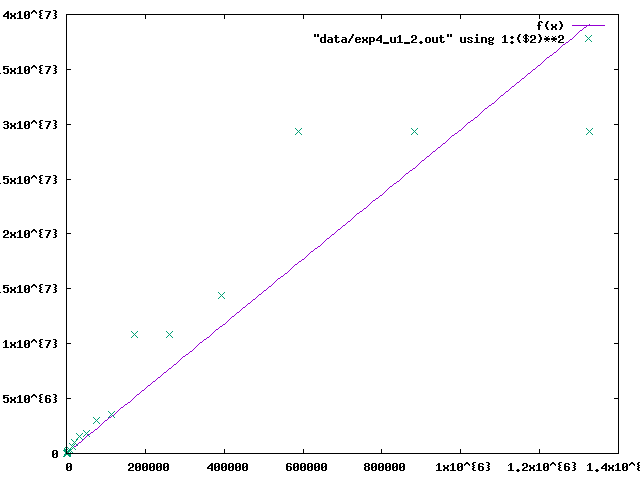
\includegraphics[scale=0.3]{../figs/exp4_u1_2.png}
  \\ $\ulam{1}{2}$\end{tabular} &
\begin{tabular}[c]{@{}c@{}}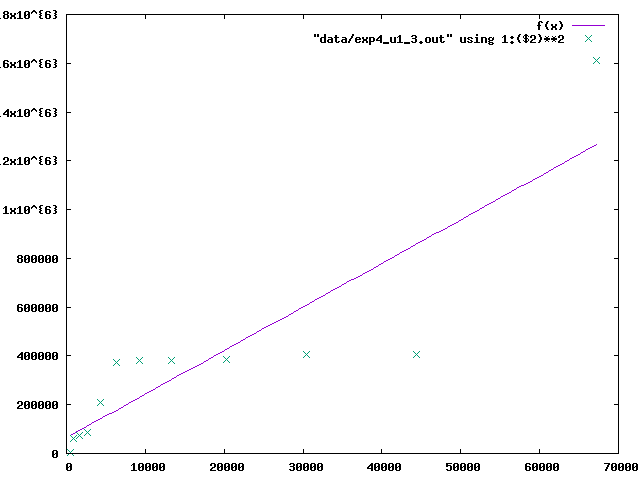
\includegraphics[scale=0.3]{../figs/exp4_u1_3.png}
  \\ $\ulam{1}{3}$\end{tabular} \\\hline
\begin{tabular}[c]{@{}c@{}}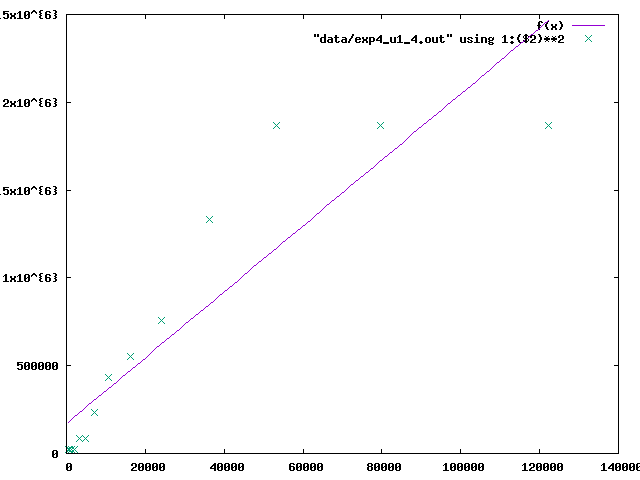
\includegraphics[scale=0.3]{../figs/exp4_u1_4.png}
  \\ $\ulam{1}{4}$\end{tabular} &
\begin{tabular}[c]{@{}c@{}}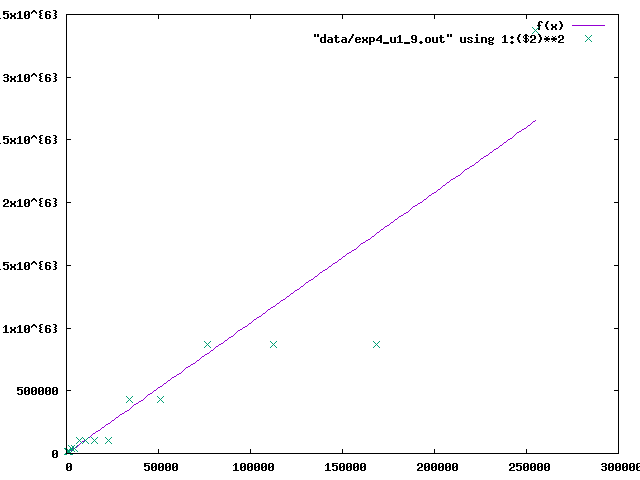
\includegraphics[scale=0.3]{../figs/exp4_u1_9.png}
  \\ $\ulam{1}{9}$\end{tabular} \\\hline
\begin{tabular}[c]{@{}c@{}}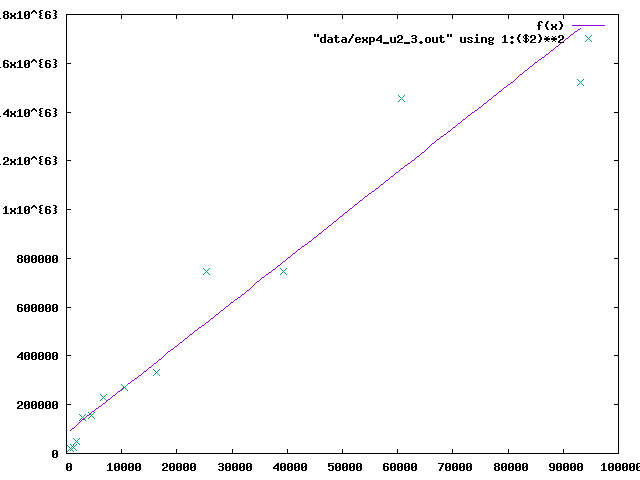
\includegraphics[scale=0.3]{../figs/exp4_u2_3.png}
  \\ $\ulam{2}{3}$\end{tabular} &
\begin{tabular}[c]{@{}c@{}}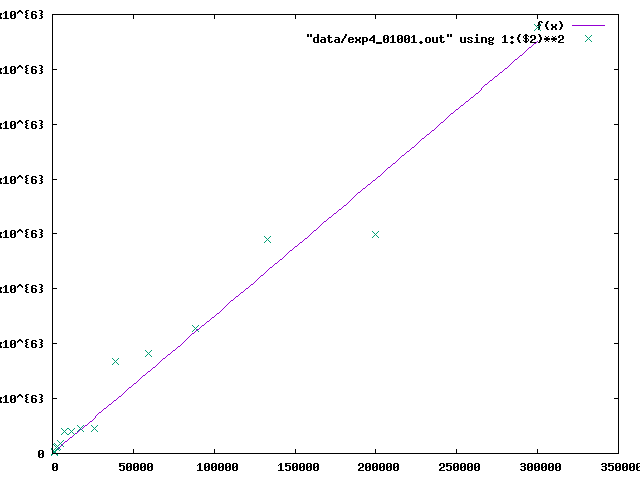
\includegraphics[scale=0.3]{../figs/exp4_01001.png}
  \\ $\theta(01001)$\end{tabular} \\\hline
\begin{tabular}[c]{@{}c@{}}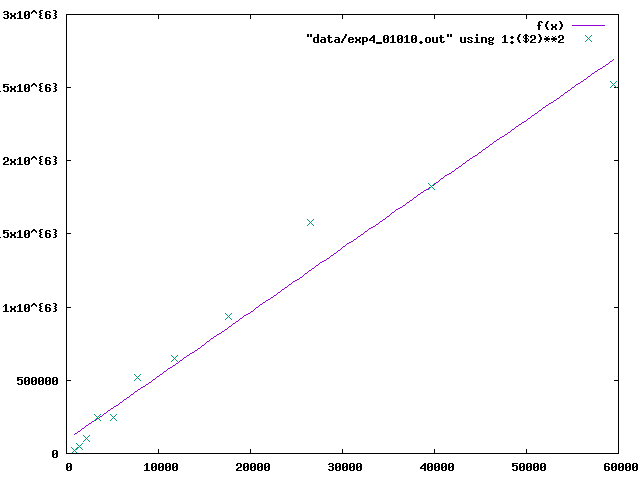
\includegraphics[scale=0.3]{../figs/exp4_01010.png}
  \\ $\theta(01010)$\end{tabular} &
\begin{tabular}[c]{@{}c@{}}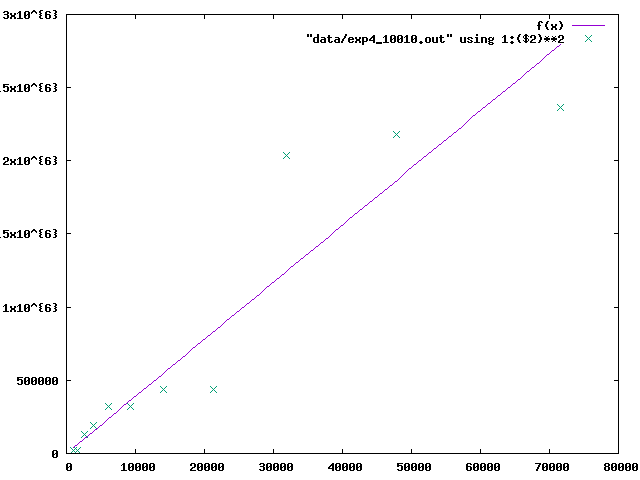
\includegraphics[scale=0.3]{../figs/exp4_10010.png}
  \\ $\theta(10010)$\end{tabular} \\\hline
\end{tabular}
\end{center}
\end{figure}

These suggest, if somewhat loosely, that the $d_N = \Theta(\sqrt{N})$,
(with some oscillation around the line of best fit).  In particular,
there is some $c$ with $d_N \leq c \sqrt{N}$.  

\chapter{Distribution}

As we have remarked before, a sequence $A$ having a large Fourier
coefficient at $\alpha$ suggests $A$ should not be equidistributed
modulo $\lambda = \frac{2\pi}{\alpha}$.  Indeed, we have
experimentally found large Fourier coefficients for many of the
sequences we have considered, and if we take the distribution of these
sequences modulo the corresponding values of $\lambda$, we get
non-uniform, continuous-looking distributions as in figure
\ref{fig:dist_sample}.

\begin{figure}
\caption{Some distribuions of $A$ mod $\lambda_A$}\label{fig:dist_sample}
\begin{center}
\begin{tabular}{cc}
\begin{tabular}[c]{@{}c@{}}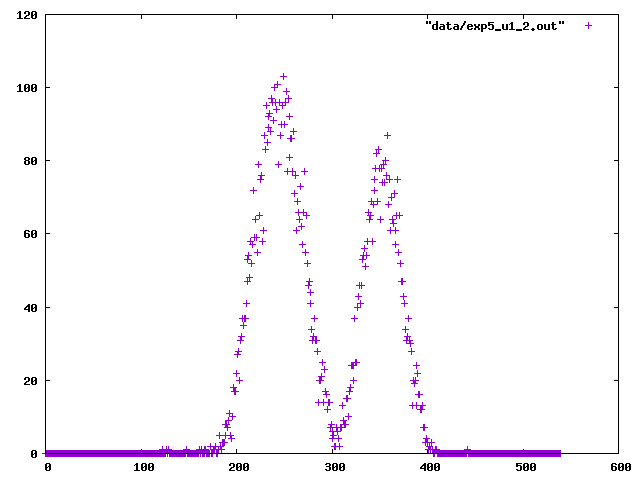
\includegraphics[scale=0.3]{../figs/exp5_u1_2.png}
  \\ $\ulam{1}{2}$\end{tabular} &
\begin{tabular}[c]{@{}c@{}}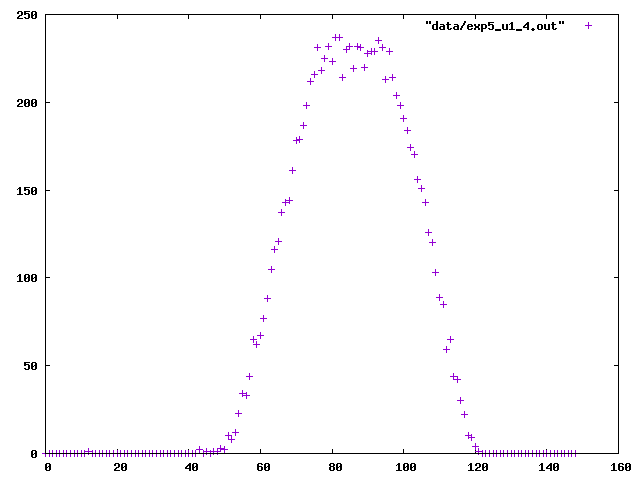
\includegraphics[scale=0.3]{../figs/exp5_u1_4.png}
  \\ $\ulam{1}{3}$\end{tabular} \\\hline
\end{tabular}
\end{center}
\end{figure}

In this section, we will examine how what we have learned about the
spectrum might control various features about the corresponding
distributions.

\section{Distrubution of $r_{A+A}$}

The common feature of the \relevant sets that we have been considering
is that whether $x$ is in one of these sets $A$ is determined by how
many ways we can write $x$ as a sum $x = a+b$ for $a, b \in A$.  To
study this, we make the following definitions:

\begin{definition}For $A \subseteq \N$, define the \textbf{sum
    representation counting function} $r_{A+A}$ by

  \[r_{A+A}(x) = \left|\{(a,b) \in A^2 : a+b = x\}\right|\]

  Also define, the \textbf{modified sum representation counting function}

  \[r^*_{A+A}(x) = \left|\{(a,b) \in A^2 : a+b = x ; a < b\}\right|\]

  Finally, define the \textbf{difference representation counting
    function}

  \[r_{A-A}(x) = \left|\{(a,b) \in A^2 : a-b = x\}\right|\]
\end{definition} 

So $r_{A+A}(x) = 0$ is the necessary condition for $x$ to lie in a
sum-free set $A$, as is $r_{A-A}(x) = 0$, whereas $r^*_{A+A}(x) = 1$
is the condition for being in an Ulam sequence $A$.  Likewise, for $x$
in an Ulam sequence $A$, $r_{A-A}(x)$ is the number of times $x$ is
used as a summand in $A$.  (We note that $r_{A-A}$ may be infinite if
$A$ is infinite, but it will make sense when we truncate $A$.)

But we can write formulae for $r_{A+A}(x)$ and $r_{A-A}(x)$ in terms
of the indicator function of $A$:

\[r_{A+A}(x) = \sum_{0 < y < x} A(y)A(x-y)\]
\[r_{A-A}(x) = \sum_{0 < y} A(y)A(x+y)\]
which are exactly the definition of the convolution $(A \ast A)(x)$
and cross-correlation $(A \star A)(x)$ respectively.

$r^*_{A+A}$ is less clean, but we can write,
$2r^*_{A+A}(x) = r_{A+A}(x) - A(x/2)$.  So if we get bounds on
$r_{A+A}(x)$, we can expect to transfer these to bounds of
$r^*_{A+A}(x)$.  Thus we expect that understanding $r_{A+A}$ will be
sufficient to allow us to understand Ulam sequences as well as
sum-free sets.

So if our assertion is that whether a given $x$ is in $A$ is strongly
affected by the value of $x$ modulo the associated $\lambda_A$, then
we might wonder how $r_{A+A}(x)$ depends on the value of $x$ modulo
$\lambda_A$.  We can do this by taking the various congruence classes
$a$ modulo $\lambda$ and computing the average value of $r_{A+A}(x)$
for $x$ ranging over integers congruent to $a$ modulo $\lambda$.  To
do this in practice, we use a rational approximation to $\lambda$.
Plotting these for the first $10^4$ terms of various sequences we get
the plots in figure \ref{fig:rAA}.

\begin{figure}
\caption{Plots of $r_{A+A}$ modulo $\lambda_A$ for various $A$}\label{fig:rAA}
\begin{center}
\begin{tabular}{cc}
\begin{tabular}[c]{@{}c@{}}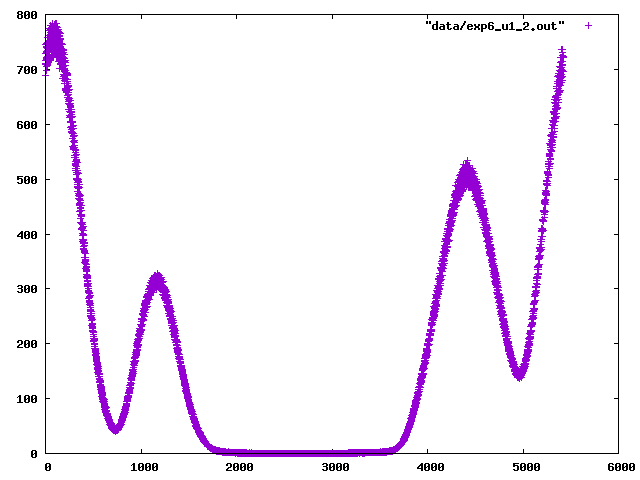
\includegraphics[scale=0.3]{../figs/exp6_u1_2.png}
  \\ $\ulam{1}{2}$\end{tabular} &
\begin{tabular}[c]{@{}c@{}}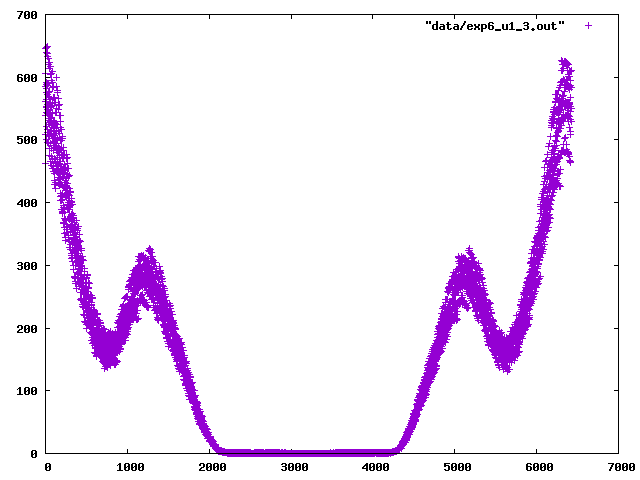
\includegraphics[scale=0.3]{../figs/exp6_u1_3.png}
  \\ $\ulam{1}{3}$\end{tabular} \\\hline
\begin{tabular}[c]{@{}c@{}}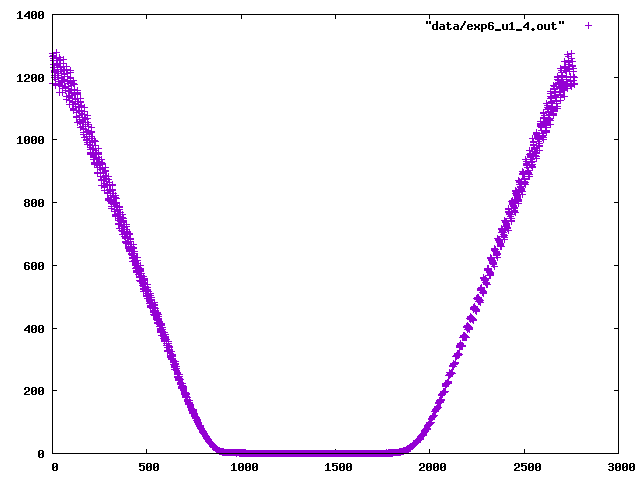
\includegraphics[scale=0.3]{../figs/exp6_u1_4.png}
  \\ $\ulam{1}{4}$\end{tabular} &
\begin{tabular}[c]{@{}c@{}}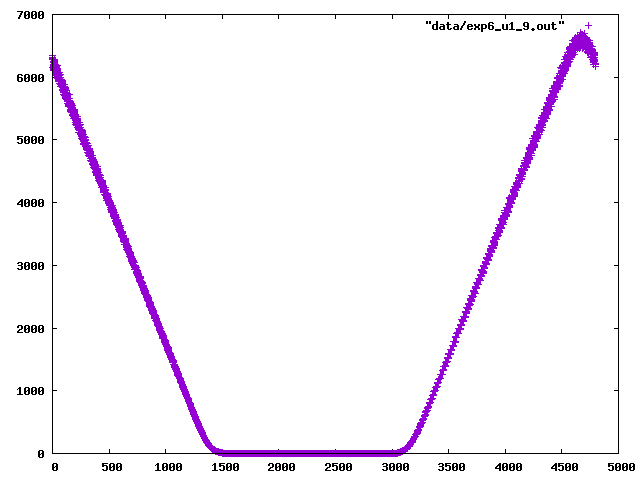
\includegraphics[scale=0.3]{../figs/exp6_u1_9.png}
  \\ $\ulam{1}{9}$\end{tabular} \\\hline
\begin{tabular}[c]{@{}c@{}}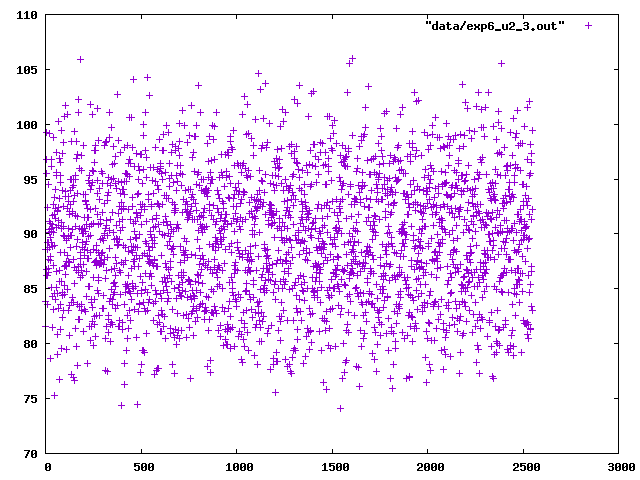
\includegraphics[scale=0.3]{../figs/exp6_u2_3.png}
  \\ $\ulam{2}{3}$\end{tabular} &
\begin{tabular}[c]{@{}c@{}}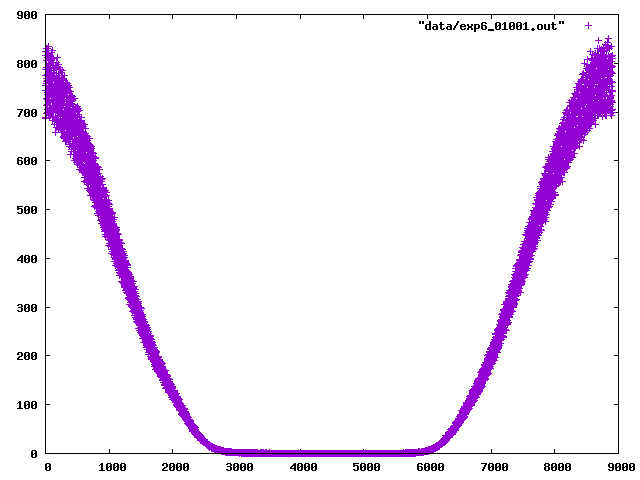
\includegraphics[scale=0.3]{../figs/exp6_01001.png}
  \\ $\theta(01001)$\end{tabular} \\ \hline
\begin{tabular}[c]{@{}c@{}}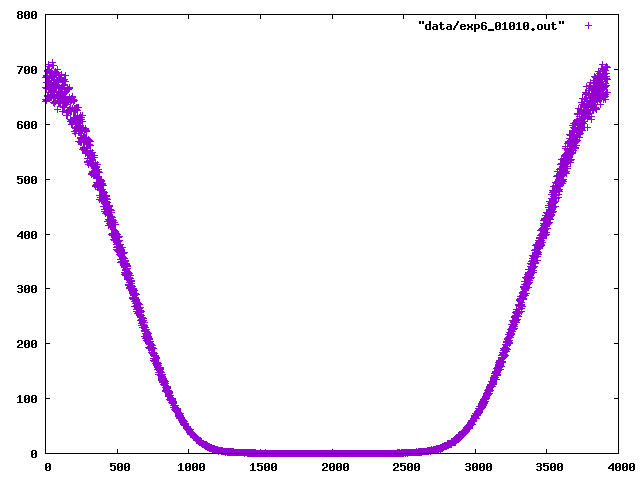
\includegraphics[scale=0.3]{../figs/exp6_01010.png}
  \\ $\theta(01010)$\end{tabular} &
\begin{tabular}[c]{@{}c@{}}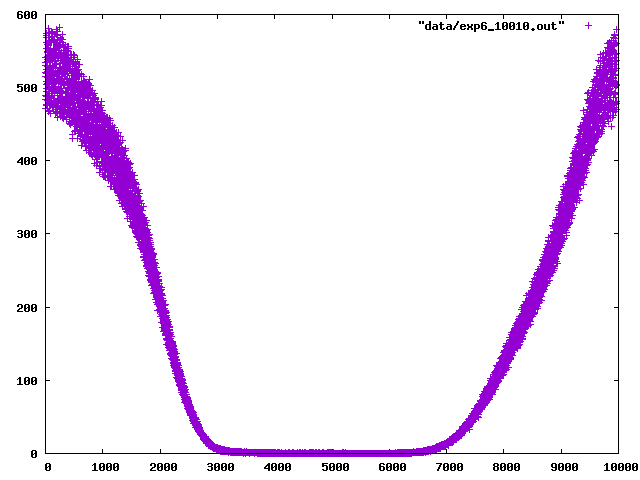
\includegraphics[scale=0.3]{../figs/exp6_10010.png}
  \\ $\theta(10010)$\end{tabular} \\ \hline
\end{tabular}
\end{center}
\end{figure}

The general pattern here seems to be that all these distributions are
large near 0, all close to 0 within the middle third of the interval,
and have some substantial fluctuations in between, from the relatively
extreme example of $\ulam{2}{3}$, to the more sedate examples provided
by the sum-free sets, or by $\ulam{1}{4}$.

These two observations would suggest that near 0, we should not have
any elements of these sequences, and that most of the elements should
lie in the middle third.  Further, for Ulam sequences, this also
suggests that any $x$ that fails to be in the sequence because
$r^*_{A+A}(x) = 0$ should live in the middle third as well, possibly
explaining the gap in the distribution of elements of $\ulam12$ in the
very middle.  

We shall address these observations in the following sections, but we
give a word first about the strategy: The benefit of studying
$r_{A+A}(x)$ is that, being a convolution, we understand its Fourier
transform.  More precisely, truncate $A$ at $N$ and view (as before)
$r_{A_N + A_N}(x)$ and $r_{A_N - A_N}(x)$ as functions on $\Z/2N$.
Then by the convolution theorem (in proposition \ref{prop:fourier}),
we have $(\dft_{2N}r_{A_N + A_N}) = (\dft_{2N}A_N)^2$ and
$(\dft_{2N}r_{A_N - A_N}) = |\dft_{2N}A_N|^2$.  Using Fourier
inversion, then, we can compute $r_{A_N + A_N}$ and $r_{A_N - A_N}$ in
terms of the Fourier coefficients of $A$:

\begin{equation}\label{eqn:rAAsum}r_{A_N + A_N}(x) = 2N \sum_{t=0}^{2N-1} ((\dft_{2N}A)(t))^2 e(\frac{2\pi t}{2N} x)\end{equation}

\begin{equation}\label{eqn:rAAdiff}r_{A_N - A_N}(x) = 2N \sum_{t=0}^{2N-1} |(\dft_{2N}A)(t)|^2 e(\frac{2\pi t}{2N} x)\end{equation}

Since our observations suggest that the spectrum of $A$ is simply
$\alpha\Z$, in particular for $A_N$ we have
$\widehat{A_N}(k\alpha) \leq \frac{C}{k}$ for $k$ up to around
$c\sqrt{N}$ for some constant $c$, and we have lower bounds for
$(\dft_{2N}A)(\alpha)$.  We can then approximate this sum using these
large Fourier coefficients and lump the rest into an error term $R_N$
that we expect (but were unable to prove) is small enough to ignore.
Precisely :


\begin{conjecture}\label{conj:spec_estimate}
  For $A$ a \relevant set with Fourier spectrum $\alpha\Z$, there are
  constants $c, c' > 0$ such that:

\begin{equation}\label{eqn:rAAdiff_err}
  r_{A_N - A_N}(x) = 2N\sum_{|k| < c\sqrt{N}} |(\dft_{2N}A)(k\alpha)|^2 e(k\alpha x) + R_N
\end{equation}

\begin{equation}\label{eqn:rAAsum_err}
  r_{A_N + A_N}(x) = 2N\sum_{|k| < c'\sqrt{N}}(\dft_{2N}A)^2(k \alpha) e(k\alpha x) + R'_N
\end{equation}
  
Where $|R_N|$ and $|R'_N|$ are both $o(N)$ as $N \to \infty$.  
\end{conjecture}

\begin{proof}[Computational evidence]

We compute in \icode{experiment7B} the values of 

\[R'_N = r_{A_N + A_N}(x) - 2N\sum_{|k| < \sqrt{2N}}(\dft_{2N}A)^2(k
  \alpha) e(k\alpha x)\] for various random values of $x$ and each of
our various sequences $A$.  We let $\widetilde{R}_N$ be the maximum
value we see for this quantity over all the $x$ we sample, and put
into table \ref{tab:rAA_est_error}.  Already with the relatively
conservative (relative to observed values of $d_N$) value of
$c' = \sqrt{2}$, we find these to be small relative to $N$, suggesting
that with careful tuning of this parameter we could estimate
$r_{A+A}(x)$ as accurately as needed.

\begin{table}
\caption{Estimation of error in using $\alpha\Z$ to compute
  $r_{A+A}(x)$}\label{tab:rAA_est_error}
\centering
\begin{tabular}{llll}
$A$ & $N$ & $\widetilde{R}_N$ & $\frac{\widetilde{R}_N}{N}$
  \csvreader{datafiles/rAA_est_u1_2.csv}{}
  {\\$\ulam{1}{2}$ & \csvcoli & \csvcolii & \csvcoliii}\\\hline
                                          
  \csvreader{datafiles/rAA_est_u1_3.csv}{}
  {\\$\ulam{1}{3}$ & \csvcoli & \csvcolii & \csvcoliii}\\\hline

  \csvreader{datafiles/rAA_est_u1_4.csv}{}
  {\\$\ulam{1}{4}$ & \csvcoli & \csvcolii & \csvcoliii}\\\hline

  \csvreader{datafiles/rAA_est_u1_9.csv}{}
  {\\$\ulam{1}{9}$ & \csvcoli & \csvcolii & \csvcoliii}\\\hline

  \csvreader{datafiles/rAA_est_u2_3.csv}{}
  {\\$\ulam{2}{3}$ & \csvcoli & \csvcolii & \csvcoliii}\\\hline

  \csvreader{datafiles/rAA_est_01001.csv}{}
  {\\$\theta(01001)$ & \csvcoli & \csvcolii & \csvcoliii}\\\hline

  \csvreader{datafiles/rAA_est_01010.csv}{}
  {\\$\theta(01010)$ & \csvcoli & \csvcolii & \csvcoliii}\\\hline

  \csvreader{datafiles/rAA_est_10010.csv}{}
  {\\$\theta(10010)$ & \csvcoli & \csvcolii & \csvcoliii}\\\hline
\end{tabular}
\end{table}

\end{proof}

This is what we shall attempt to exploit in the following section, but
before then, a word about the actual distributions of $r_{A+A}$ that
we plotted above: 

\begin{proposition}
  Let $A$ be one of our \relevant sets, and let $\frac{m}{k}$ be a
  rational approximation to $\lambda_A$, so $\alpha$ is approximated
  by $\widetilde{\alpha} = \frac{2\pi k}{m}$.  Let $f_N(x)$ be the
  function from $\Z/m \to \R$ that averages the values of
  $r_{A_N+A_N}(t)$ for $t = x \mod{\lambda}$, i.e. $kt = x \mod{m}$.

  That is, 
  \[f_N(x) = \frac{m}{N} \sum_{kt = x\ \!(m), t < N} r_{A+A}(t)\]

  Then we can express: 

  \[f_N(x) = \sum_{l=0}^{m-1} e(\frac{-2\pi x l}{m}) \widehat{A_N}(l\widetilde{\alpha})^2\]
\end{proposition}

\begin{proof}

This follows by the usual trick of expressing the indicator function
of a congruence class mod $m$ using an exponential sum.  In our case: 


\[1(kt = x\!\!\!\!\mod{m}) = \frac{1}{m}\sum_{l=0}^{m-1} e(\frac{2\pi
    (kt-x)}{m}l)\]

So if we simply do this substitution and reverse the order of
summation, we get: 

\begin{eqnarray*}
  f_N(x) &=& \frac{m}{N} \sum_{kt = x\ \!(m), t < N} r_{A+A}(t)\\
         &=& \frac{m}{N} \sum_{t = 0}^{N-1} r_{A+A}(t)1(kt = x\!\!\!\!\mod{m})\\
         &=& \frac{m}{N} \sum_{t = 0}^{N-1}
             r_{A+A}(t)\frac{1}{m}\sum_{l=0}^{m-1} e(\frac{2\pi (kt-x)}{m}l)\\
         &=& \sum_{l=0}^{m-1} \frac{1}{N} \sum_{t = 0}^{N-1}
             r_{A+A}(t) e(\frac{2\pi (kt-x)}{m}l)\\
         &=& \sum_{l=0}^{m-1} e(\frac{-2\pi x l}{m}) \frac{1}{N} \sum_{t = 0}^{N-1}
             r_{A+A}(t) e(\frac{2\pi klt}{m})\\
         &=& \sum_{l=0}^{m-1} e(\frac{-2\pi x l}{m}) \widehat{r_{A+A}}(l\widetilde{\alpha})\\
         &=& \sum_{l=0}^{m-1} e(\frac{-2\pi x l}{m}) \widehat{A_N}(l\widetilde{\alpha})^2\\
\end{eqnarray*}

\end{proof}

Thus if we had more precise knowledge of the argument of
$\widehat{A_N}(\alpha)$ we could perhaps deduce the features we want.
For example, when $x$ is close to zero, this sum would be dominated by
the first two terms and so we should be able to show that it is large.
Or when $x$ is close to $\frac{m}{2}$, this sum should be small since
it will then be an alternating sum.

\section{Distribution mod $\lambda$}

As mentioned, the distributions of various $U(a,b)$ and $\theta(s)$
modulo their respective $\lambda$ values are non-uniform, and seem to
have most (but not all) of their support in the middle third of the
interval $[0,\lambda]$.  For example, if we take the first $10^4$
elements of each sequence and take a rational approximation
$\lambda \approx \frac{m}{k}$ and plot, for each congruence class $r$
mod $m$ how many $a \in A$ have $ka \cong r \mod{m}$, then we get the
plots in figure \ref{fig:dists}

\begin{figure}
\caption{Distributions of various $A$ modulo $\lambda_A$}\label{fig:dists}
\begin{center}
\begin{tabular}{cc}
\begin{tabular}[c]{@{}c@{}}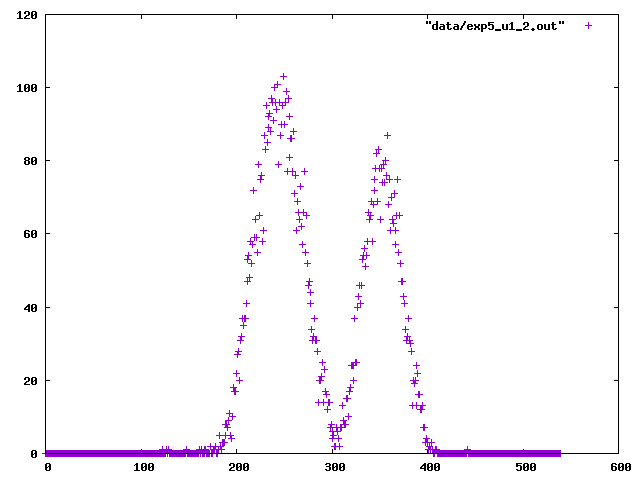
\includegraphics[scale=0.3]{../figs/exp5_u1_2.png}
  \\ $\ulam{1}{2}$\end{tabular} &
\begin{tabular}[c]{@{}c@{}}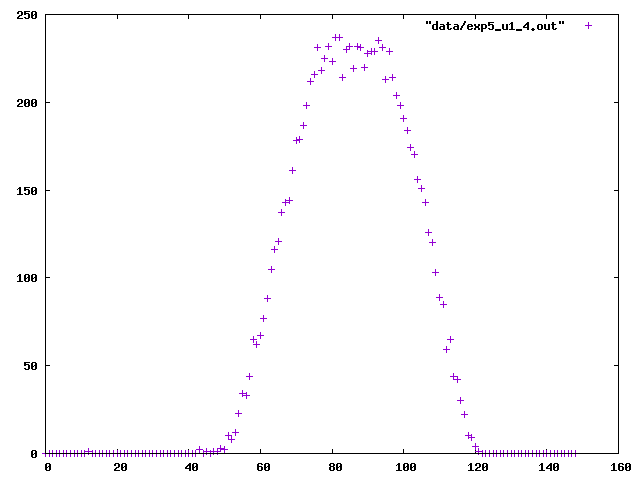
\includegraphics[scale=0.3]{../figs/exp5_u1_4.png}
  \\ $\ulam{1}{3}$\end{tabular} \\\hline
\begin{tabular}[c]{@{}c@{}}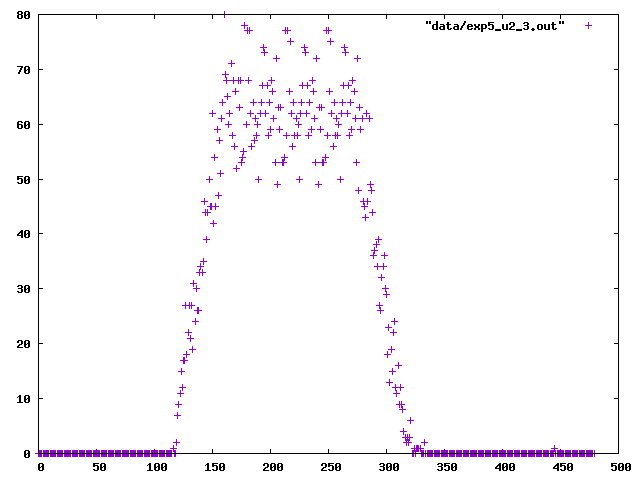
\includegraphics[scale=0.3]{../figs/exp5_u2_3.png}
  \\ $\ulam{1}{4}$\end{tabular} &
\begin{tabular}[c]{@{}c@{}}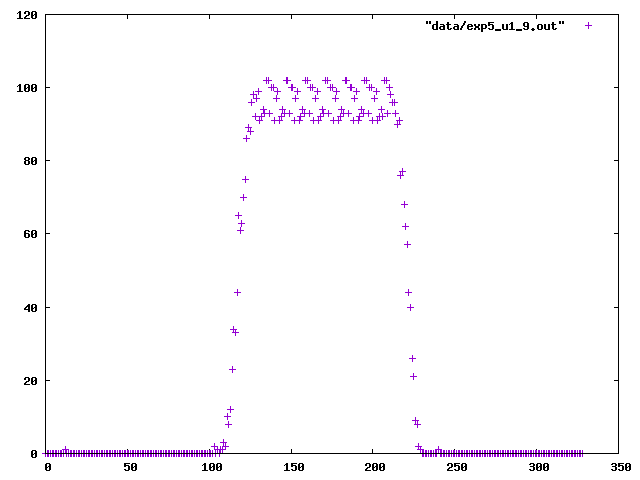
\includegraphics[scale=0.3]{../figs/exp5_u1_9.png}
  \\ $\ulam{1}{9}$\end{tabular} \\\hline
\begin{tabular}[c]{@{}c@{}}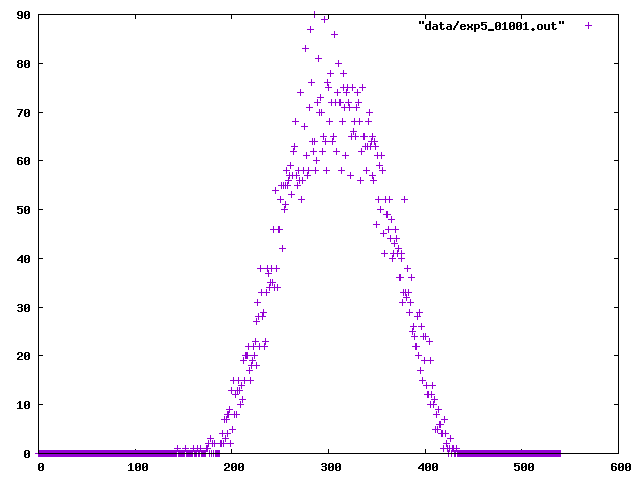
\includegraphics[scale=0.3]{../figs/exp5_01001.png}
  \\ $\theta(01010)$\end{tabular} &
\begin{tabular}[c]{@{}c@{}}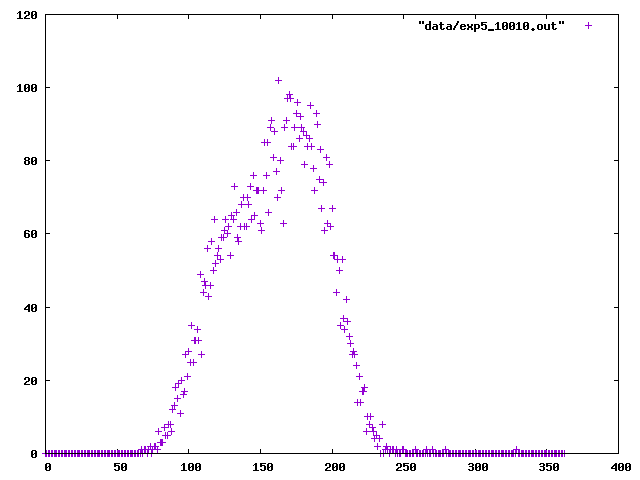
\includegraphics[scale=0.3]{../figs/exp5_10010.png}
  \\ $\theta(10010)$\end{tabular} \\ \hline
\end{tabular}
\end{center}
\end{figure}

There are many observations to be made, among which:

\begin{enumerate}
\item There seem to be few elements of each $A$ in some interval
  around 0 modulo $\lambda$.
\item The support of these distributions seems to usually contain the
  middle third modulo $\lambda$.  
\item The distribution of $\ulam{1}{n}$ seems like it might be
  converging to a multiple of the characteristic function of the
  middle third modulo $\lambda$.  
\end{enumerate}

Of these, we will examine in this section the first two.

As a useful piece of notation for expressing the idea of intervals
such as ``the middle third modulo $\lambda$'', we will define as is
standard:

\begin{definition}
For $x \in \R$, define $\normrz{x}$ to be the minimal distance between
$x$ and an integer: $\normrz{x} = \min_{n \in \Z} |x-n|$.
\end{definition}

Thus $\normrz{x} \leq \frac12$ always, and $x$ is in the ``middle
third'', i.e $\left(\frac{\lambda}{3}, \frac{2\lambda}{3}\right)$ mod
$\lambda$ precisely if $\normrz{x/\lambda} > \frac13$.  Likewise, an
interval, (say of radius $\eta$) around zero (mod $\lambda$) is
expressed by the condition $\normrz{x/\lambda} < \eta$.

\subsection{No elements close to 0 mod $\lambda$}

As promised, we move first to investigate why it appears that there
are no elements of $A$ close to integer multiples of $\lambda$.  The
distributions of $r_{A+A}$ would suggest that the reason is that $x$
that are close to $\lambda\Z$ have $r_{A+A}(x)$ large.

As we saw in equation \ref{eqn:rAAsum}, we can express this in terms
of the spectrum of $A$, and hopefully can therefore extract some
information.  In particular, if $\normrz{x/\lambda} < \eta$, then for
$\frac{m}{2N} \approx \lambda$, $e(\frac{2\pi k}{2N} x)$ will be on
the arc between $e(-\eta)$ and $e(\eta)$, making it very close to 1.
So, particularly if we use the approximation given in equation
\ref{eqn:rAAsum_err}, we get: 

\begin{eqnarray*}
  r_{A_N + A_N}(x) &=& 2N \sum_{|k| < c\sqrt{N}}
                       (\dft_{2N}A)(k\alpha)^2 e(k\alpha x) + R_N\\
                   &\approx& 2N \left(\frac{\delta^2}{2} +
                             2\Re((\dft_{2N}A)(\alpha)^2 e(\eta)) + \sum_{k > 1}
                             2\Re((\dft_{2N}A)(k\alpha)^2 e(k\eta))\right) + R_N\\
\end{eqnarray*}

And so if the argument of $(\dft_{2N}A)(\alpha)$ is close to $\pi$ and
if $\eta$ is small enough, then hopefully the term we've pulled out of
the sum dominates this expression and we get that
$r_{A_N + A_N}(x) = O(N)$.  But this requires very precise control
over the argument of $(\dft_{2N}A)(k\alpha)$ that we do not currently
have.

However, at least for truly sum-free sets, we can still pull out a
theorem (as always, conditional on various conjectures about the
spectrum) of this kind by using the fact that for a sum-free set, an
element can be in the set $A$ only if $r_{A-A}(x) = 0$ also.  And,
recalling equations \ref{eqn:rAAsum} and \ref{eqn:rAAsum_err}, this we
can compute using only the magnitudes of the Fourier coefficients,
allowing us to ignore the argument issue completely:

\begin{theorem}\label{thm:hole1}
  Let $A$ be an \relevant set of positive integers with
  $|A_N| = \delta N$.  Suppose that $A$ has spectrum $\alpha\Z$, that
  it satisfes conjecture \ref{conj:decay}, and that the error in
  equation \ref{eqn:rAAsum_err} in fact satisfies $R_N = o(N)$
  (conjecture \ref{conj:spec_estimate}).  Then for some $\eta > 0$,
  $\norm{x/\lambda} < \eta$ implies $r_{A_N-A_N}(x) = \Omega(N)$.
\end{theorem}

\begin{proof}
  Take $x$ with $\normrz{x/\lambda} < \eta$ for $\eta$ to be chosen
  later.  Viewing $A_N$ as usual inside $\Z/2N$, we have
  $x \in A_N - A_N$ viewed inside $\Z/2N$ iff $x \in A_N - A_N$ in
  $\Z$.  So we can use equation \ref{eqn:rAAsum_err}.  In preparation
  for doing this, let $|\widehat{A_N}(\alpha)| = \rho$ (we know
  $\rho > \frac{\delta^2}{2} - O(1/N)$ by \ref{thm:alpha_finitary}),
  and let $k_0$ be such that
  \[\delta^2 + \rho^2 - 4 C^2 \sum_{k=k_0}^\infty \frac{1}{k^2} > 0\]
  (which we know is possible since $\delta > 0, \rho > 0$, and since
  the the sum converges, and so approaches 0 as $k_0 \to \infty$).
  Then if we choose $\eta$ to guarantee that
  $\normrz{k_0 x/\lambda} < \frac14$ (so that $\Re(e(k\alpha x)) > 0$
  for all $k < k_0$), then as $N$ gets large, we have:

  \begin{eqnarray*}
    r_{A_N - A_N}(x) &=& 2N \sum_{|k| < c\sqrt{N}}
                       (\dft_{2N}A)(k\alpha)^2 e(k\alpha x) + R_N\\
                     &\geq& N \delta^2 + 2N
                            |\widehat{A_N}(\alpha)|^2
                            \Re(e_N(\alpha x)) - 2N \sum_{|k| \geq k_0}
                            |\widehat{A_N}(k\alpha)|^2 - |R_N|
  \end{eqnarray*}
  where here, we are using that
  $\Re(|\widehat{A_N}(k\alpha)|^2 e(k\alpha x)) \geq 0$ for
  $1 < k < k_0$ by choice of $\eta$, and that
  $\Re(|\widehat{A_N}(k\alpha)|^2 e(k\alpha x)) \geq
  -|\widehat{A_N}(k\alpha)|^2$ for $k \geq k_0$.  So: 

  \begin{eqnarray*}
    r_{A_N - A_N}(x) &\geq& \frac{\delta^2}{2} N + \frac{\rho^2}{2} N
                            - 2N \sum_{|k| \geq k_0}
                            |\widehat{A_N}(k\alpha)|^2 - |R_N|\\
                     &\geq& \frac{\delta^2}{2} N + \frac{\rho^2}{2} N
                            - 2C^2 N \sum_{|k| \geq k_0}
                            \frac{1}{k^2} - |R_N|\\
  \end{eqnarray*}

  Using \ref{conj:decay} to conclude
  $|\widehat{A_N}(k\alpha)| \leq \frac{C}{k}$ for some constant $C$.
  Thus:

  \[r_{A_N - A_N}(x) \geq \frac{N}{2}\left(\delta^2 + \rho^2 - 4C^2
      \sum_{|k| \geq k_0} \frac{1}{k^2} - \frac{2|R_N|}{N}\right)\]
  which we know by choice of $k_0$ that for $N$ large enough (so that
  conjecture \ref{conj:spec_estimate} can kick in to allow us to
  ignore the $R_N$ term) the value in parentheses is positive, and so
  the whole expression is $\Omega(N)$, as desired.
\end{proof}

For sum-free $A$, this automatically guarantees that no integer within
this interval can be in $A$, as for sum-free sets, $r_{A_N-A_N}(x) >
0$ for any $N$ already implies $x \notin A$: 

\begin{corollary}
If $A$ is a sum-free set satisfying all the conditions of the theorem,
then there is an $\eta > 0$ such that $\normrz{x/\lambda_A} < \eta
\implies x \notin A$.  
\end{corollary}

We can make an analogous statement for Ulam sequences, noting that if
$x$ is in an Ulam sequence $A$ and $r_{A_N - A_N}(x)$ is also large,
then this means that $x$ is a summand for many elements of $A$: 

\begin{corollary}If $A$ is an Ulam sequence, then there is an
  $\eta > 0$ such that $\normrz{x/\lambda_A} < \eta$ implies that $x$
  appears as a summand for elements of $A_N$ some $\Omega(N)$ times.
\end{corollary}

We will see examples of this observation in section 7.

% Also, one will note that the bound we used on the tail sum in the
% above proof was very crude--simply the triangle inequality.  In fact,
% as $N$ gets large this approaches something like

% \[N \int_{\frac{k_0}{N}}^{2\pi} \frac{e^{it}}{t^2}dt\]

% Which is related to standard exponential integrals.  So we can use
% facts about such integrals to bound this particular one analytically
% in terms of $k_0$ and $N$ and get a better result.


% And so if $\widehat{1_A}(k)$ is much larger than all the other Fourier
% coefficients, then we might be able to guarantee that this is
% positive.  For example: If we know that the only Fourier coefficients
% that are nonzero (in the large $N$ limit) are $k\alpha$, then we can
% write this as: 

% \begin{eqnarray*}
% r_{A+A}(x) &\geq& |A|/N + \Re(\widehat{1_A}(\alpha)^2) + \sum_{t > 1}
%  \Re(\widehat{1_A}(t \alpha)^2 e(tx))\\
%  &\geq& |A|/N + \Re(\widehat{1_A}(\alpha)^2) - \sum_{t > 1}
%  |\widehat{1_A}(t \alpha)|^2\\
% \end{eqnarray*}

% So if $|\widehat{1_A}(\alpha)|$ is large enough--say, $c$, and
% $|\widehat{1_A}(t \alpha)|$ decays appropriately as $t$ grows--say is
% less than $\frac{A}{t}$, then we get:

% % See, for example,
% % http://www-m7.ma.tum.de/foswiki/pub/M7/Analysis/Fourier13/lecture9.pdf


% \begin{eqnarray*}
% r_{A+A}(x) &\geq& |A|/N + c^2 - \sum_{t > 1}\frac{A^2}{t^2}\\
% &=& \delta + c^2 - A^2\left(\frac{\pi^2}{6}-1\right)\\
% &\geq& \delta + c^2 - 0.644 A^2\\
% \end{eqnarray*}

% So depending on the precise constants involved, we might end up with a
% conclusion that every such $x$ that lands close to 0 mod $\lambda$
% necessarily has many representations and is therefore disqualified
% from being an Ulam number for that reason.  

% \subsection{Few Ulam numbers outside middle third mod $\lambda$}

% A conjecture of Gibbs states...

\subsection{Numbers that are not sums of Ulam numbers close to middle mod $\lambda$}

Another behaviour suggested by the distribution of $r_{A+A}$ concerns
non-Ulam numbers, and specifically numbers $x$ that fail to be Ulam
because $r^*_{A+A}(x) = 0$.  The fact that it appears
$r_{A+A}(x) > 0$ outside the middle third suggests that all of these
would lie within the middle third.

Indeed, if we take such numbers and plot their distribution mod
$\lambda$, as we do in \icode{experiment10}, we get figure
\ref{fig:nonsums}.

\begin{figure}
\caption{Numbers not in $A$ nor in $A+A$ plotted modulo $\lambda_A$}\label{fig:nonsums}
\begin{center}
\begin{tabular}{cc}
\begin{tabular}[c]{@{}c@{}}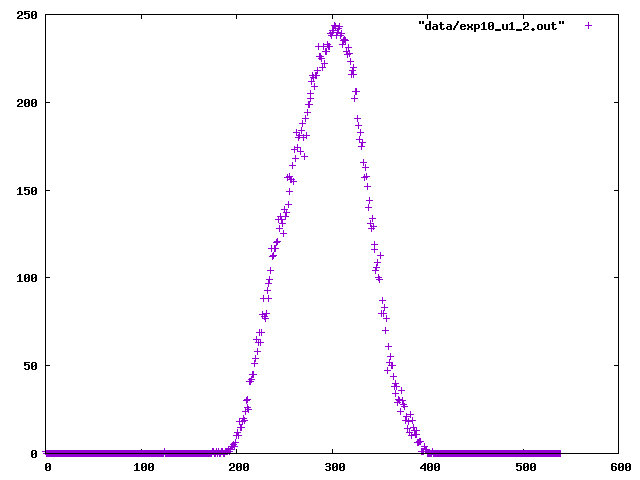
\includegraphics[scale=0.3]{../figs/exp10_u1_2.png}
  \\ $\ulam{1}{2}$\end{tabular} &
\begin{tabular}[c]{@{}c@{}}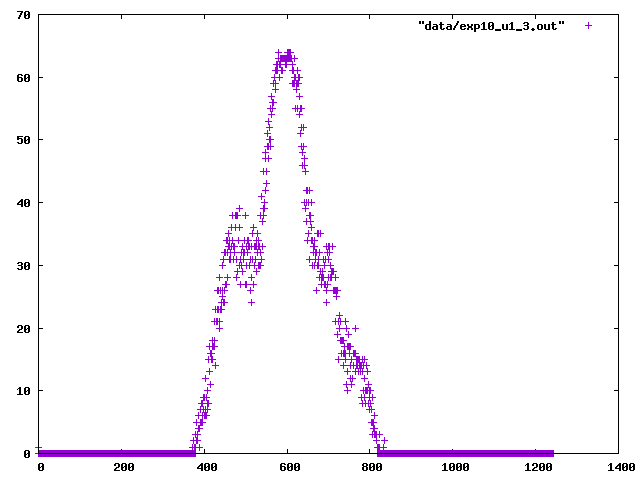
\includegraphics[scale=0.3]{../figs/exp10_u1_3.png}
  \\ $\ulam{1}{3}$\end{tabular} \\\hline
\begin{tabular}[c]{@{}c@{}}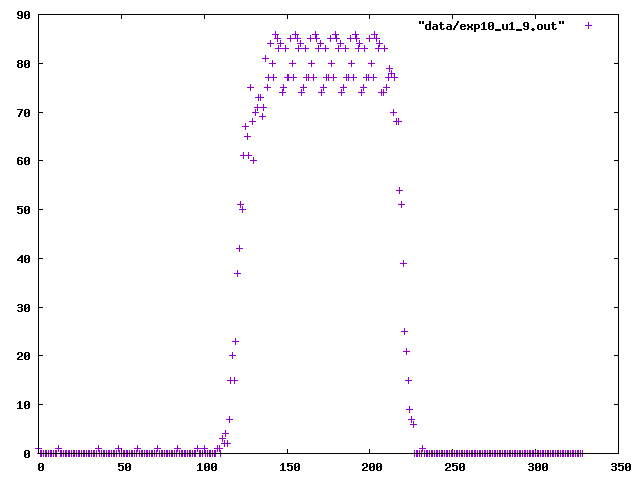
\includegraphics[scale=0.3]{../figs/exp10_u1_9.png}
  \\ $\ulam{1}{9}$\end{tabular} &
\begin{tabular}[c]{@{}c@{}}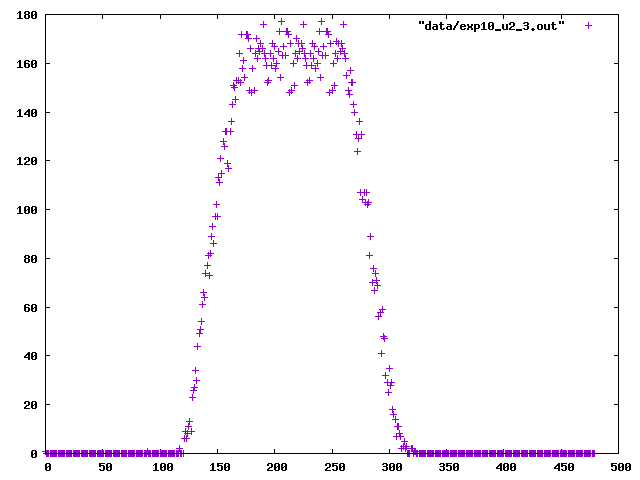
\includegraphics[scale=0.3]{../figs/exp10_u2_3.png}
  \\ $\ulam{2}{3}$\end{tabular} \\
\end{tabular}
\end{center}
\end{figure}

These plots share many features with the distributions of the Ulam
numbers modulo $\lambda$, bolstering the idea that it isn't the
feature of ``being an Ulam number'' as such that creates the
distribution, but simply the relationship between $r_{A+A}(x)$ and
being in $A$.  Specifically, for Ulam sequences $A$, $x$ being in $A$
is related to $r_{A+A}(x)$ is small, whether it is 2 or 3 and so
$x \in A$ or it is literally 0, and $x$ is in the sets we're
considering in this section, such $x$'s still show the same bias
modulo $\lambda$,

We end with a final remark that within the first $10^4$ elements of
each of these Ulam sequences, we have many elements that fail to
qualify by having no representations, as enumerated in table
\ref{tab:nonsums_count}.  

\begin{table}
\caption{Count of non-sums in $A_N$ up to
  $N$}\label{tab:nonsums_count}
\centering
\begin{tabular}{lll}
$A$ & $N$ (with $|A_N| = 10^4$) & $|\{x < N : r^*_{A+A}(x) = 0\}|$\\
$\ulam{1}{2}$ & 132788 & 24415\\
$\ulam{1}{3}$ & 78819 & 13445\\
$\ulam{1}{9}$ & 58114 & 7859\\
$\ulam{2}{3}$ & 108466 & 23052
\end{tabular}
\end{table}

\section{Non-uniformity/Regularity}

% \begin{definition}$A \subseteq \N$ is
%   \textbf{$\epsilon, \beta$-regular} if there is a subset
%   $S \subseteq \R/\Z$ such that
%   $\abr{A^c, \pi_\beta\inv(S)} < \epsilon$, where $\pi_\beta$ is the
%   composition $\Z \to \beta\Z \to \R/\Z$, the first map being
%   multiplication by $\beta$ and the second being reduction modulo
%   $\Z$.
% \end{definition}

Without any unconditional result describing the distributions of our
various $A$ modulo $\lambda_A$, we might ask whether we can at least
guarantee some kind of non-uniformity of these distributions.  For
example, can we find a set $E \subseteq \R/\Z$ such that if
$\pi : Z \to \R/\Z$ is $x \mapsto x/\lambda \mod{1}$, then
$|A_N \cap \pi\inv(E)|/N$ is creater than what might be expected from
the sizes of these sets alone, namely
$\frac{|A_N|}{N}\frac{|\pi\inv(E)_N|}{N}$?  In fact, we can do
slightly better:

\begin{theorem}\label{thm:regularity}
  For $A$ an \relevant set, and let $\alpha$ be the maximal Fourier
  coefficient, and define
  $E_{t} = \{n \in [N] : \Re(e(\alpha n)) \leq \eta\}$ (roughly, the
  set of integers that land in an interval of radius $\eta$ centred at
  $\lambda/2$ modulo $\lambda$.  Then there is a $\eta$ such that
  $\abr{A_N, E_{\eta,N}} = |A_N \cap E_{\eta,N}| \geq \delta^2/4 +
  \delta \frac{|E_{\eta,N}|}{N}$.
\end{theorem}

\begin{proof}
  Let $f(t) = A(t) - \delta$ be the ``balanced'' indicator function of
  $A$.  Then we know from \ref{thm:alpha_real} that $\frac{1}{N}\sum_{t=0}^{N-1}
  f(t)\Re(e(\alpha t)) \leq -\frac{\delta^2}{2}$.  The key here is to
  write: 

  \[\Re(e(\alpha t)) = 1-\int_{-1}^1 E_\eta(t)d\eta\]

  Then 
  \begin{eqnarray*}
    \frac{\delta^2}{2} &\leq& -\frac{1}{N}\sum_{t=0}^{N-1}
                              f(t)\Re(e(\alpha t)) \\
                       &=& -\frac{1}{N}\sum_{t=0}^{N-1}
                           f(t) +  \frac{1}{N}\sum_{t=0}^{N-1}
                           \int_{-1}^1 f(t) E_\eta(t)d\eta\\
                       &=& \frac{1}{N}\sum_{t=0}^{N-1}
                           \int_{-1}^1 f(t) E_\eta(t)d\eta\\
                       &=& \int_{-1}^1 \abr{f, E_\eta} d\eta
\end{eqnarray*}

Thus $\abr{f, E_\eta} \geq \frac{\delta^2}{4}$ for some $\eta$.  But
$f = A - \delta$, so 
\[\abr{A, E_\eta} \geq \frac{\delta^2}{4} + \abr{\delta, E_\eta} =
  \frac{\delta^2}{4} + \delta \frac{|E_{\eta,N}|}{N}\]
And this is what we wanted to show.
\end{proof}

So this is our first basic result in the direction we want to go,
namely towards some statement that large \relevant sets are \relevant
for local reasons.  Another simpler example of this comes from
thinking about regular such sequences:

\begin{theorem}\label{thm:regular_sumfree}
  If $A$ is a regular 1-additive or sum-free set, then there is an
  $N > 0$, an $m$, and a sum-free $E \subseteq \Z/m$ such that if
  $\pi : \Z \to \Z/m$ is the quotient map, then $A$ and $E$ agree for
  all integers larger than $N$.  In other words, such $A$ eventually
  agree with a locally sum-free set. 
\end{theorem}

\begin{proof}
  If $A$ is regular, then there is an $N > 0$ and a modulus $m$ with a
  list of congruence classes $a_1, \ldots, a_n$ mod $m$ such that for
  all $x > N$, $x \in A$ if and only if $x = a_i \mod{m}$ for some
  $i$.  

  If $E = \{a_1, \ldots, a_n\} \subseteq \Z/m$ is not sum-free, then there
  are $i, j, k$ with $a_i + a_j = a_k \mod{m}$.  Supposing, as we may
  without loss, that $0 \leq a_r < m$ for all $r$, then
  $a_i + a_j = a_k + m\epsilon$ for $\epsilon = 0$ or $\epsilon = 1$.

  Now, define five numbers $x, y, z, w, c$ by $x = Nm + a_i$,
  $y = Nm + a_j$, $z = (N+1)m + a_i$, $w = (N+1)m+a_j$, and
  $c = (2N+2+\epsilon)m + a_k$.  These are all distinct, since
  $0 \leq a_i, a_j, a_k < m$.  They are also all in $A$, since they
  are in $E$ modulo $m$, and are all greater than $N$.  However,
  $x+w = c$ and $y+z = c$.  So, $c$, an element of $A$, has two
  distinct representations as sums of distinct smaller elements of
  $A$, contradicting the 1-additivity of $A$.

  Thus $E$ had to have been sum-free, and then we have that for
  $x > N$, $x \in A \iff x \in \pi\inv(E)$, where $\pi : \Z \to \Z/m$
  is the quotient map and $E \subseteq \Z/m$ is sum-free, as desired.
\end{proof}

\chapter{Structure of $\ulam{1}{2}$}

We now turn specifically to $A = \ulam{1}{2}$, the original sequence
of Ulam numbers.  Much of the analysis in this section could be ported
to other Ulam sequences, but we do not do so here.

\section{Distribution of summands}

We know that each element $a_n \in A$ is a sum $a_i + a_j$ of smaller elements
with $a_i < a_j$.  This gives us much structure to play with: 
\begin{itemize}
\item For example, for each $x \in A$, let
  $S_x = \{y \in A : x + y \in A\}$.  We might wonder about the sizes
  of $S_x$ for various $x$--is it roughly constant among all $x$, or
  are there very few $x$ that act as summands for elements of $A$?
\item If we write each $a_n = a_i + a_j$ where $i < j$, what is the
  distribution of the values of $i$ that show up?  (That is, what is
  the distribution of small summands?)  What about the values of
  $j$?  Perhaps more reasonable would be to ask about the distribution
  of $n-j$ (so a question about the distribution of large summands).
\item If we start by breaking up an $a \in A$ as $a = x+y$ for $x < y$
  both in $A$, we can then break up $x$ and $y$ themselves into sums
  of Ulam numbers, and repeat until we get down to writing $a$ as a
  sum of 1s and 2s.  So we can wonder about the proportion of 1s and
  2s in this factorisation.  
\end{itemize}

\subsection{Distribution of large summands}
We note first that if 2 or 3 is the small summand of $a_{n+1}$, and if
$a_n > 6$, then the large summand is necesarily $a_n$ (if 2 is the
small summand and $a_n$ is not the large summand, then $a_{n+1}$ would
be $a_n + 1$ which is impossible since this would mean
$a_n + a_1 = a_{n-1} + a_2$, which violates 1-additivity.  If 3 is the
small summand and $a_n$ is not the large summand, then
$a_{n+1} = a_{n-1} + 3$ or $a_{n+1} = a_{n-2} + 3$, either way giving
$a_{n+1} = a_n + 1$ or $a_{n+1} = a_n + 2$, either of which would give
an honestly distinct (since $a_n > 6$) second way of representing
$a_{n+1}$ as a sum of smaller Ulam numbers, again violating
1-additivity.)

This means that as often as 2 or 3 is the small summand, (which we
will see is a large proportion of the time), the large summand will be
the last thing in the list so far.  When looking at the large summand,
then, it seems like it may be interesting to consider how many indices
from the end it lives, rather than its actual value.  That is, for
small summand $a_i$, we should consider for what values of $j$ is
$a_n = a_i + a_{n-j}$.  We compute these in \icode{experiment13}.
Some post-processing of the output gives us table
\ref{tab:large_summands}, which accounts for over 9000 of the $a_n$
for $n \leq 10^4$.

\begin{table}
\caption{Large summands}\label{tab:large_summands}
\centering
\small
\begin{tabular}{llll}
  $|n : a_i + a_{n-j} = a_n|$ & $a_i$ & $i$ & $n-j$
  \csvreader{datafiles/large_summands.csv}{}
  {\\\csvcoli & \csvcolii & \csvcoliii & \csvcoliv}
\end{tabular}
\end{table}

All told there are 312 different pairs $(i, n-j)$ that appear in the
first $10^4$ Ulam numbers, including only $69$ distinct values of $i$
and 159 values distinct values of $n-j$.  

Note in particular that there being only 312 distinct such pairs means
that technically, to compute the first 10000 Ulam numbers, we would
only have to check 312 possibilities for each, if we somehow knew
which possibilities to check ahead of time.

\subsection{Distribution of small summands}

We note with interest the observation of Steinerberger
\cite{steinerberger:preprint} that $\cos(\alpha a_i) < 0$ for all
$a_i$ other than 2, 3, 47, and 69.  In particular, these were also the
$a_i$ that showed up most frequently as summands in our earlier
computation.  We also note that $\cos(\alpha a_i) < 0$ is just the
condition that $\normrz{x/\lambda} < \frac14$.

So we compute which how often each $a$ appears as the smaller summand
of a later $a_i$ (that is, we compute $|S_a|$) and we compute
$\normrz{a/\lambda}$ for each and sort by this quantity.  We note what
looks like a very strong correlation between how often $a$ shows up as
a summand and $\normrz{a/\lambda}$ in the resulting table
\ref{tab:small_summands}, computed by \icode{experiment12}.

\begin{table}
\caption{Small summands}\label{tab:small_summands}
\centering
\begin{tabular}{lll}
  $a$ (with $|S_a| > 10$) & $|S_a|$ & $\normrz{a/\lambda}$
  \csvreader{datafiles/small_summands.csv}{}
  {\\\csvcoli & \csvcolii & \csvcoliii}
\end{tabular}
\end{table}

\subsection{Distribution of complements}
In the cases Steinerberger looks at, the resulting non-uniform
distributions consist usually of multiple peaks.  In the case of
$\ulam{1}{2}$, one of these peaks looks a little misshapen, so we
might reasonably wonder what each of these peaks actually is.

To get a handle on this, we take the Ulam sequence mod 5422, and
multiply it by 2219 ($5422/2219$ being a good rational approximation
to $\lambda$).  Of course, this gives rise to the usual
distribution we've come to expect in figure \ref{fig:dist_ulam12}

\begin{figure}
\caption{Distribution of $\ulam12$ modulo
  $\lambda$}\label{fig:dist_ulam12}
\centering
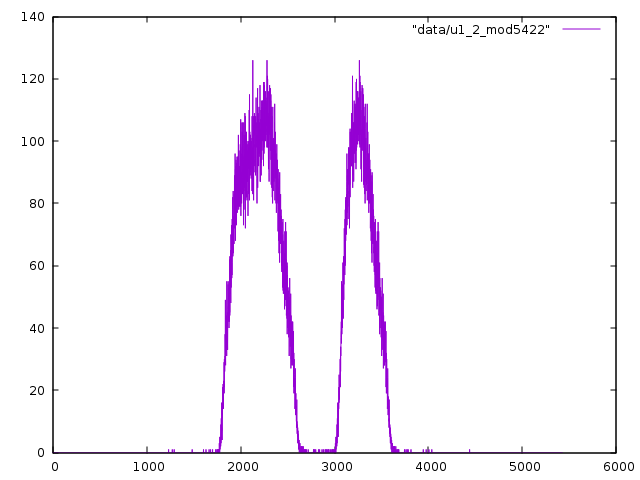
\includegraphics[scale=0.5]{../figs/u1_2_mod5422.png}
\end{figure}

Supposing we look instead only at $a_n$'s for which 2, say is a
summand--that is, the distribution of $S_2$.  Then we get the nice
picture in figure \ref{fig:summands2}, and likewise for $S_{47}$, say,
in figure \ref{fig:summands47}.

\begin{figure}
\caption{Distribution of $S_2$}\label{fig:summands2}
\centering
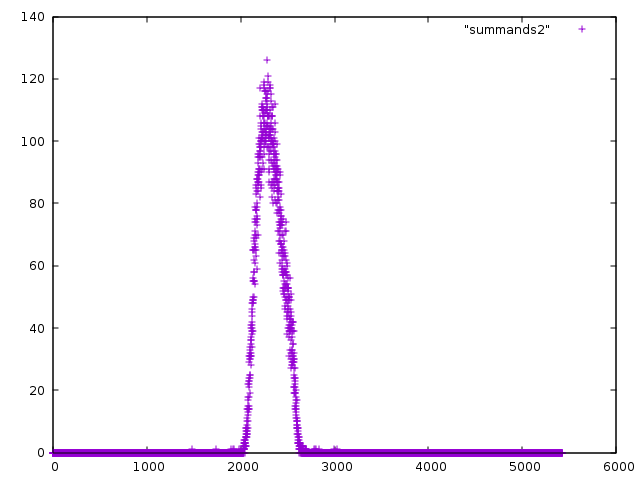
\includegraphics[scale=0.5]{../figs/summands2.png}
\end{figure}

\begin{figure}
\caption{Distribution of $S_{47}$}\label{fig:summands47}
\centering
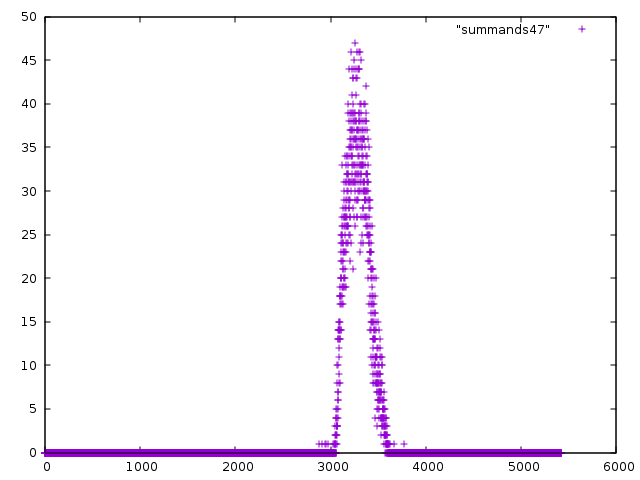
\includegraphics[scale=0.5]{../figs/summands47.png}
\end{figure}

These are relatively clean-looking distributions, by comparison.  If
we plot these graphs for all of the top 25 most common summands all in
one picture, we notice that these seem to be the components of the two
observed peaks, illustrated in figure \ref{fig:summands}.

\begin{figure}
\caption{Distribution of all $S_a$ for small summands $a$}\label{fig:summands}
\centering
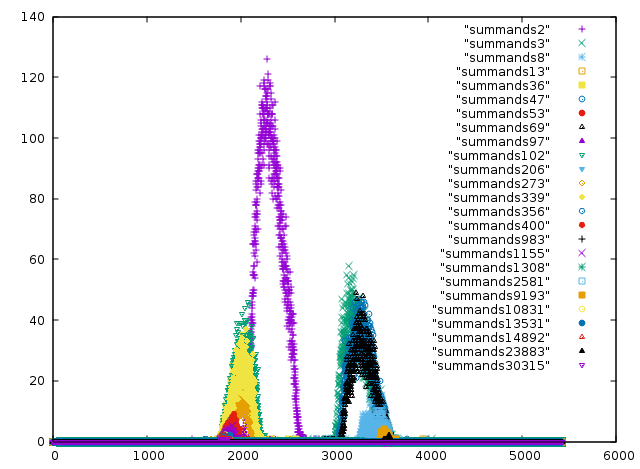
\includegraphics[scale=0.5]{../figs/summands_mod_5422.png}
\end{figure}

Since each of these seems to be instances of the same distribution
with different parameters, we might be interested in computing the
parameters of each, starting with the means.  This gives us table
\ref{tab:mean_comps}.

% for x in `ls`; do y=$(echo $x|sed 's/summands//'); z=$(echo '('$(cat $x|sed 's/\([0-9]\)[ \t]\+\([0-9]\)/\1*\2/' | tr '\n' '+' | sed 's/+$//;s/[ \t]//g')')/'$(cat $x|awk '{x
  % +=$2} END {print x}')|bc -l);  echo -e "$y\t$(((y*2219)%5422))\t$z"; done|sort -n -k 2

\begin{table}
\caption{Means of complements of $x \in \ulam{1}{2}$}\label{tab:mean_comps}
\centering
\begin{tabular}{lll}
  $a$     &$2219 a \mod {5422}$ & Mean of $2219 S_a \mod{5422}$ \\
  3	&1235	&3241.078\\
  47	&1275	&3288.007\\
  69	&1295	&3300.945\\
  8	&1486	&3431.555\\
  2581	&1607	&3485.878\\
  983	&1633	&3503.280\\
  206	&1666	&3518.475\\
  1308	&1682	&3525.956\\
  9193	&1703	&3541.352\\
  13	&1737	&3551.591\\
  23883	&1749	&3572.533\\
  30315	&3653	&1818.700\\
  13531	&3675	&1827.600\\
  14892	&3680	&1833.363\\
  10831	&3685	&1845.629\\
  53	&3745	&1872.413\\
  1155	&3761	&1883.377\\
  356	&3774	&1878.850\\
  97	&3785	&1891.297\\
  400	&3814	&1912.785\\
  273	&3945	&1984.791\\
  36	&3976	&1995.708\\
  339	&4005	&2013.333\\
  102	&4036	&2027.299\\
  2	&4438	&2319.242
\end{tabular}
\end{table}

Staring at that table for a minute, we notice that if we subtract the
second column from the third, we seen to get roughly 2000 for the
first 11 entries (those on the right end of the distribution).
Likewise, those on the left end (rows 12-25) seem to have a similar
pattern.

One possible reason for this is that the distribution we're taking the
mean of in the first row, say, is of $2219 a_n \mod{5422}$ where 3 is
a summand of $a_n$ in the Ulam sequence.  Since 3 is a summand of
$a_n$ in the sequence, we might instead look at the other summand of
$a_n$, i.e. $a_n - 3$.  This would lead to us not plotting
$2219a_n \mod {5422}$, but rather $2219(a_n-3) \mod{5422}$.  We can
compute these quickly and if we plot these, we get the plot in figure
\ref{fig:complements}.  That is, for each small summand $a$, we are
plotting a histogram for the set of ``complements'' of $a$: 
\[C_a = \{b \in A : a + b \in A\}\]

\begin{figure}
\caption{Distribution of $S_a - a$}\label{fig:complements}
\centering
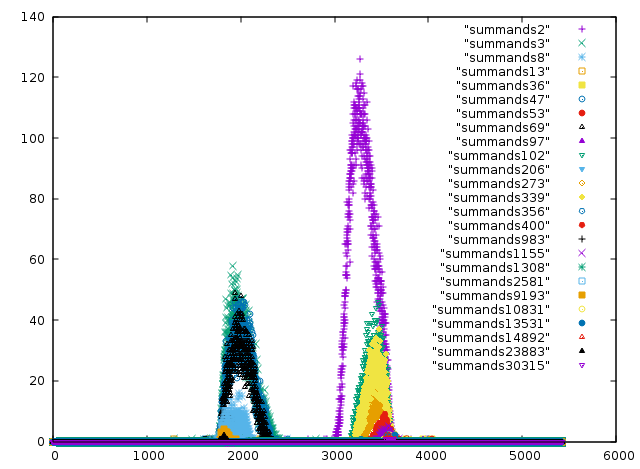
\includegraphics[scale=0.5]{../figs/shifted_summands_mod_5422.png}
\end{figure}

\section{Density}

One simple element of structure that we might hope to deduce from all
of this is some kind of positive density result for sum-free and Ulam
sequences.  For example, we note that for some large proportion of all
Ulam numbers $x$, then next Ulam number will be $x+2$.  For another
slightly smaller proportion, the next will be $x+3$.  So one approach
to studying the density would be to understand the structure of the
Ulam numbers well enough to be able to bound how often any given $d$
appears as a difference of consecutive Ulam numbers.

In this document we do not resolve this question either, but do give
conjectures in this direction.  However, one may note that the only
reason we know other Ulam sequences such as $\ulam{2}{5}$ have
positive density is that we know they are regular.  So in trying to
get a handle on the distribution of, say, $\ulam{1}{2}$, we expect
that any actual positive density result will come from an
understanding of its distribution, rather than vice-versa.

The first question is to attempt to compute the density of the various
sum-free sets and Ulam sequences that we are studying.  

\subsection{Computations}

The prescribed method for computing sum-free sets from a decision
sequence is already decently fast, provided we keep track of the data
appropriately.  Recall, the approach is to track three sets: $A$, the
actual sum-free set we are constructing, $D$, the set $A+A$ of things
that are ``disqualified'' from appearing in $A$, and $E$, the set of
things that are not disqualified by virtue of being sums but that,
according to the decision sequence, we are nevertheless to exclude.

We thus store $A$ as a list and $D$ as a hashset, (and need not keep
track of $E$).  So the algorithm is to, for each $x$ starting from 1
until we get bored:

\begin{enumerate}
\item Check if $x \in D$ (very fast, as $D$ is a hashset).  
\item If not, pop an item off the decision sequence.  
\item If 1, append $x$ in $A$ and add $x + A$ to $D$ ($|A|$ steps).
\end{enumerate}

So this algorithm to compute the first $N$ items will take
$O(N \cdot |A_N|)$ steps.

A similar algorithm can be implemented for the Ulam sequence, in fact:
Now, we track the set $A$ as a list, the hashset $D$ of disqualified
items (i.e. $x$ for which $r^*_{A+A}(x) > 1$), the sorted list $C$ of
candidates (i.e. $x$ bigger than every element of $A$ with
$r^*_{A+A}(x) = 1$), and a hashset $C'$ that also contains the candidates.  Then the algorithm is to initialise the
following: 

\begin{enumerate}
\item $A = [a,b]$
\item $C = [a+b]$
\item $C' = \{a+b\}$
\end{enumerate}

And proceed thus: 

\begin{enumerate}
\item Delete any inital elements of $C$ that are smaller than the
  largest element of $A$.  As we go, delete these elements from $C'$
  also.
\item Let $x$ be the first element of $C$, and append $x$ to $A$.
\item For each $a \in A$: Compute $x + a$ and, if it is in $C'$,
  delete it from $C'$ (fast, since $C'$ is a hashset) and from $C$
  (where we can find it by bisection, since $C$ is sorted).
\end{enumerate}

There is a more advanced algorithm that leverages the apparent bias of
such sequences as well, implemented in \cite{knuth:note}.  This speeds
the basic algorithm up by, among other things, noting that if we track
which elements of $A$ are outside the middle third mod $\lambda$ for a
$\lambda$ where there are few such elements, then when we're testing
whether any new $x$ within the middle third is actually a sum of
smaller elements of $A$, we only have to look at whether $x - a$ is in
$A$ where $a$ is one of the (hopefully few) elements of $A$ outside
the middle third.

In any case, the results of our computations give the estimates for
the densities of these sets found in label \ref{tab:densities}.

\begin{table}[ht]
\caption{Densities}
\label{tab:densities}
\centering
\doublespacing
\begin{tabular}{lll}
  $A$ & $|A_N|$ & $\delta_N$
  \csvreader{datafiles/density.csv}{}
  {\\$\csvcoli$ & \csvcolii & $\csvcoliii = \frac{1}{\csvcoliv}$}
\end{tabular}
\end{table}

\subsection{Constructions}

Another line of thought is to note that that the Ulam numbers are, in
some sense, as greedy as possible in their definition.  And while, for
example, $\theta(01001)$ is not maximally greedy, it is still greedy
$\frac25$ of the time.  So in the family of Ulam-like sets or sum-free
sets, if we have many positive-density examples, it seems unlikely
(though not impossible, as we shall see) that these very greedy sets
fail to be as high a density as possible.

We first start by noting that positive-density sum-free sets are
abundant, as a result of the abundance of sum-free sets
$A \subseteq \R/\Z$, coupled with the fact that if
$\pi_\lambda : \Z^+ \to \R/\Z$ by
$x \mapsto \frac{x}{\lambda} \mod{1}$, the inverse image
$\pi_\lambda\inv(A)$ is sum-free in the integers.  For example, the
set $A = \{1/2\}$ is sum-free in $\R/\Z$, and $\pi\inv_2(A)$ is the odd
positive integers, which is sum-free.  Likewise, the $A_\lambda$ from
earlier (for any irrational $\lambda$), where recall $A_\lambda$ was
the set of integers that, when reduced (in $\R$) modulo $\lambda$,
land in the interval $(\frac{\lambda}{3}, \frac{2\lambda}{3})$, are
also of this form.  So this kind of example gives many sum-free sets,
both regular and irregular, that all have positive density.

One might wonder whether we can similarly generate examples of
Ulam-like sets of positive density.  It turns out that one can do this
using the basic idea behind the $A_\lambda$ construction, but being
more careful about it.  But first, we will make precise what we mean
by ``Ulam-like'': 

Recall an Ulam sequence is an increasing sequence of positive integers
that starts with some $a$ and $b$ and that continues by choosing
integers according to the requirements of 1-additivity (``every
element is uniquely a sum of previous elements'') and greediness
(``always choose the smallest such element available'').  In some
ways, it is the greediness that makes Ulam sequences hard to analyse.
If we drop this condition, then we get a general class of sequences
which contains the Ulam sequences, but also many others:

\begin{definition}\label{def:1additive}
  For $S \subseteq \Z^+$ a finite set (say of size $k$), a
  \textbf{1-additive sequence with base $S$} is an infinite sequence
  of positive integers $a_i$ such that $a_1 < \ldots < a_k$ are the
  elements of $S$, and, for $n > k$, $a_n$ is greater than $a_{n-1}$
  and has a unique pair of integers $i, j$ with $0 < i < j < n$ such
  that $a_n = a_i + a_j$.

  We may talk of simply a \textbf{1-additive sequence}, by which we
  will mean a sequence of integers that is a 1-additive sequence with
  base $S$ for some $S$.
\end{definition}

\begin{example}
  \begin{enumerate}
  \item Any Ulam sequence $U(a,b)$ is 1-additive with base $a, b$.  
  \item The Fibonacci numbers $1, 2, 3, 5, 8, \ldots$ are a 1-additive
    sequence with base $1, 2$.  
  \item The set $\{2, 3, 5, 7, 9, \ldots\} = 2, 2+3\Z^+$ is 1-additive
    with base $2, 3$.  
  \item More generally, for any $a < b$, the set $a, b, b+a, b+2a,
    \ldots$ is 1-additive provided $b \neq 0 \mod{a}$.  
  \end{enumerate}
\end{example}

The last example gives plenty of examples of regular 1-additive
sequences.  (Indeed, $a = 2, b = 3$ provides an example of a set with
density apparently higher than that of $\ulam{2}{3}$ despite being
less greedy: It goes $2, 3, 5, 7, 9, 11, \ldots$, whereas a greedy
algorithm would include 8 as well.  Nevertheless, $\ulam{2}{3}$
appears to have density around $\frac{1}{10}$, whereas this less
greedy set has density $\frac{1}{2}$.)  

Nevertheless, all these examples are regular in the conventional
``mod-$m$'' sense.  So we might wonder what the analogue of
$A_\lambda$ for {\em irrational} $\lambda$ would be for 1-additive
sets.  Or, more simply, we might first ask whether there even is such
a thing as an irregular 1-additive set of positive density.  It turns
out that there is:

\begin{proposition}\label{prop:irr_1add}
  There exists an irregular 1-additive set of positive density.
\end{proposition}

The basic idea will be the following ``ping-pong mod $\lambda$''
construction: Take an irrational $\lambda$.  Take $a$ (the ``left
bat'') just above $0$ mod $\lambda$, and $b$ (the ``right bat'') just
below 0 mod $\lambda$, and a $c$ (the ``ball'') just above $\lambda/3$
mod $\lambda$.  The game will be to keep the ball in the set
$T = (\frac{\lambda}{3}, \frac{2\lambda}{3})$ (the ``table'') mod
$\lambda$ by adding $a$ to it until it reaches the right side, then
adding $b$ to it until it reaches the left side, and repeating
indefinitely.

Supposing we are a little careful about our choices of $a, b, c$, and
$\lambda$, we should be able to show that this construction satisfies
the required properties.

\begin{proof}
  More precisely: start with an irrational $\lambda$, an $a$ with
  $a \mod{\lambda}$ lying in $(0, \frac{\lambda}{12})$, and a $b > a$
  with $b \mod{\lambda}$ in $(\frac{11\lambda}{12},\lambda)$, and a
  $c > b$ with $c \mod{\lambda}$ in
  $(\frac\lambda 3, \frac\lambda 2)$, and say further that $a \nmid b$
  (for reasons that will become apparent later).  Also, let
  $T = (\frac{\lambda}{3}, \frac{2\lambda}{3})$.

  Then we will define a sequence of sets $A_n$ which will comprise the
  sequence $A$, as follows: Let $c_1 = c$.  For $n \geq 1$, let
  $A_n = \{c_n + ka : k \in \Z^+, c+ka\mod{\lambda} \in T\}$ if $n$ is
  odd, and $A_n = \{c_n + kb : k \in \Z^+, c+ka\mod{\lambda} \in T\}$
  if $n$ even.  Let $c_{n+1}$ be the largest element of $A_n$
  (allowing the definition of $A_{n+1}$ to make sense).

  Then let $S = \{a, b, c\}$ and $A = S \cup \bigcup_{i=1}^\infty
  A_i$.  

  Now let us check the definition: Our base set is $S$.  Every element
  $a_i$ has $a_i < a_{i-1} + a + b$, so the set is has positive
  density.  $A$ is not dense mod $\lambda$ (since all but three
  elements are in $T$) whereas any regular set would have to be (since
  $\lambda$ is irrational), so $A$ cannot be regular.  It remains to
  check 1-additivity.

  By construction, every element $a_n > c$ is either $a_{n-1} + a$ or
  $a_{n-1}+b$, so every element not in $S$ is a sum of smaller
  elements in at least one way.  Now suppose $a_n$ is a sum of smaller
  elements in another way also.  Then because $a_n$ is in $T$, it
  cannot be a sum of two other elements in the middle third.  Thus the
  only for $a_n$ to be a sum of other elements of $A$ in two different
  ways is if $a_n - a$ and $a_n - b$ are both in $A$.

  But now, say $a_n = c + ax + by$, for some $x \geq 0, y \geq 0$.  We
  know that $a_n \in A_i$ for some $i$.  If $i$ is even, then by
  definition, the previous element of $A$ will be $a_n - b$, and
  $a_n - b < a_n - a < a_n$, so $a_n - a$ cannot be in $A$.

  If instead $i$ is odd, then $a_n - a \in A$.  Then say
  $a_{n-r} = \max A_{i-1}$, so $a_n = a_{n-r} + ra$ (and we know
  $r \geq 1$, since $a \in A_i$ for odd $i$).  Thus
  $a_{n-r} = c + a(x-r) + by$.  Then the element before this in $A$
  would be $c + a(x-r) + b(y-1) < a_n - b$.  Thus for $a_n - b$ to be
  in $A$, it would have to be an element after $c + a(x-r) + b(y-1)$.
  But all these elements are got by adding $a$ to $a_{n-r}$.  So
  $a_n - b$ has the form $c + a(x-s) + by$ for $0 \leq s \leq r$.  But
  $c + a(x-s) + by = c + ax + by - b$ implies $as = b$, which
  contradicts $a \nmid b$, which was our condition on $a$ and $b$.

  Thus $a_n - a$ and $a_n - b$ can never both be in $A$, making $A$
  also 1-additive.
\end{proof}

We note, however, that this construction gives us a 1-additive set
with a base of size 3, whereas the Ulam numbers are a 1-additive set
with a base of size 2.  So we might wonder whether there is a similar
(if more complicated) construction of this sort.

The following construction, we believe should work: 

\begin{conjecture}
  There is an irregular, positive density 1-additive set with a base
  of size 2.
\end{conjecture}

To try this, we will play the same game of ping-pong, but now we are
only allowed to use two elements.  We will again start with an
irrational $\lambda$ and $a \in \Z^+$ the ``left bat'' in the range
$(\frac{\lambda}{6}, \frac{\lambda}{3})$ mod $\lambda$.  But now we
will start with $c$ being the ``ball'' inside the ``table''
$T = (\frac{\lambda}{3}, \frac{2\lambda}{3})$.

Then we will add $a$ to $c$ until it comes out on the right side as
some $b \in (\frac{2\lambda}{3}, \frac{5\lambda}{6})$, and that will
be our ``right bat''.  Then we will do roughly the same thing as
before, except now $a$ and $b$ have larger magnitude mod $\lambda$, so
they may occasionally hit the ball off the table slightly.  This will
give us further bats with which to hit the ball--usually bats with
even greater magnitude mod $\lambda$.  The idea, then, will be to
always hit the ball with the smallest available bat (in the sense of
$\normrz{x}$) that doesn't send it off the table (when possible), so
that there is the most flexibility for the other side to ensure they
are also able to hit the ball back onto the table.

If we plot the first 100 elements of $\ulam{1}{9}$ by plotting $n$ on
the $x$-axis, and $a_n \mod{\lambda}$ on the $y$-axis, then we get a
picture that shows something of this kind happening in figure
\ref{fig:pingpong}.  In this picture, the horizontal lines are placed
at $\frac{k\lambda}{6}$ for $k = 0, \ldots, 6$.  So we see that $1$ is
very close to the left side mod $\lambda$, and so functions as the
``left bat'', while every time we go off the other side of the table,
we get a new ``right bat'', which we can use to move things back to
the left when they get too close to the edge.

\begin{figure}
\caption{$(n, a_n \mod{\lambda})$ for $\ulam{1}{9}$ and $n \leq 100$}\label{fig:pingpong}
\centering
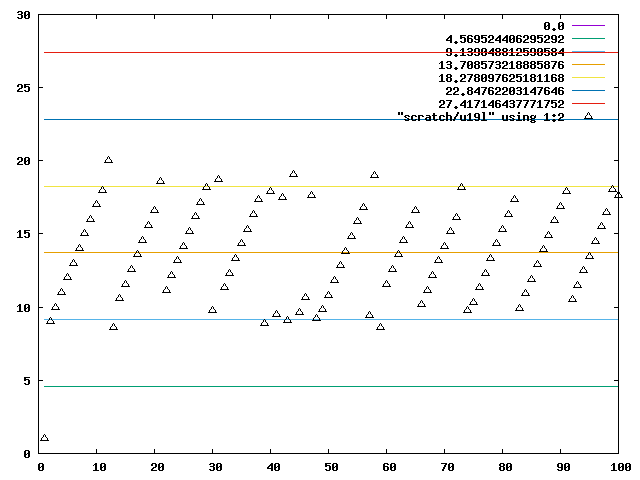
\includegraphics[scale=0.5]{../figs/u1_9_pingpong.png}
\end{figure}

\subsection{Conjectures}

Recall that sum-free sets of positive integers correspond bijectively
with binary ``decision'' sequences.  We know also that there are many
sum-free sets of positive density.  Further, we can easily see that if
the 1s have zero density in the decision sequence, then the resulting
sum-free set has zero density.  So all the positive-density sum-free
sets must have decision sequences with positive density.  

\begin{question}
  For any decision sequence $S$ with a positive density of 1s, the
  corresponding sum-free set $A = \theta(S)$ has positive upper density.
\end{question}

\begin{conjecture}
  For any decision sequence $S$ that is eventually periodic and for
  which the repeating pattern has at least one 1, then the
  corresponding sum-free set $A = \theta(S)$ has positive upper
  density.
\end{conjecture}

As we have said, it appears that the Ulam sequence has positive
(upper) density around $0.07$.  This, together with the ultimate
greediness of the Ulam sequence suggests for us the conjecture:

\begin{conjecture}
  The Ulam sequence $\ulam{1}{2}$ has positive upper density.
\end{conjecture}

\chapter{Future Directions}

In this section, we outline some possible future avenues of study,
both for extending our main line of thought here as well as for
answering separate, related questions.  

\section{Technology}

There are a number of results and techniques that have seen
application to related problems that we suspect may allow for further
progress in future study of this problem.  

\subsection{Triangle removal}

Throughout much of this study, we have been treating sum-free sets and
other \relevant sets more or less simultaneously.  However, in many
ways sum-free sets are less rigid and are easier to reason about,
whether via the correspondence with decision sequences or in the ease
of constructing examples with certain desired features.

We have also noted that the Ulam sequence has few small summands.  In
particular, if $S$ is the set of small summands, then we can partition
the Ulam numbers $A$ into $S \cup T$ where $T$ is sum-free, and $S$
seems to be small.  A result about the size of $S$ could allow us to
reduce general questions about 1-additive and other \relevant sets to
questions just about sum-free sets.  One general result in this
direction comes from Green \cite{green:gfa2005} (Cor. 1.6) in the
following theorem:

\begin{theorem}\label{thm:green_triangle_removal}
  There is a universal function $f(\delta)$ with $f(\delta) \to 0$ as
  $\delta \to 0$ such that the following holds: For any $N > 0$ and
  any subset $A \subseteq [N]$ with $\delta N^2$ solutions to $x+y=z$.
  Then there is a partition of $A$ as $A = B \cup C$ where $B$ and $C$
  are disjoint, $B$ is sum-free, $C$ is small: $|C| \leq f(\delta)N$.
\end{theorem}

In the case of the Ulam numbers, assuming they have positive density
$\delta$, then $A_N$ hae at most $3\delta N$ solutions to $x+y=z$.
That is, $A_N$ has $\frac{3\delta}{N} N^2$ solutions, meaning this
theorem gives us a $A_N = B_N \cup C_N$ where
$|C_N| \leq f(\frac{3\delta}{N})N$ and $B_N$ is sum-free.  However,
this notation is slightly misleading: There isn't a guarantee that
there is one whole set $C \subseteq \N$ such that $C_N = C \cap [N]$
as $N$ grows.  It also does not guarantee that $C$ is in any way
related to $S$, and so does not gives us a numerical bound on $|S_N|$
as $N$ grows.  Thus we have a question:

\begin{question}
  Can we estimate $|S_N|$ associated to a 1-additive set $A$?  Say,
  can we prove $|S_N| = \Theta(\log(N))$?  (For example, if we plot
  the logarithm of the $i$th small summand against $i$, we get figure
  \ref{fig:log_ss}.)  Specifically, perhaps, can we take the proof of
  theorem \ref{thm:green_triangle_removal} and in the particular case
  of the Ulam numbers get a good bound for $f$?
\end{question}

\begin{figure}
\caption{$\log(s_i)$ for small summands $s_i$ plotted against
  $i$}\label{fig:log_ss}
\centering
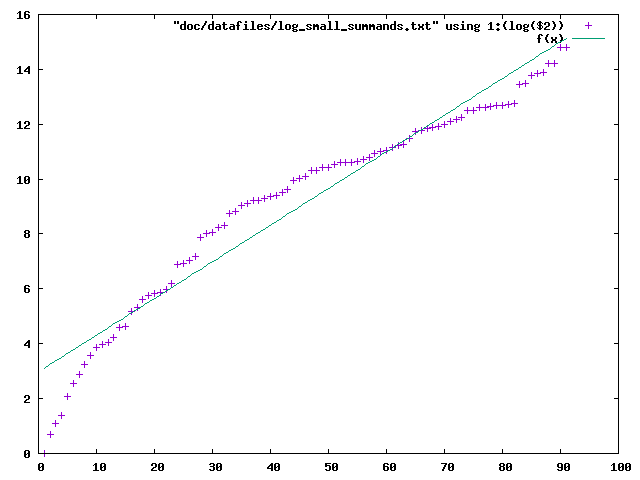
\includegraphics[scale=0.5]{../figs/log_ss.png}
\end{figure}

\subsection{Ultralimits}

The phenomenon we have been addressing appears to be one that remains
true in some kind of limit.  However, the precise statement of this
seems delicate.  For example, trying to prove that there is a non-zero
$\alpha\in\R/2\pi\Z$ with $\widehat{A}(\alpha) \neq 0$ in the sense of
definition \ref{def:fourier} is fraught with tricky convergence
issues.  In \cite{tao:ams2012}, Tao outlines an argument for Roth's
theorem using ultralimits that manages to work entirely in the
infinitary setting and deduce the finite structure (namely, 3-term
arithmetic progressions) that is desired.  It may be worth exploring
whether this technique applies in the Ulam case as well, whether to
simplify the arguments we have given or to prove more than we have
managed here.

\subsection{Energy increment}

Considering the mileage we got out of imitating the classic ``density
increment'' proof of Roth's theorem, we might turn to looking at other
methods of proof and seeing what those tell us about Ulam sequences
also.  One such relies on the so-called Szemeredi regularity theorem,
which is in turn proven by a technique that appears repeatedly in
additive combinatorics: The ``energy increment'' argument.  

Broadly, this type of argument (as described in \cite{tao:cup2006})
goes by quantifying the presence of a certain kind of structure in a
function by an ``energy''.  Then, we approximate our given function
with a low-complexity approximation function (for example, the
indicator function of a set can be approximated at first by the
constant function whose value is the density of the set).  The
argument then proceeds to use a dichotomy, much as in the density
increment case: If the energy of this approximation is large, then
there is a lot of the desired structure and we are done.  If the
energy is small, then this implies some bias (such as, in the case of
Roth's theorem, a large Fourier coefficient) that we can use to find a
better approximation with increased energy.  Executing this enough
times, we force our approximation into the large energy setting where
we can win.

So if we could pin down a more general notion of regularity (such as a
precise quantification of ``bias modulo some $\lambda$''), then we
might be able to follow a similar plan: Assign a notion of ``energy
modulo $\lambda$'' to the distribution that is large if the
distribution is very non-uniform, say.  Then, approximate the
indicator function $A$ of $\ulam{1}{2}$ on $[N]$ by
$\delta = \frac{|A_N|}{N}$.  If this has low energy, prove that the
difference between the function and our approximation has Fourier bias
(as in \ref{thm:alpha}) and therefore some correlation with a
non-uniform distribution (as in \ref{thm:regularity}), and use that to
better approximate the indicator function with something of higher
energy (i.e., more bias).

This plan would first require having a precise notion of ``energy''
that captures whatever notion of ``regularity'' we would ultimately
hope to prove for $\ulam{1}{2}$.

\subsection{Arithmetic regularity}

The ultimate consequence of many energy increment type arguments is a
very general sort of regularity theorem, from Szemeredi's regularity
theorem to the more arithmetically flavoured regularity results of
Green and Tao \cite{green:bsm2010}.  In that paper, the arithmetic
regularity theorem in particular was used to prove Roth's theorem
directly, and it has been used to study sum-free subsets of integers
to great effect in \cite{eberhard:ann2014}.  In particular,
\cite{eberhard:ann2014} works with sum-free sets using a kind of
``local-to-global'' argument that has a similar flavour (if very
different content) to what we are looking for.

A likely fruitful future direction, then, would be to understand the
implications of such regularity results for Ulam numbers.  

\section{Variants of the Ulam problem}

We have already described 1-additive sets (see definition
\ref{def:1additive}) in greater generality than just the Ulam numbers.
We could either modify the initial ``seed set'' or we could be less
greedy about picking the next elements, but fundamentally, these sets
are all \relevant and so we expect to be able to say the same things
about them.  There are, however, other modifications that may be worth
considering for the purpose of being able to prove things, which we
discuss in this section.

\subsection{Sums of more than two previous elements}

One modification is that our notion of 1-additive used only sums of
two elements.  We could equally define: 

\begin{definition}\label{def:1k_additive}
A $(1,k)$-additive set is a set $A \subseteq \N$ with an $N$ such
that, for $x > N$, there is exactly one way to write $x = a_1 + \ldots
+ a_k$ for $a_i \in A$ and $a_1 < \ldots < a_k$.  
\end{definition}

This we would expect to behave similarly, but one consideration draws
us to this type of set specifically: When we were trying before to
estimate $r_{A+A}(x)$ using the large spectrum $\alpha\Z$, this
essentially amounted to using the circle method.  In classical
applications of the circle method, (for example, the proof of
Vinogradov's theorem), we find that the circle method is much better
at counting representations of a given $x$ by sums of $k$ elements of
a set $A$ for larger $k$ than for, say, $k = 2$ (which in the
Vinogradov case would be the Goldbach conjecture).

This might lead us to suspect that $(1,k)$-additive sets may be even
more susceptible to circle method analysis for larger $k$ than
$k = 2$, which is the case we have been dealing with.

\subsection{Probabilistic versions}

One thing we get from the bijection between sum-free sets and infinite
binary sequences is a probability measure on all sum-free sets, taken
from the measure on binary sequences that considers each entry as a
flip of a fair coin (or, if desired, of a weighted coin).  This leads
to natural questions about the structure of random sum-free sets,
which have been studied in \cite{cameron:ptrf1987} and
\cite{calkin:dm1998}.

Considering Ulam numbers as an extension of the idea of sum-free sets
to considering sets $A$ whose elements $x$ have $r_{A+A}(x)$ small, we
might try to define a random version of this.  For example we can
construct a random 1-additive set: 

\begin{definition}
  Let $A$ be a set consisting of a finite ``seed set'' $S$, and then
  being built by the following random process: Given the current set
  of elements in $A$, let $A_1$ be the set of elements
  $x \in \N, x > \max(A)$ such that $r^*_{A+A}(x) = 1$.  Select an
  element uniformly at random from $A_1$ and include that element in
  $A$.  Repeat forever.  
\end{definition}

Or, we could define a random construction of a set that simply has
small values for $r_{A+A}(x)$ for $x \in A$: 

\begin{definition}
Let $A$ be a set consisting of a finite ``seed set'' $S$, and then
being built by a random process that takes each $x$, computes
$r_{A+A}(x)$ using the elements included in $A$ thus far, and includes
$x$ with probability $\frac{1}{r_{A+A}(x)}$ (including it
automatically if $r_{A+A}(x) = 0$, say.)
\end{definition}

Having such definitions in hand, we can then ask probabilistic
versions of all the questions we have asked about density, Fourier
spectrum, distribution, and structure that we have asked about the
Ulam numbers.

%%%%%%ENDDOC

\bibliography{doc}{}
\bibliographystyle{plain}

\end{document}